\newpage
\appendix
\section{Appendix}
\counterwithin{figure}{section}
\setcounter{figure}{0}
\counterwithin{table}{section}
\setcounter{table}{0}
\noappendixindent

\subsection*{A1. Phylogenetic Analysis}
\normalsize
All shown phylogenetic trees have been visualized with Dendroscope \cite{huson2012}.

\begin{figure}[h!tbp]
    \centering
    \renewcommand{\thefigure}{A\arabic{figure}}
    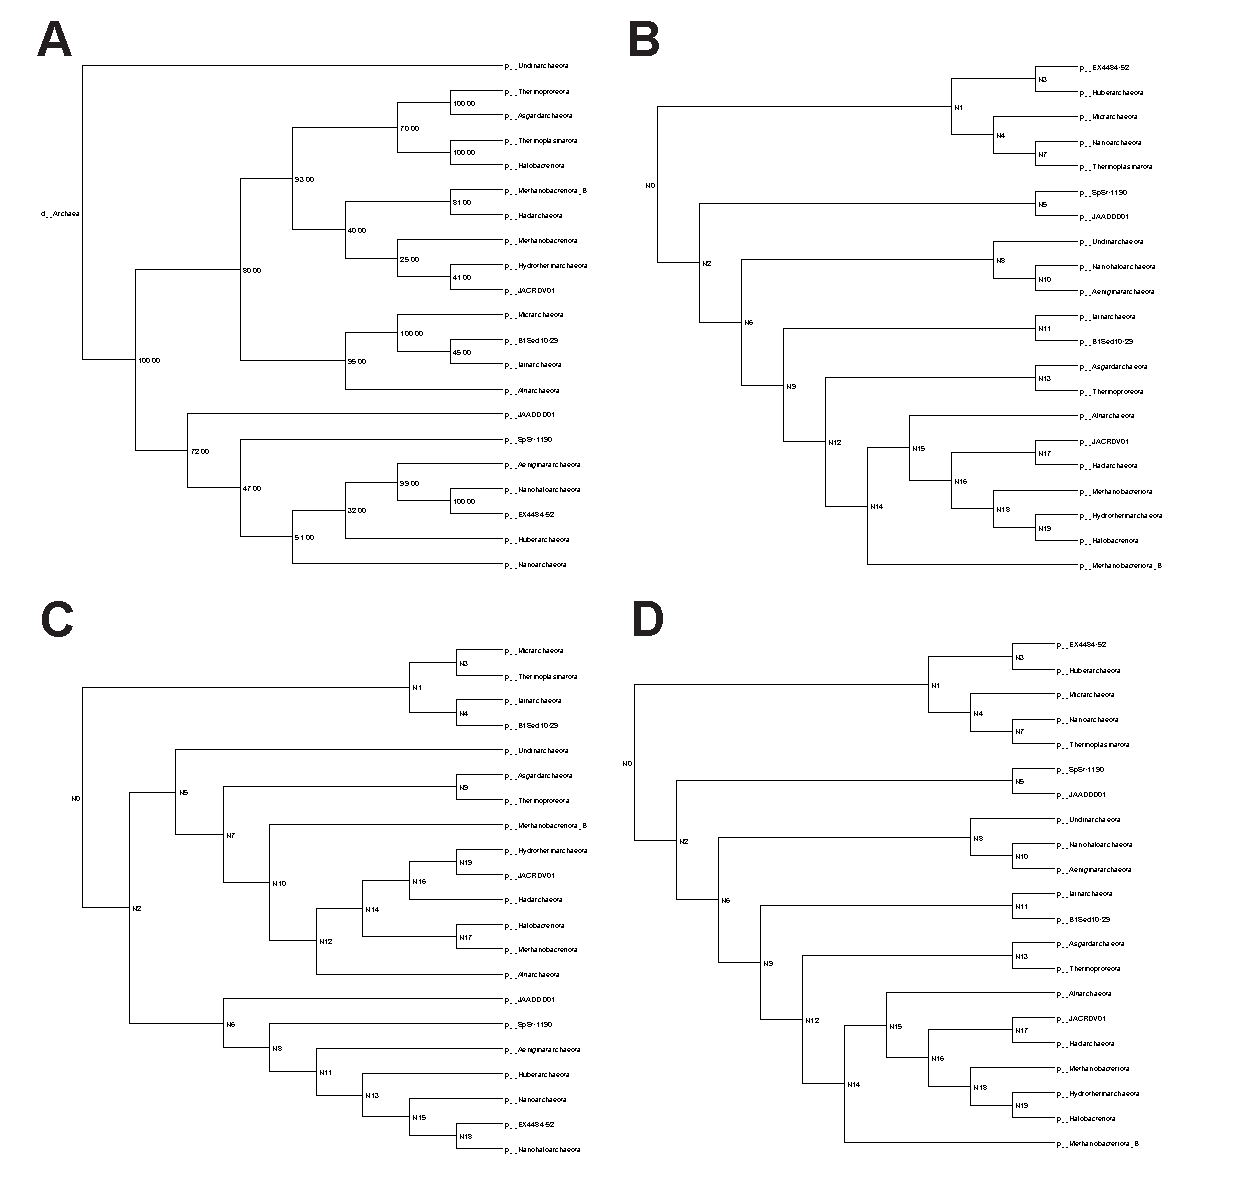
\includegraphics[width=0.95\textwidth]{trees/all_trees.pdf}
    \caption{Archaea species trees. (A) GTDB-inferred species tree. (B) OrthoFinder-inferred species tree; first analysis. (C) OrthoFinder-inferred species tree; second analysis. (D) OrthoFinder-inferred species tree; third analysis.}
    \label{phylum_trees_all}
\end{figure}


% \begin{figure}[h!tbp]
%     \centering
%     \renewcommand{\thefigure}{A\arabic{figure}}
%     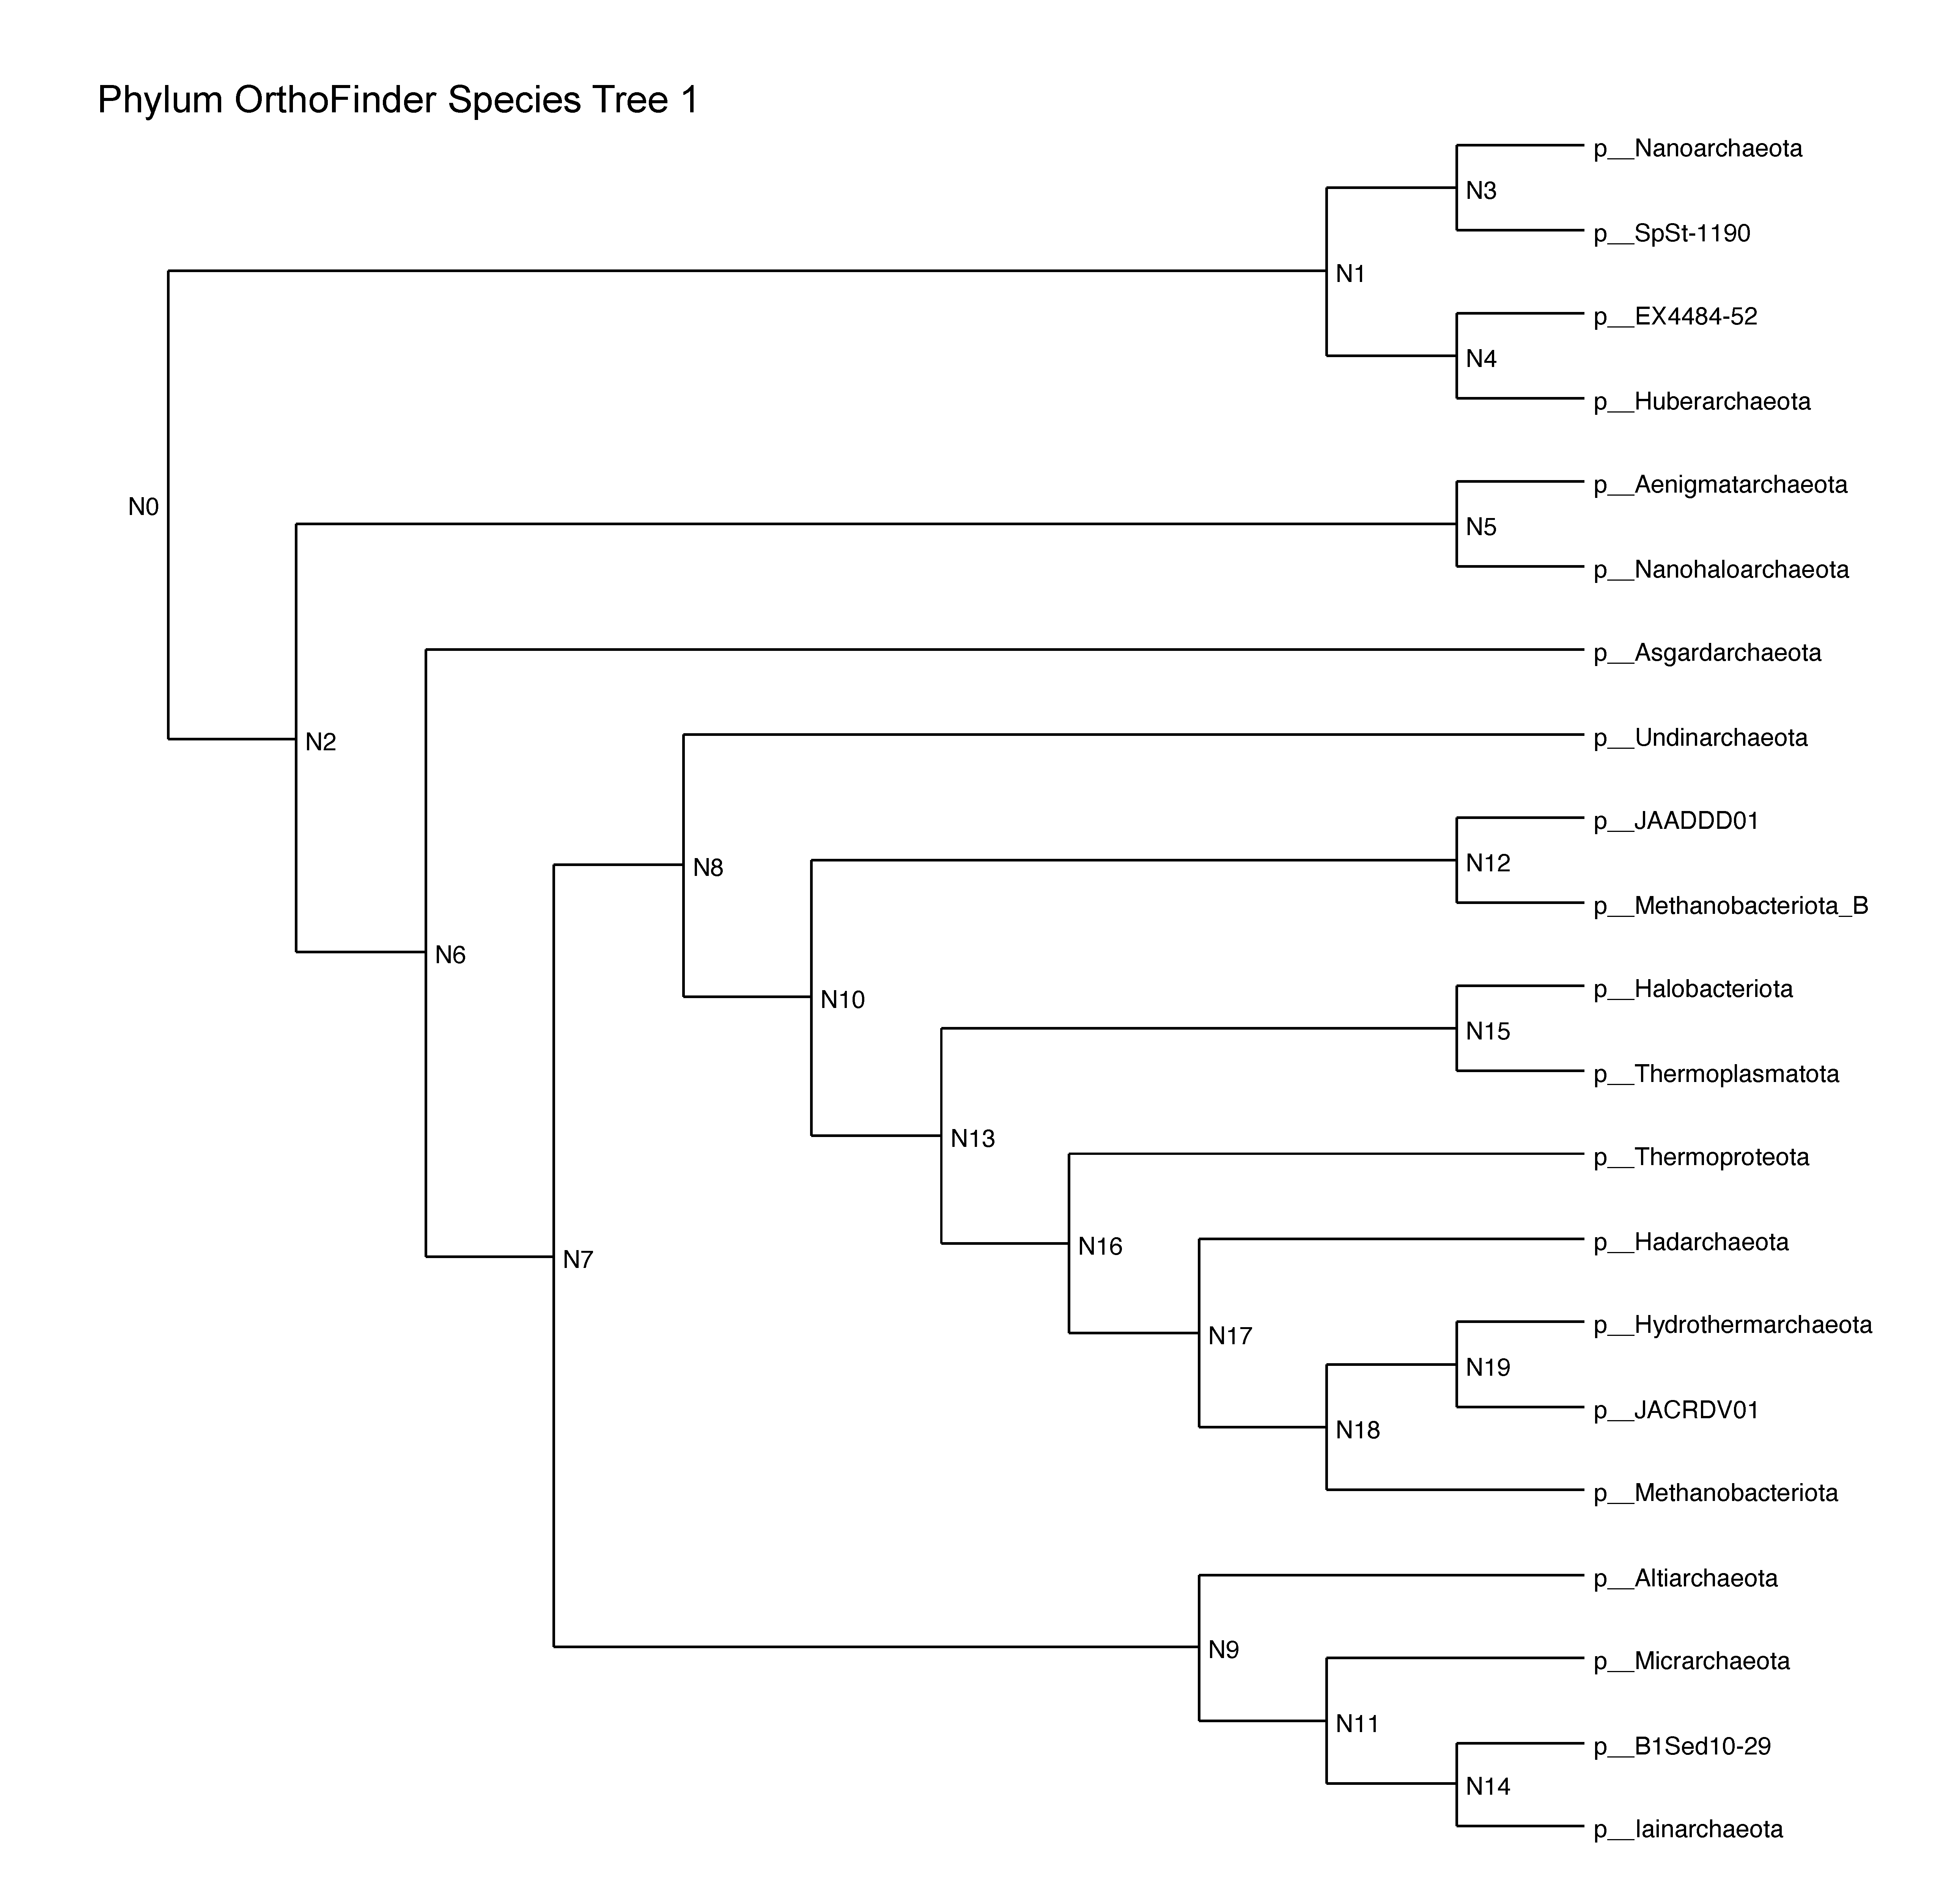
\includegraphics[width=0.5\textwidth]{trees/phy1arc}
%     \caption{OrthoFinder-inferred species tree; first analysis.}
%     \label{phylum_trees1}
% \end{figure}

% \begin{figure}[h!tbp]
%     \centering
%     \renewcommand{\thefigure}{A\arabic{figure}}
%     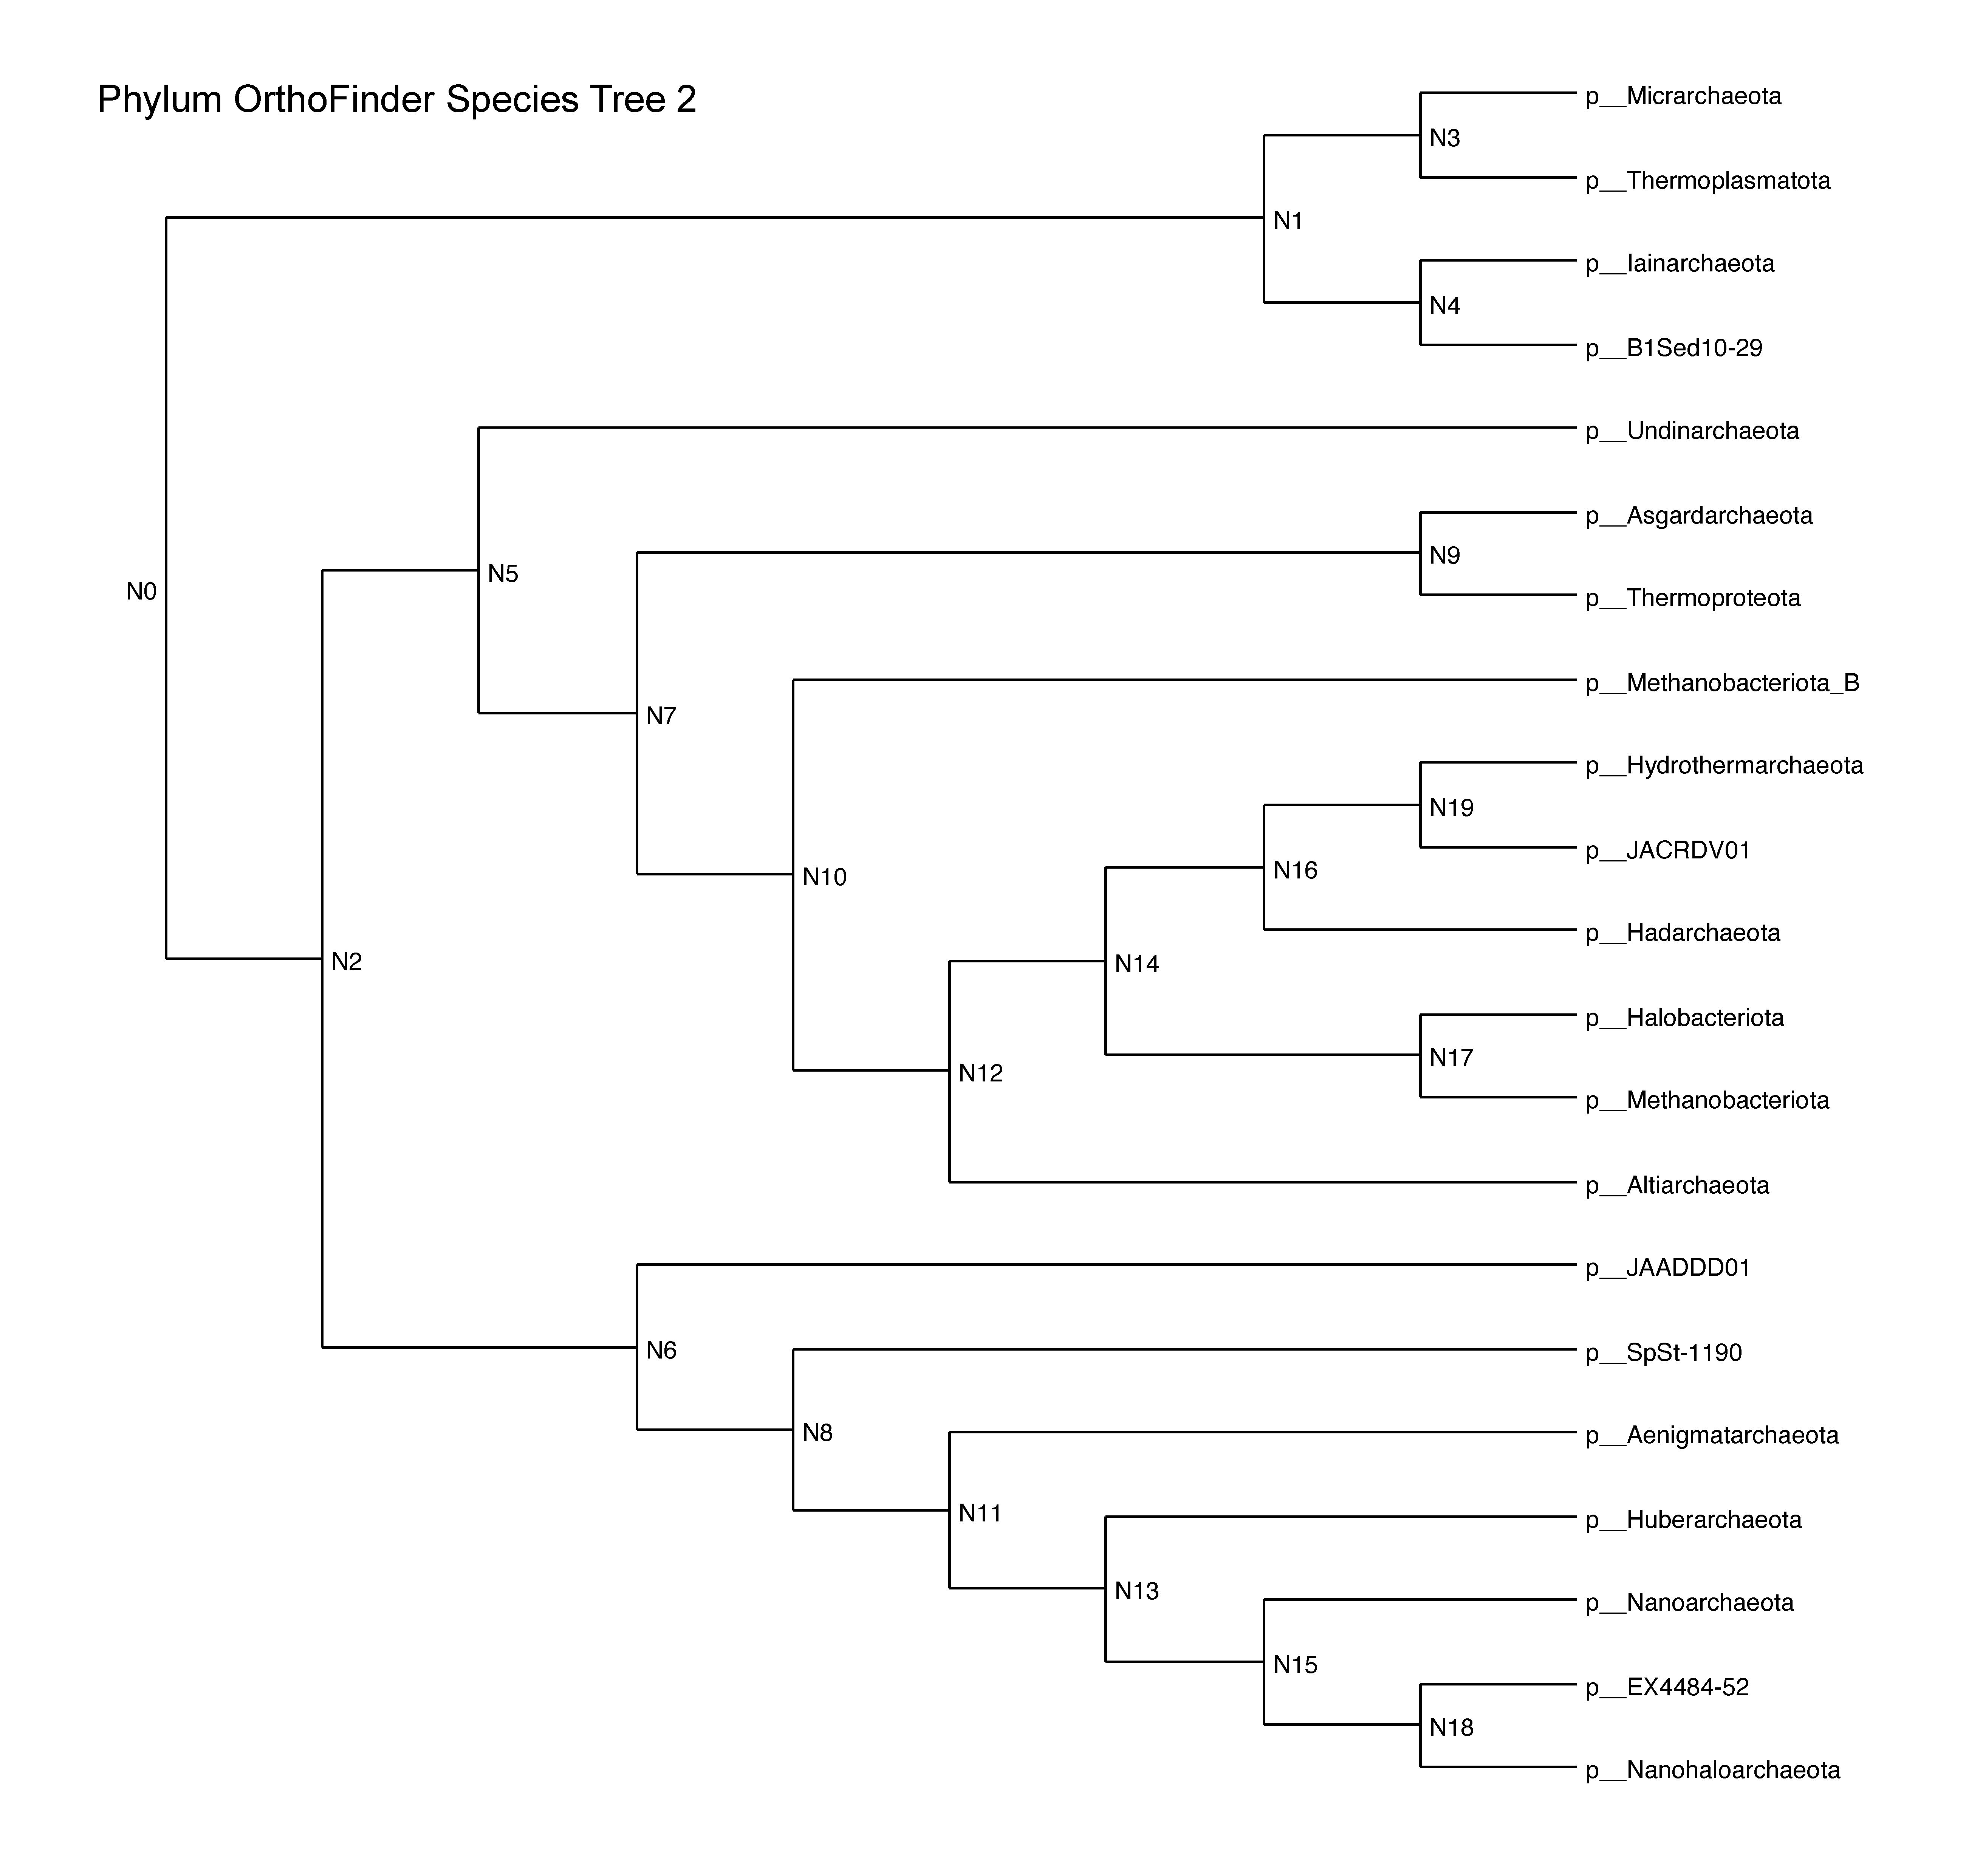
\includegraphics[width=0.5\textwidth]{trees/phy2arc}
%     \caption{OrthoFinder-inferred species tree; second analysis.}
%     \label{phylum_trees2}
% \end{figure}

% \begin{figure}[h!tbp]
%     \centering
%     \renewcommand{\thefigure}{A\arabic{figure}}
%     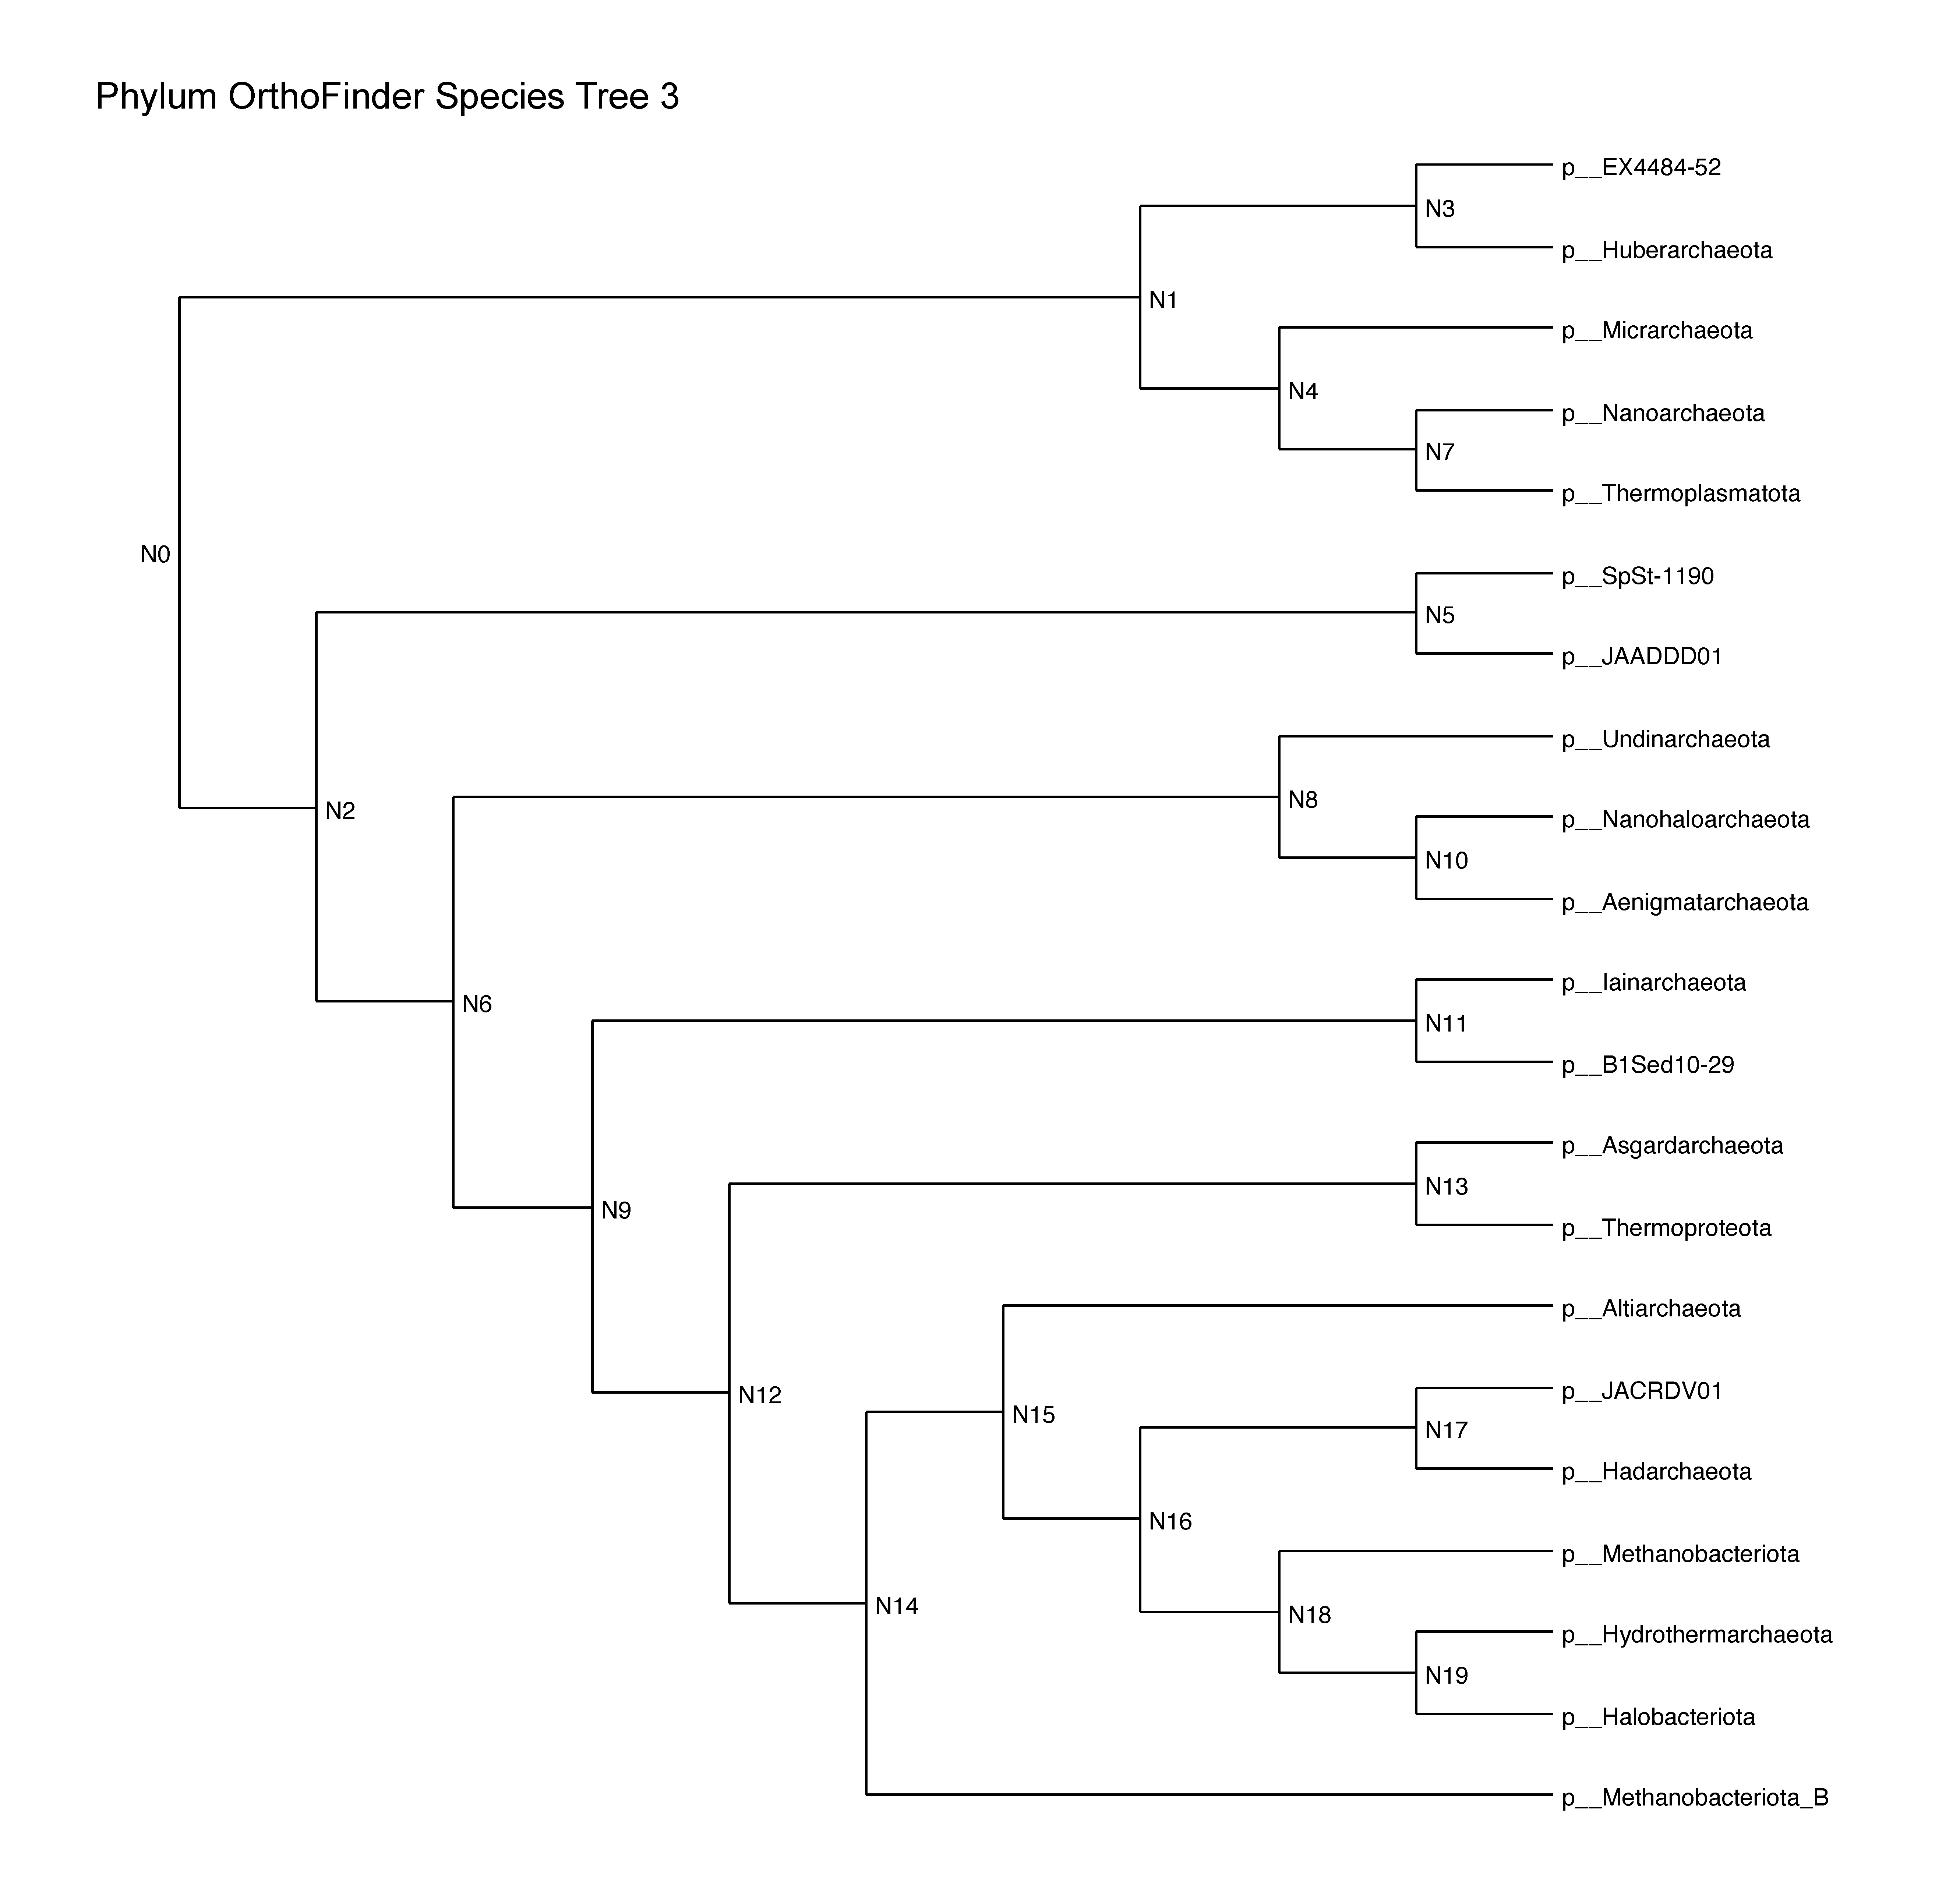
\includegraphics[width=0.6\textwidth]{trees/phy3arc}
%     \caption{OrthoFinder-inferred species tree; third analysis.}
%     \label{phylum_trees3}
% \end{figure}

% \begin{figure}[h!tbp]
%     \centering
%     \renewcommand{\thefigure}{A\arabic{figure}}
%     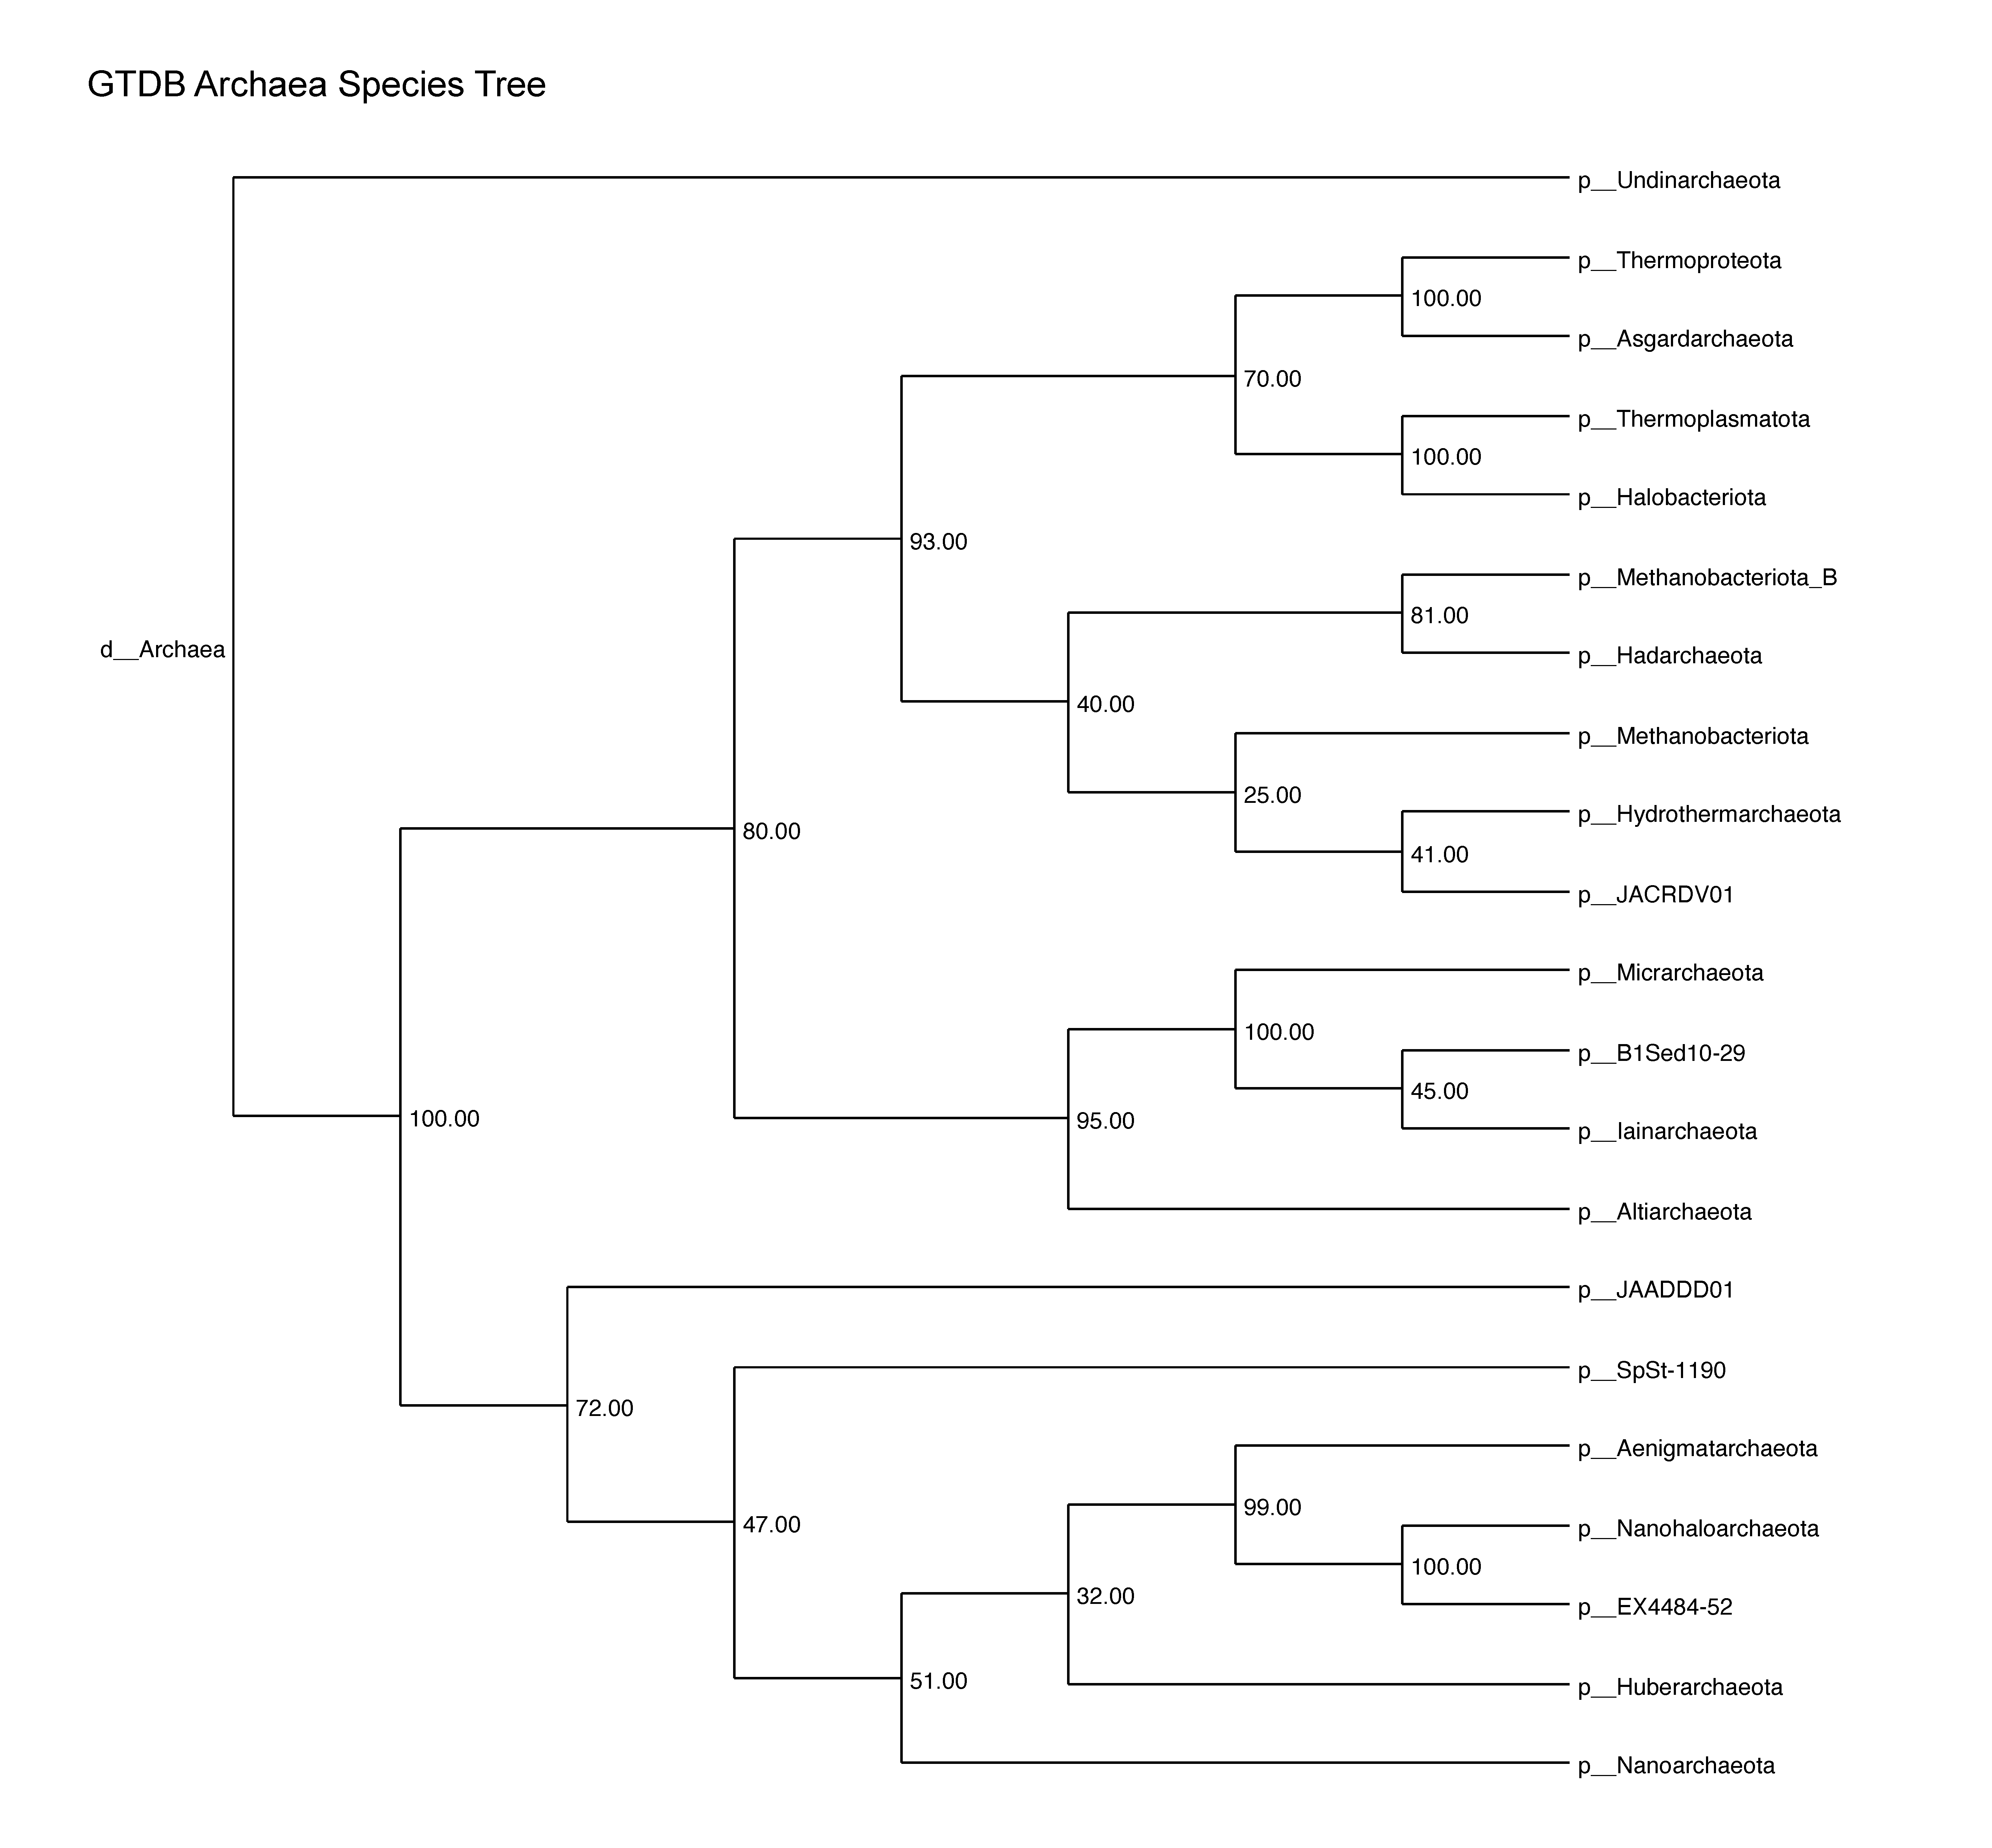
\includegraphics[width=0.6\textwidth]{trees/gtdb_tree}
%     \caption{GTDB archaea species tree.}
%     \label{gtdb_tree}
% \end{figure}

\newpage
\subsection*{A2. Metabolic Network Reconstruction of LACA for all Archaea Datasets}
\textbf{Metabolic Potential of LACA.}

\begin{figure}[H]
    \centering
    \includegraphics[width=0.95\textwidth]{metabolism/phy_arc_n0.pdf}
    \caption{Reconstruction of LACA's metabolic network from extant life, for the phylum-level archaea dataset. In black: enzymes and metabolic pathways that were inferred to be present in LACA.}
    \label{phy4arc_metnet}
\end{figure}   

\begin{figure}[H]
    \centering
    \includegraphics[width=0.95\textwidth]{metabolism/cla_arc_n0.pdf}
    \caption{Reconstruction of LACA's metabolic network from extant life, for the class-level archaea dataset. In black: enzymes and metabolic pathways that were inferred to be present in LACA.}
    \label{cla4arc_metnet}
\end{figure}   

\begin{figure}[H]
    \centering
    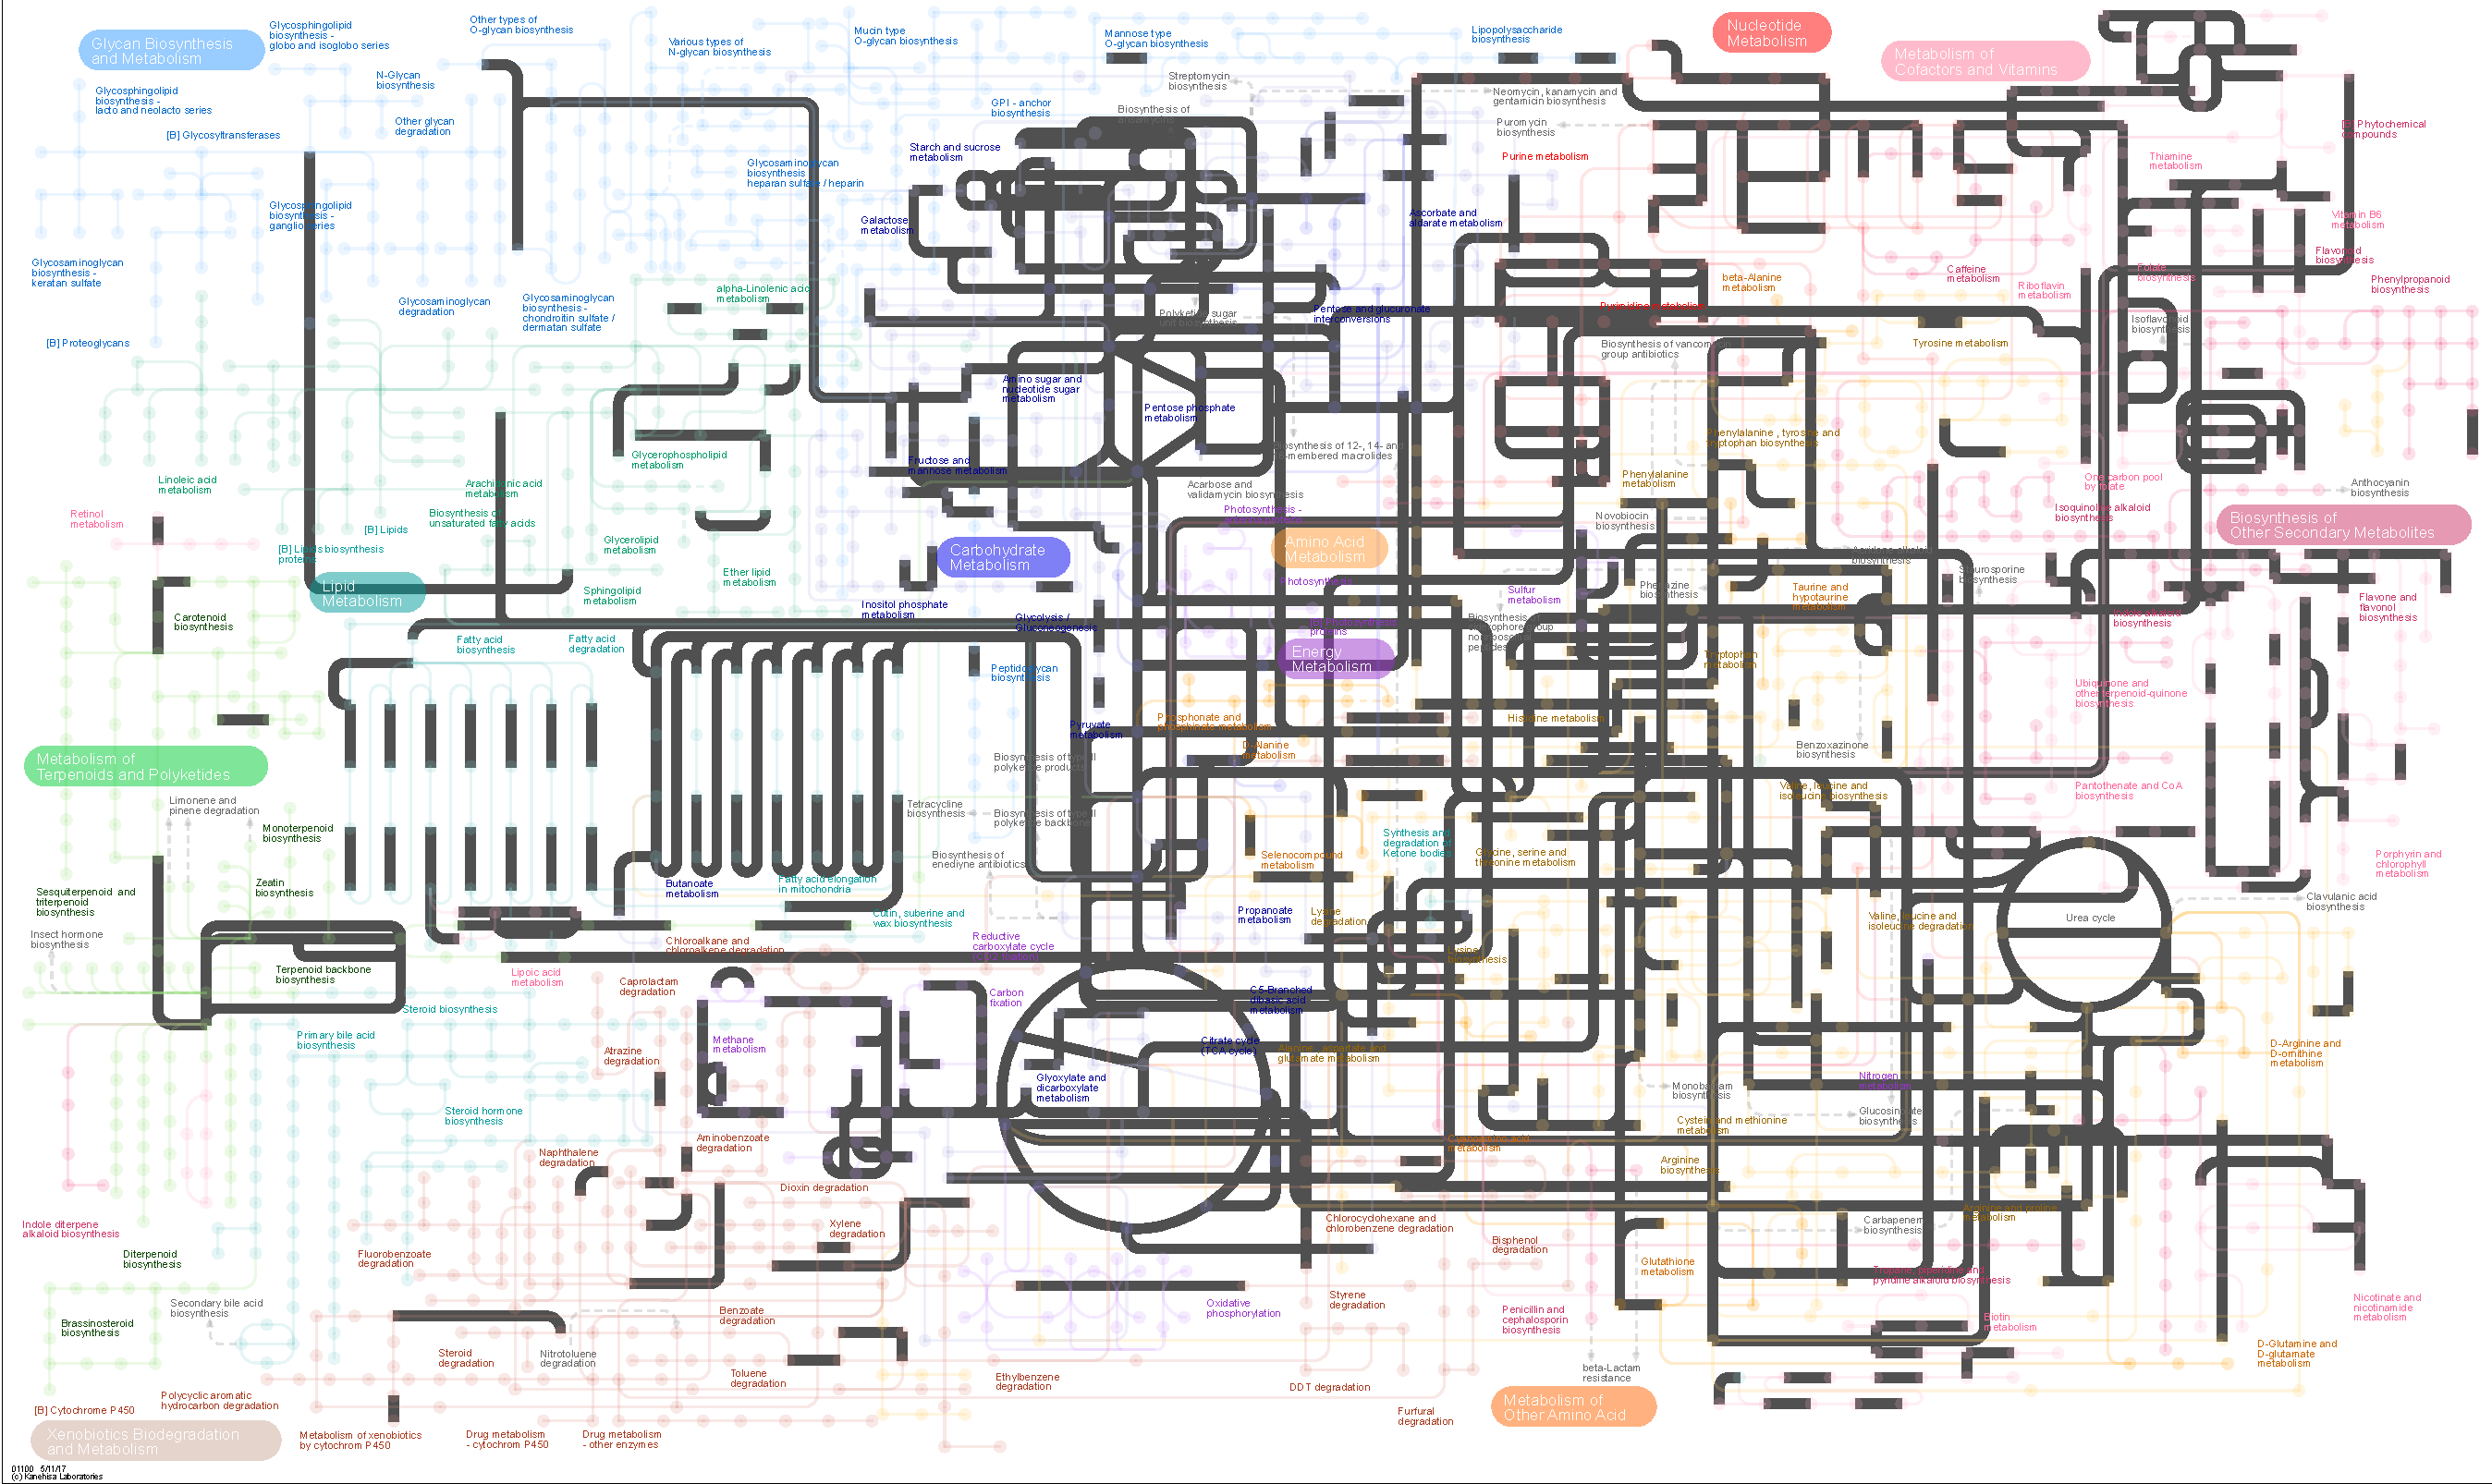
\includegraphics[width=0.95\textwidth]{metabolism/ord_arc_n0.pdf}
    \caption{Reconstruction of LACA's metabolic network from extant life, for the order-level archaea dataset. In black: enzymes and metabolic pathways that were inferred to be present in LACA.}
    \label{ord4arc_metnet}
\end{figure}   

\begin{figure}[H]
    \centering
    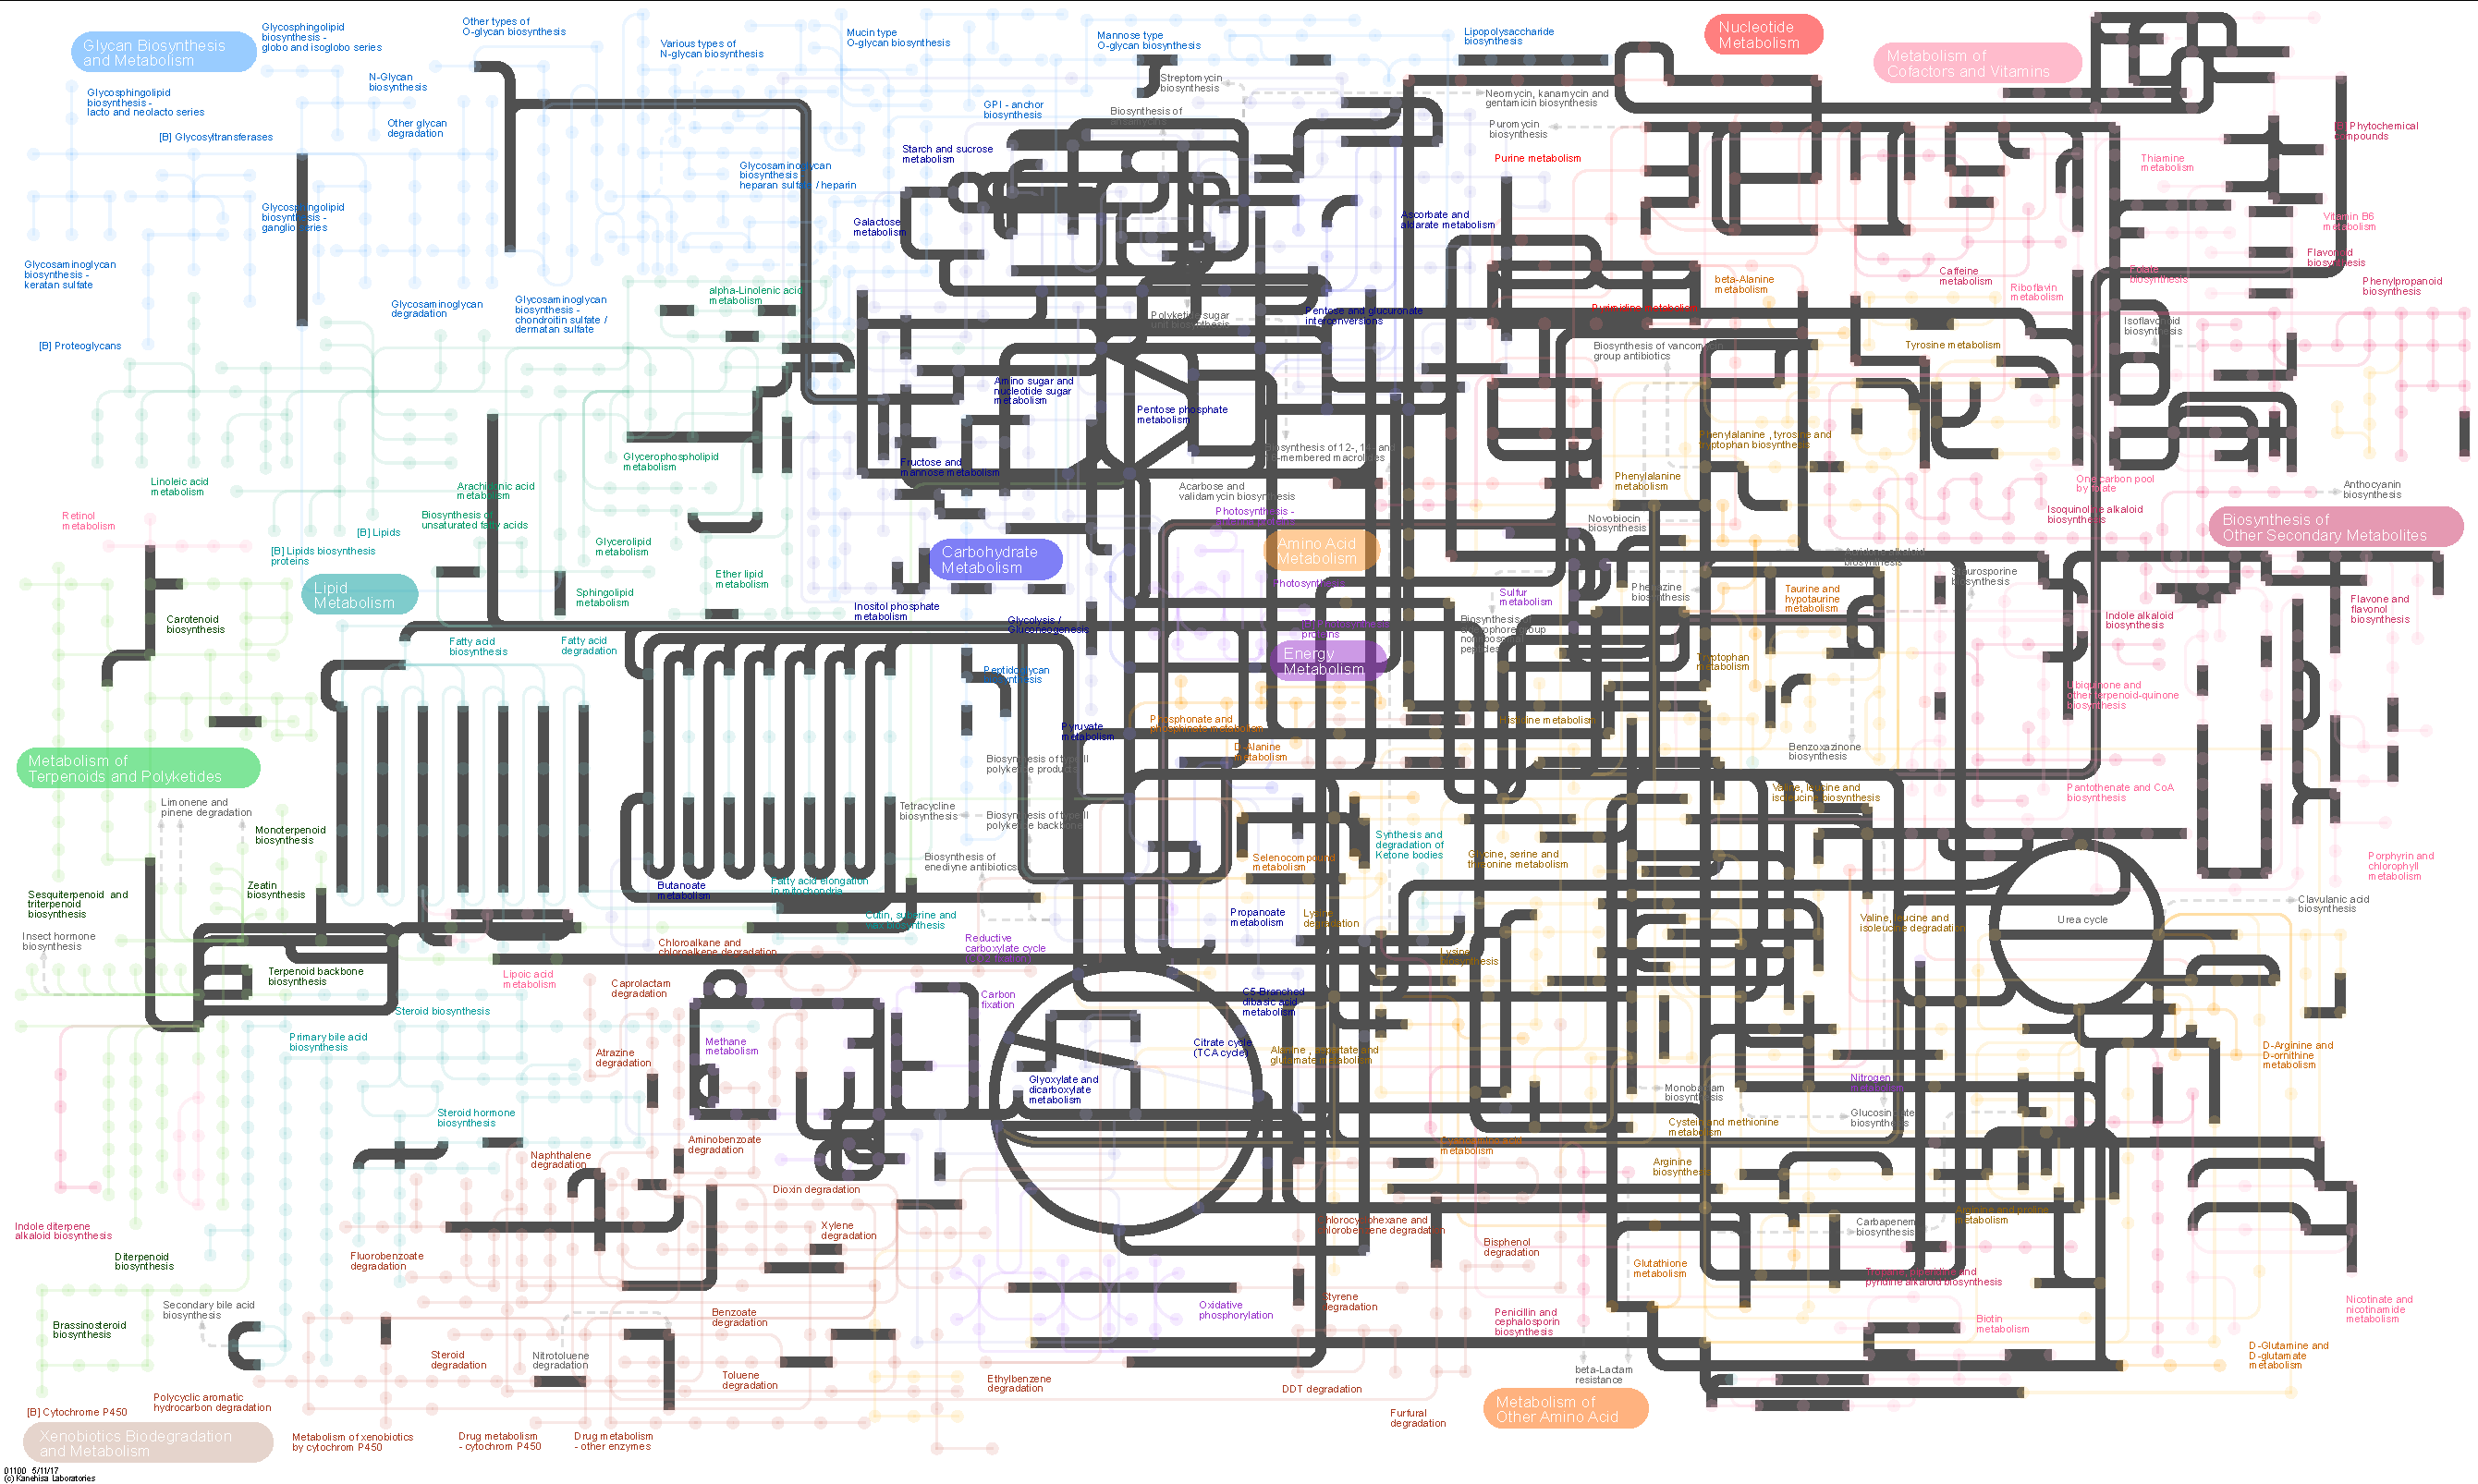
\includegraphics[width=0.95\textwidth]{metabolism/gen_arc_n0.pdf}
    \caption{Reconstruction of LACA's metabolic network from extant life, for the genus-level archaea dataset. In black: enzymes and metabolic pathways that were inferred to be present in LACA.}
    \label{gen4arc_metnet}
\end{figure}   


\begin{figure}[H]
    \centering
    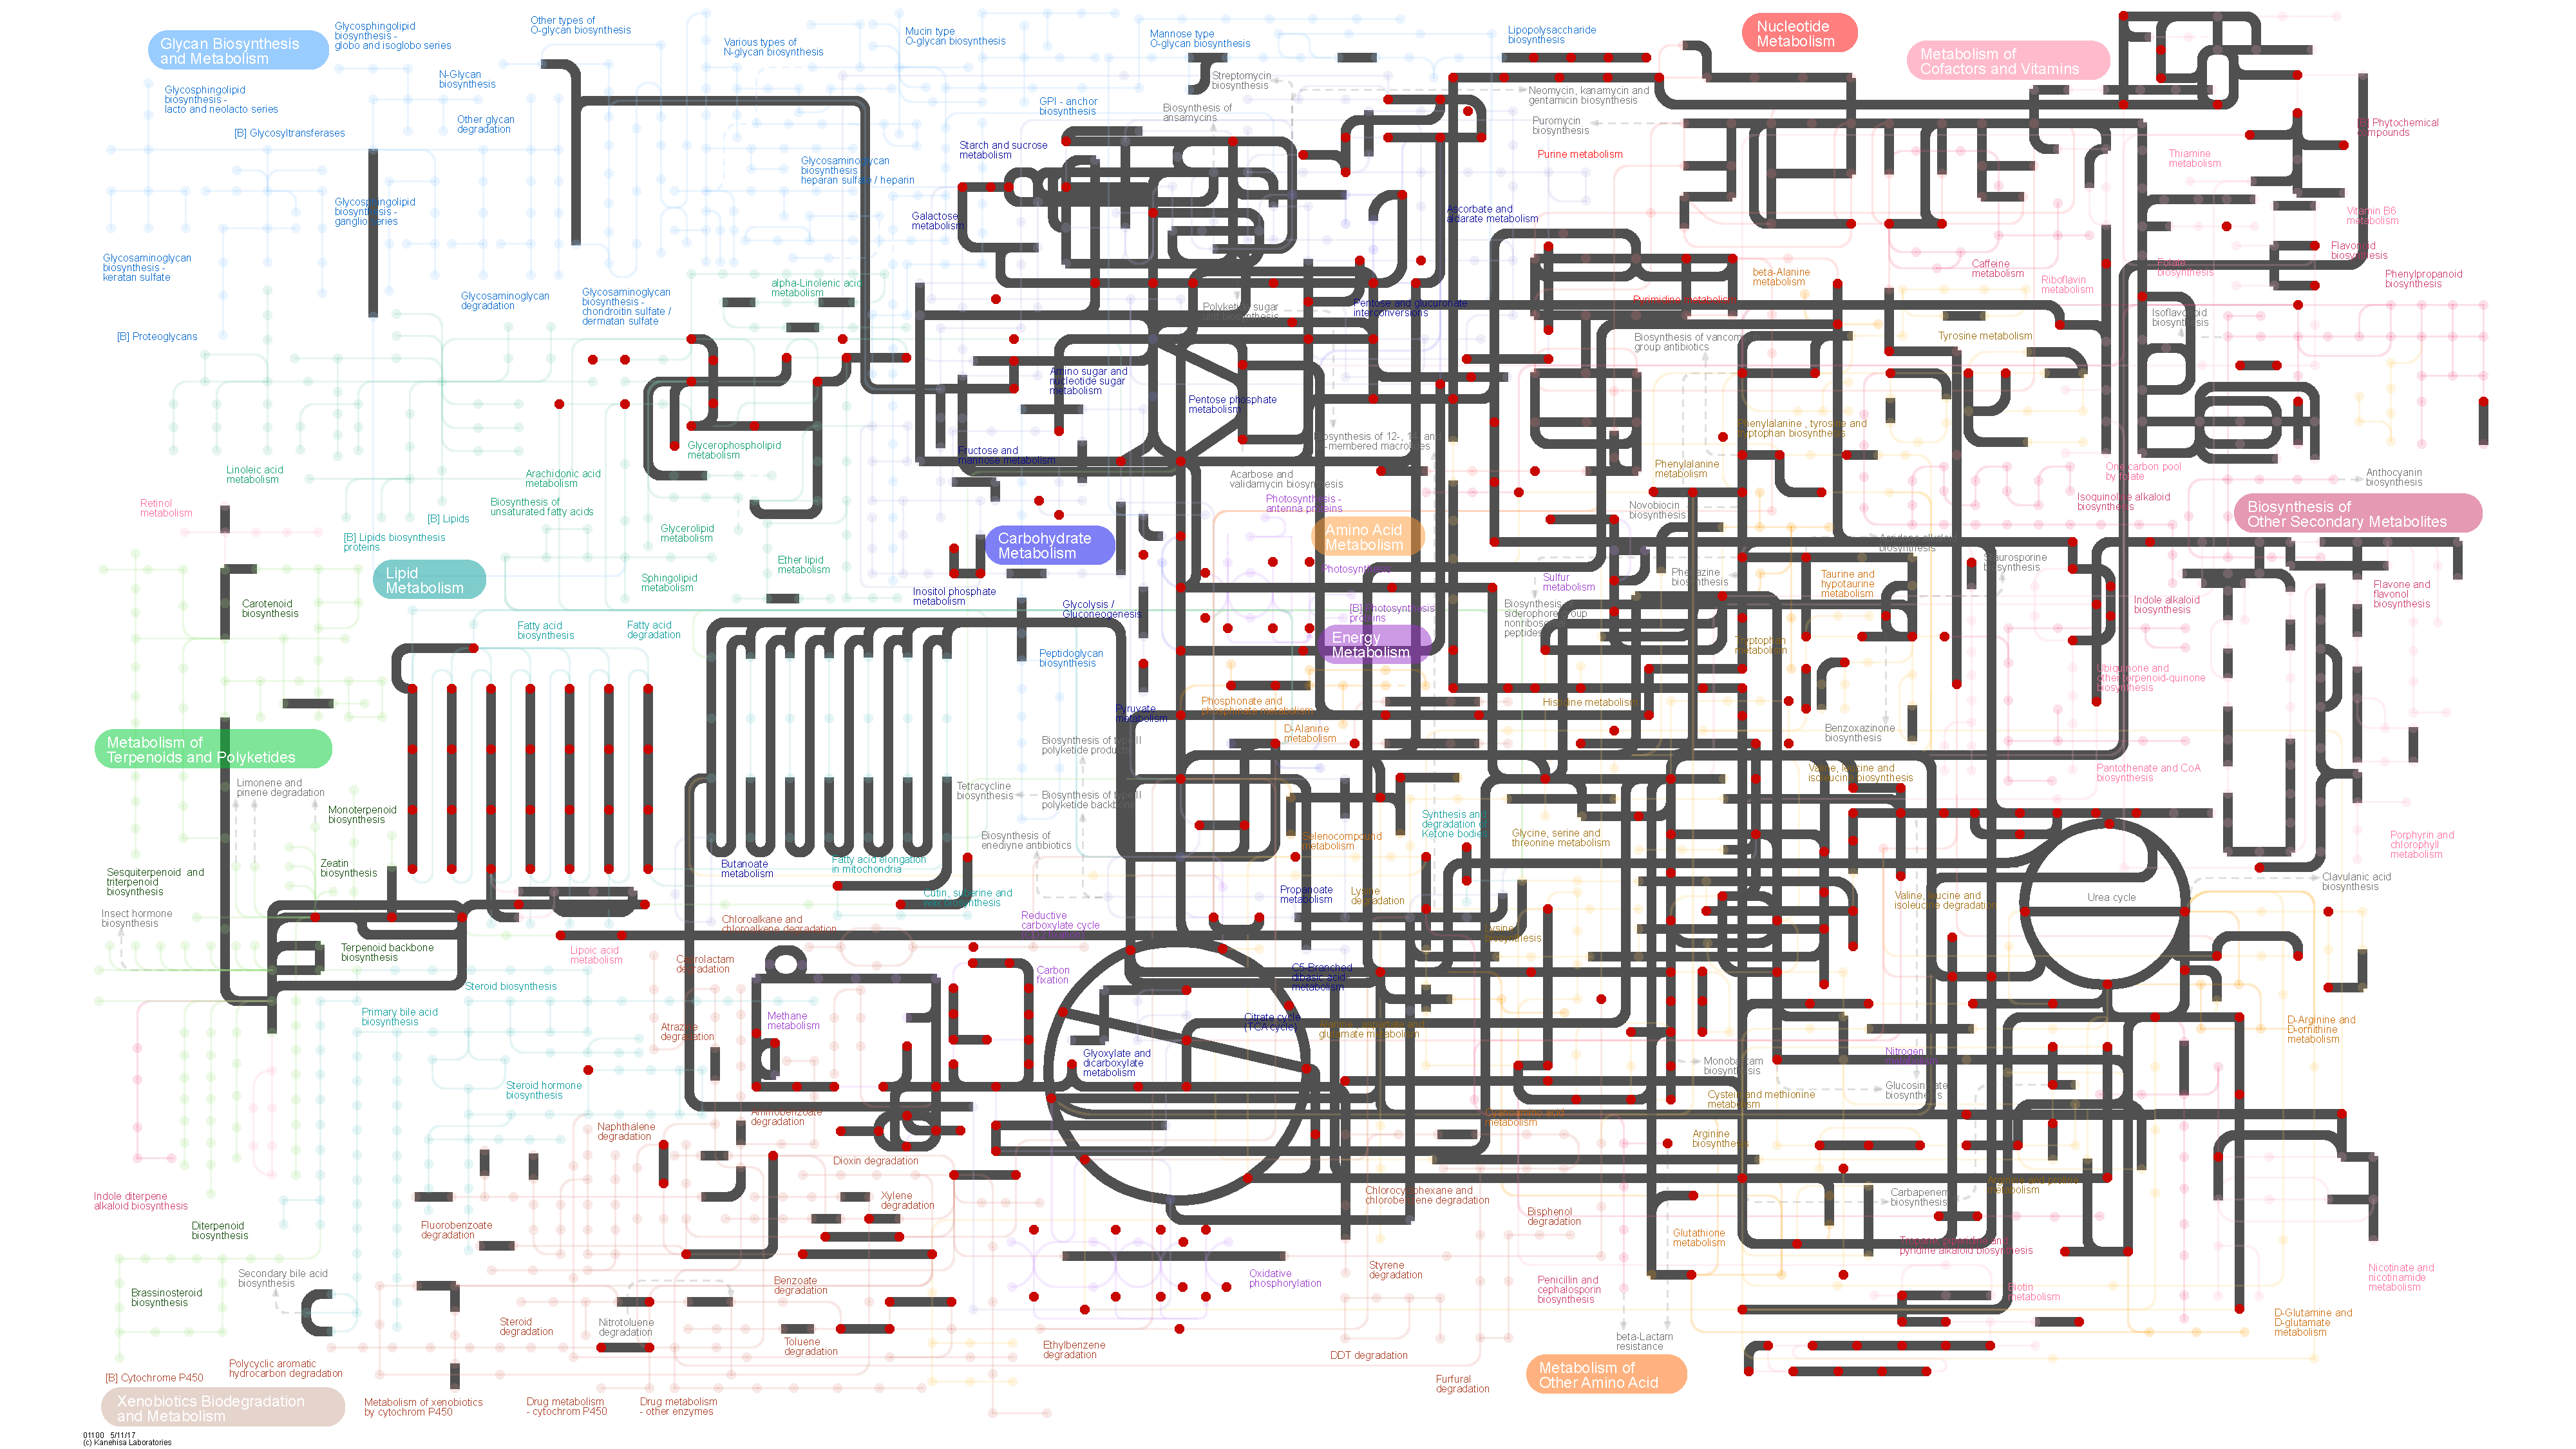
\includegraphics[width=0.95\textwidth]{metabolism/fam_N0_plus_06seedset.pdf}
    \caption{Reconstruction of LACA's metabolic network from extant life, for the family-level archaea dataset. In black: enzymes and metabolic pathways that were inferred to be present in LACA. Red dots: seed compounds of 60\% completeness seed set.}
    \label{fam4arc_metnet_plus_seedset}
\end{figure}   

\begin{figure}[H]
    \centering
    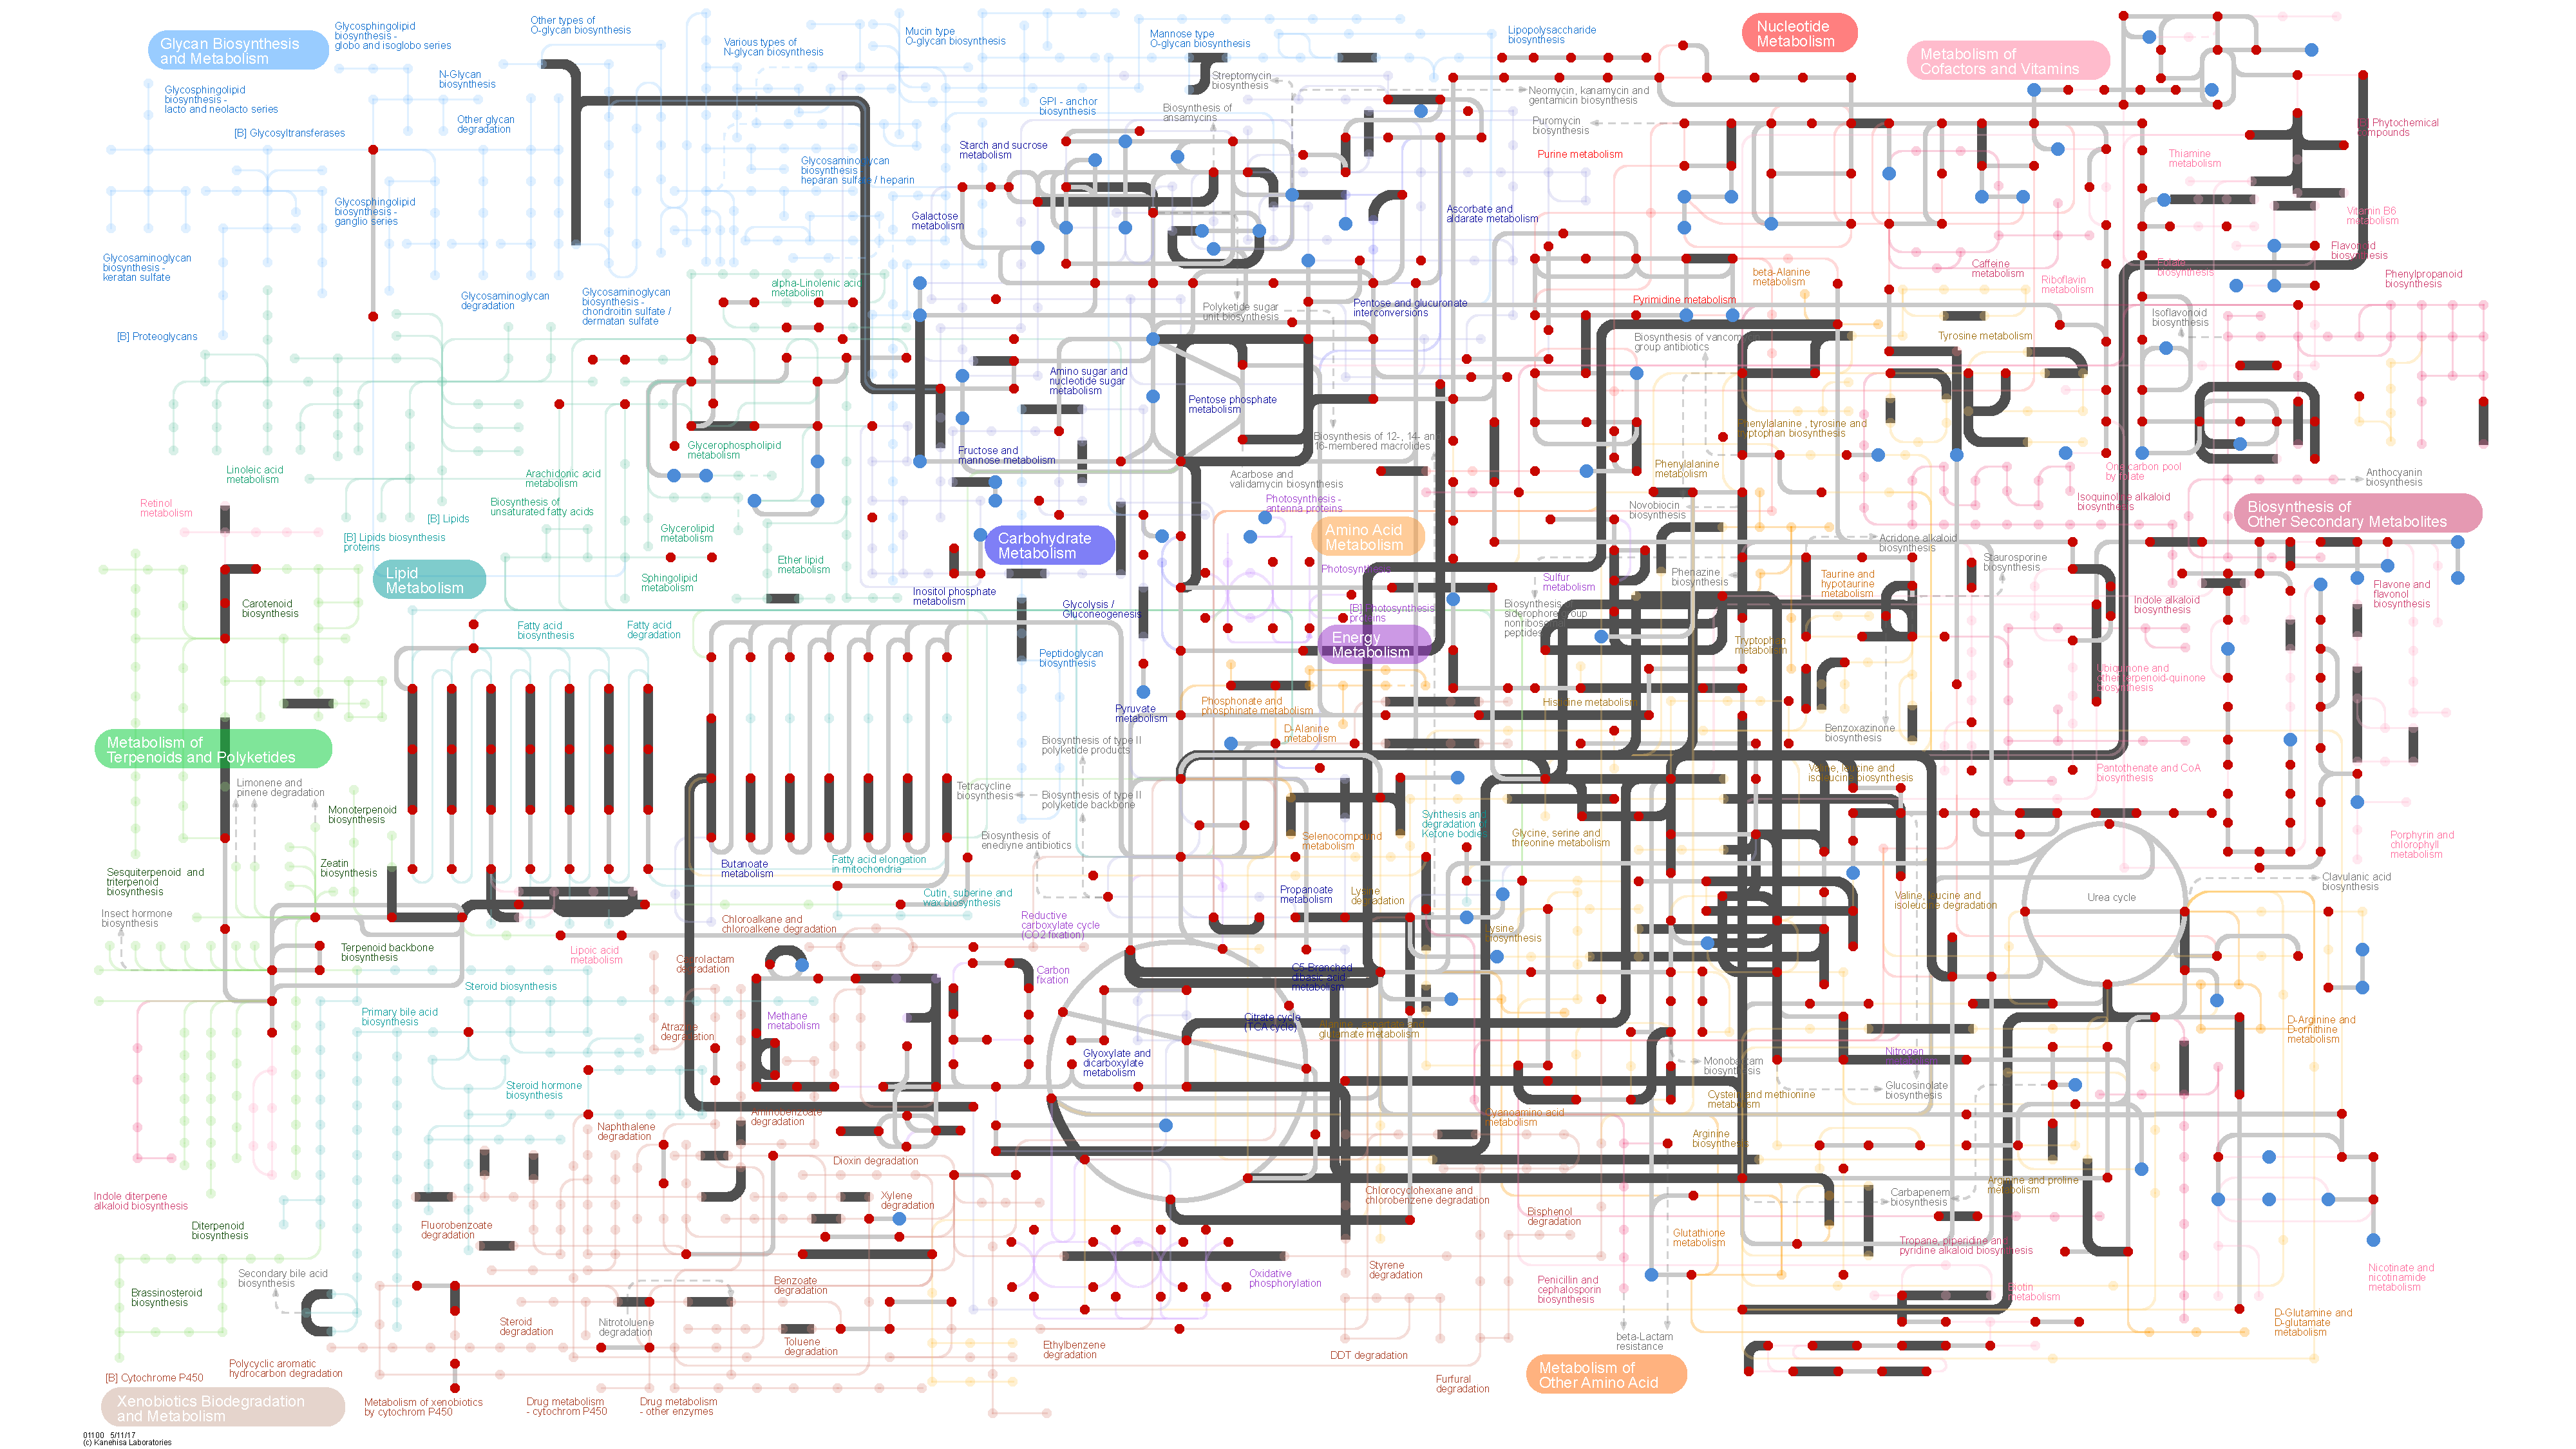
\includegraphics[width=0.98\textwidth]{metabolism/fam_N0_exp1.pdf}
    \caption{Expansion of the archaea family-level reconstructed network of LACA, with the 100\% complexity seed set. In black: enzymes and metabolic pathways that were inferred to be present in LACA, which are not part of the expansion. In gray: enzymes and metabolic pathways of the expanded network. Red dots: respective seed set compounds. Blue dots: scope compounds after network expansion.}    
    \label{fam4arc_metnetexp_1}
\end{figure}

\newpage
\textbf{EC number evolution in LACA.}
\begin{figure}[H]
    \centering
    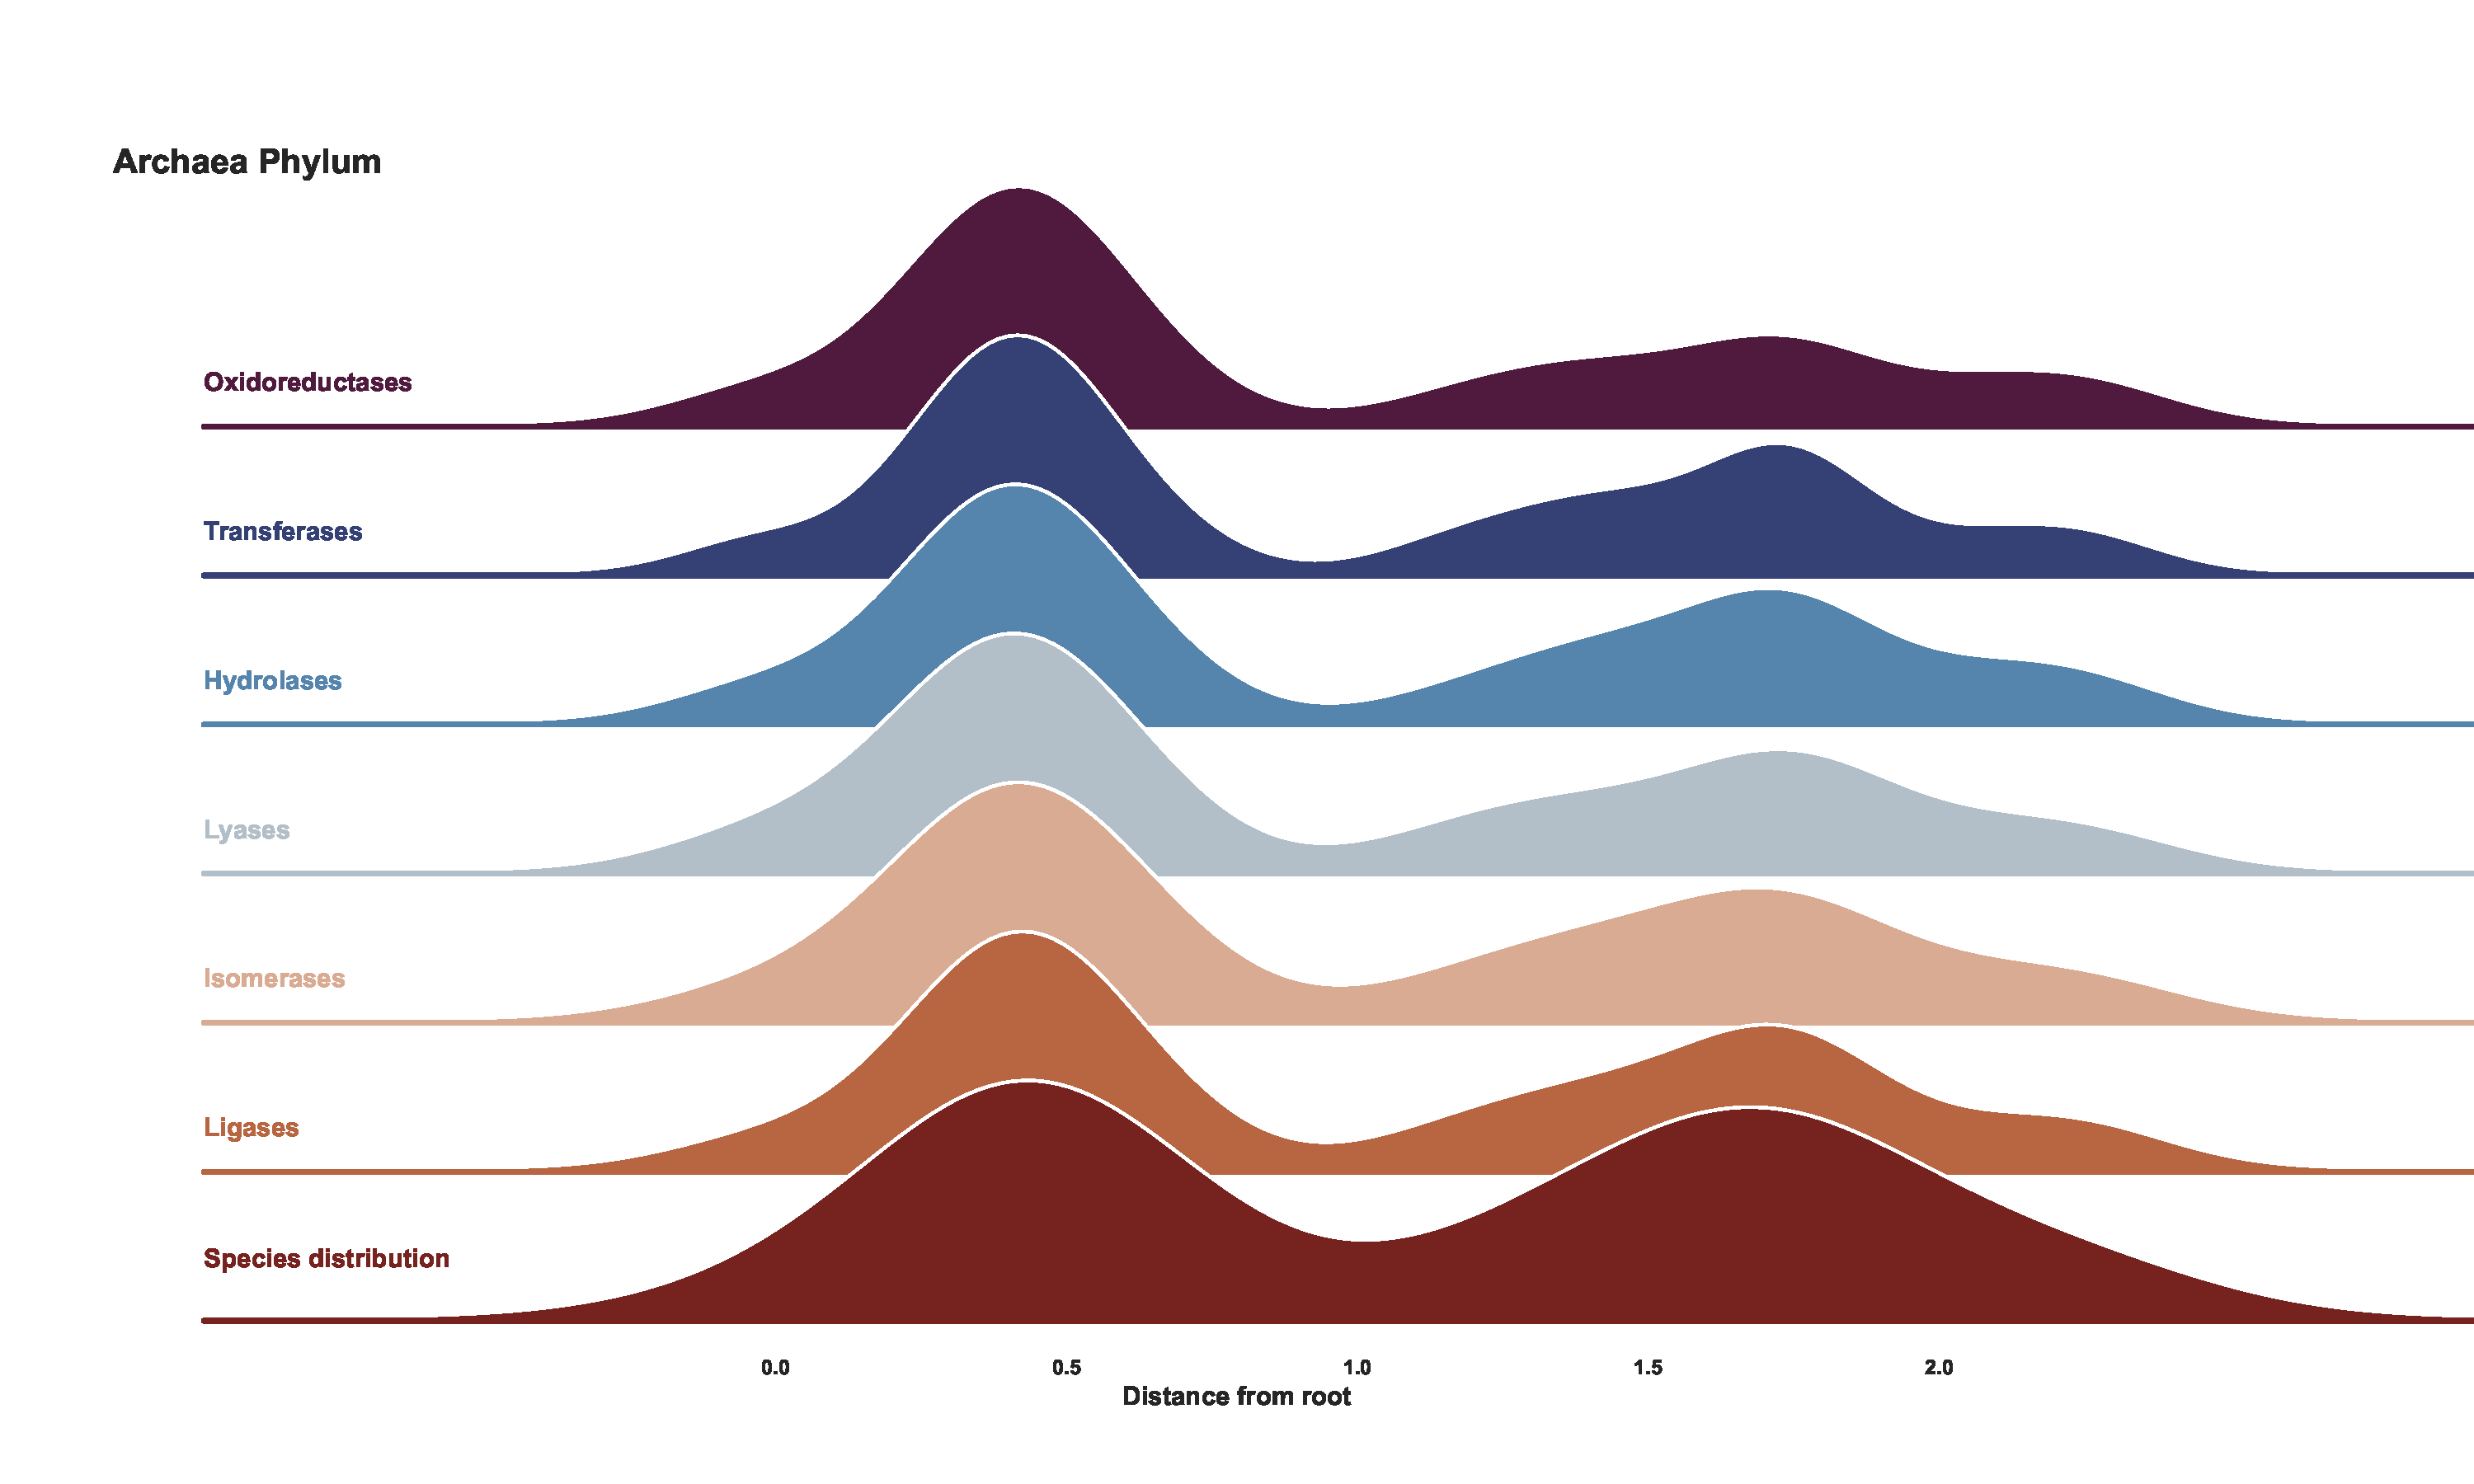
\includegraphics[width=0.95\textwidth]{ridgeplots/phy4arc_ridgeplot.pdf}
    \label{ridgeplot_phy4arc}
\end{figure}

\begin{figure}[H]
    \centering
    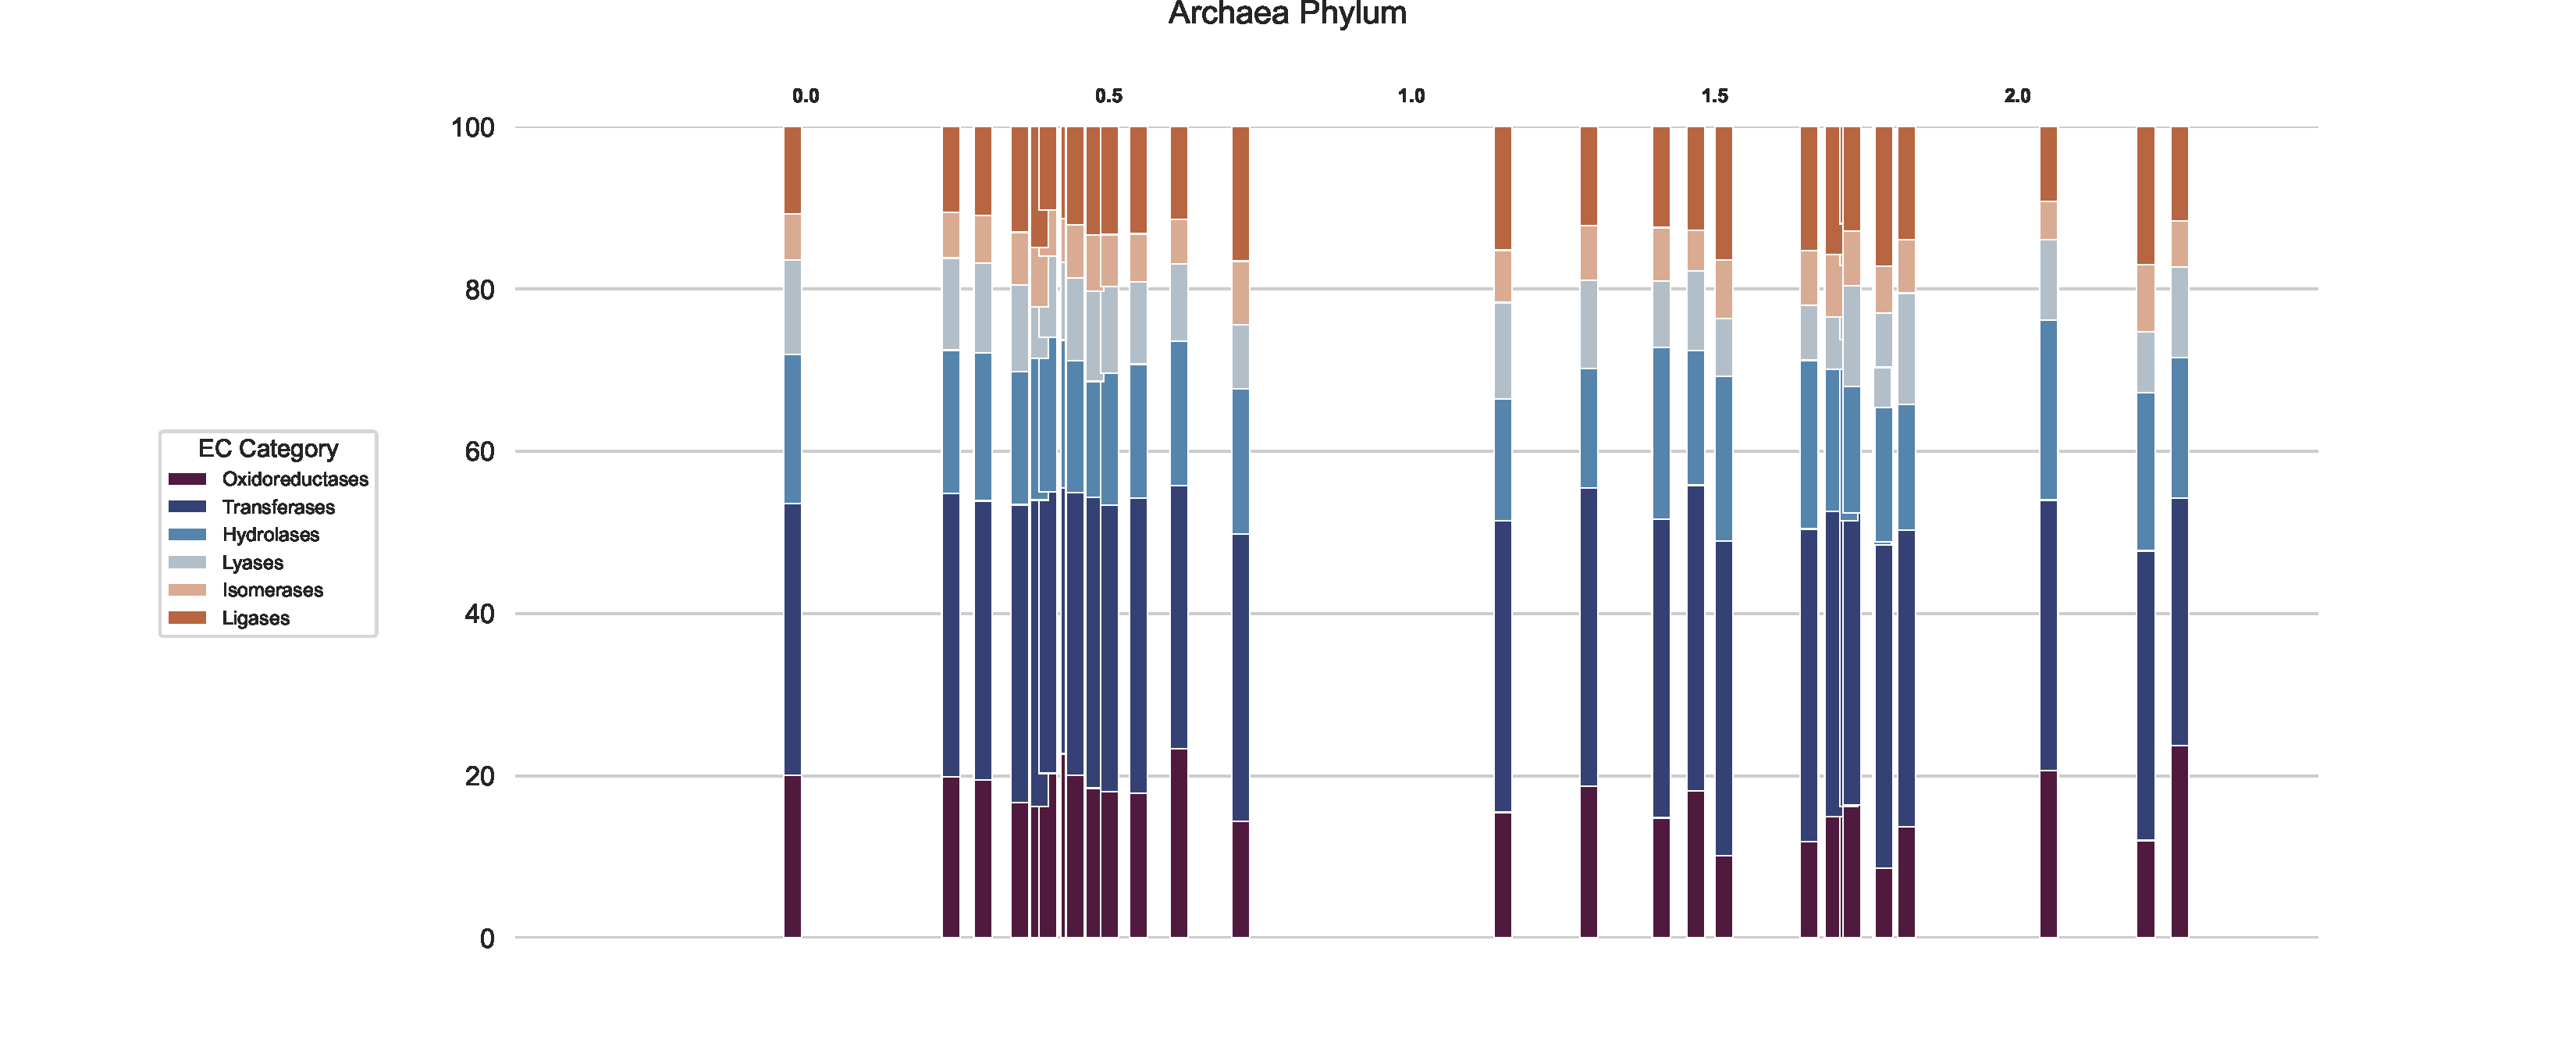
\includegraphics[width=0.95\textwidth]{ridgeplots/phy4arc_barplot.pdf}
    \caption[]{Evolution of individual enzyme categories for the phylum-level archaea dataset. The ridgeplot displays the distribution of each category as a function of distance from the tree root, with the last axis presenting the species distribution, while the barplot the relative abundance of each category at that particular distance as a stacked barplot.}
    \label{barplot_phy4arc}
\end{figure}

\begin{figure}[H]
    \centering
    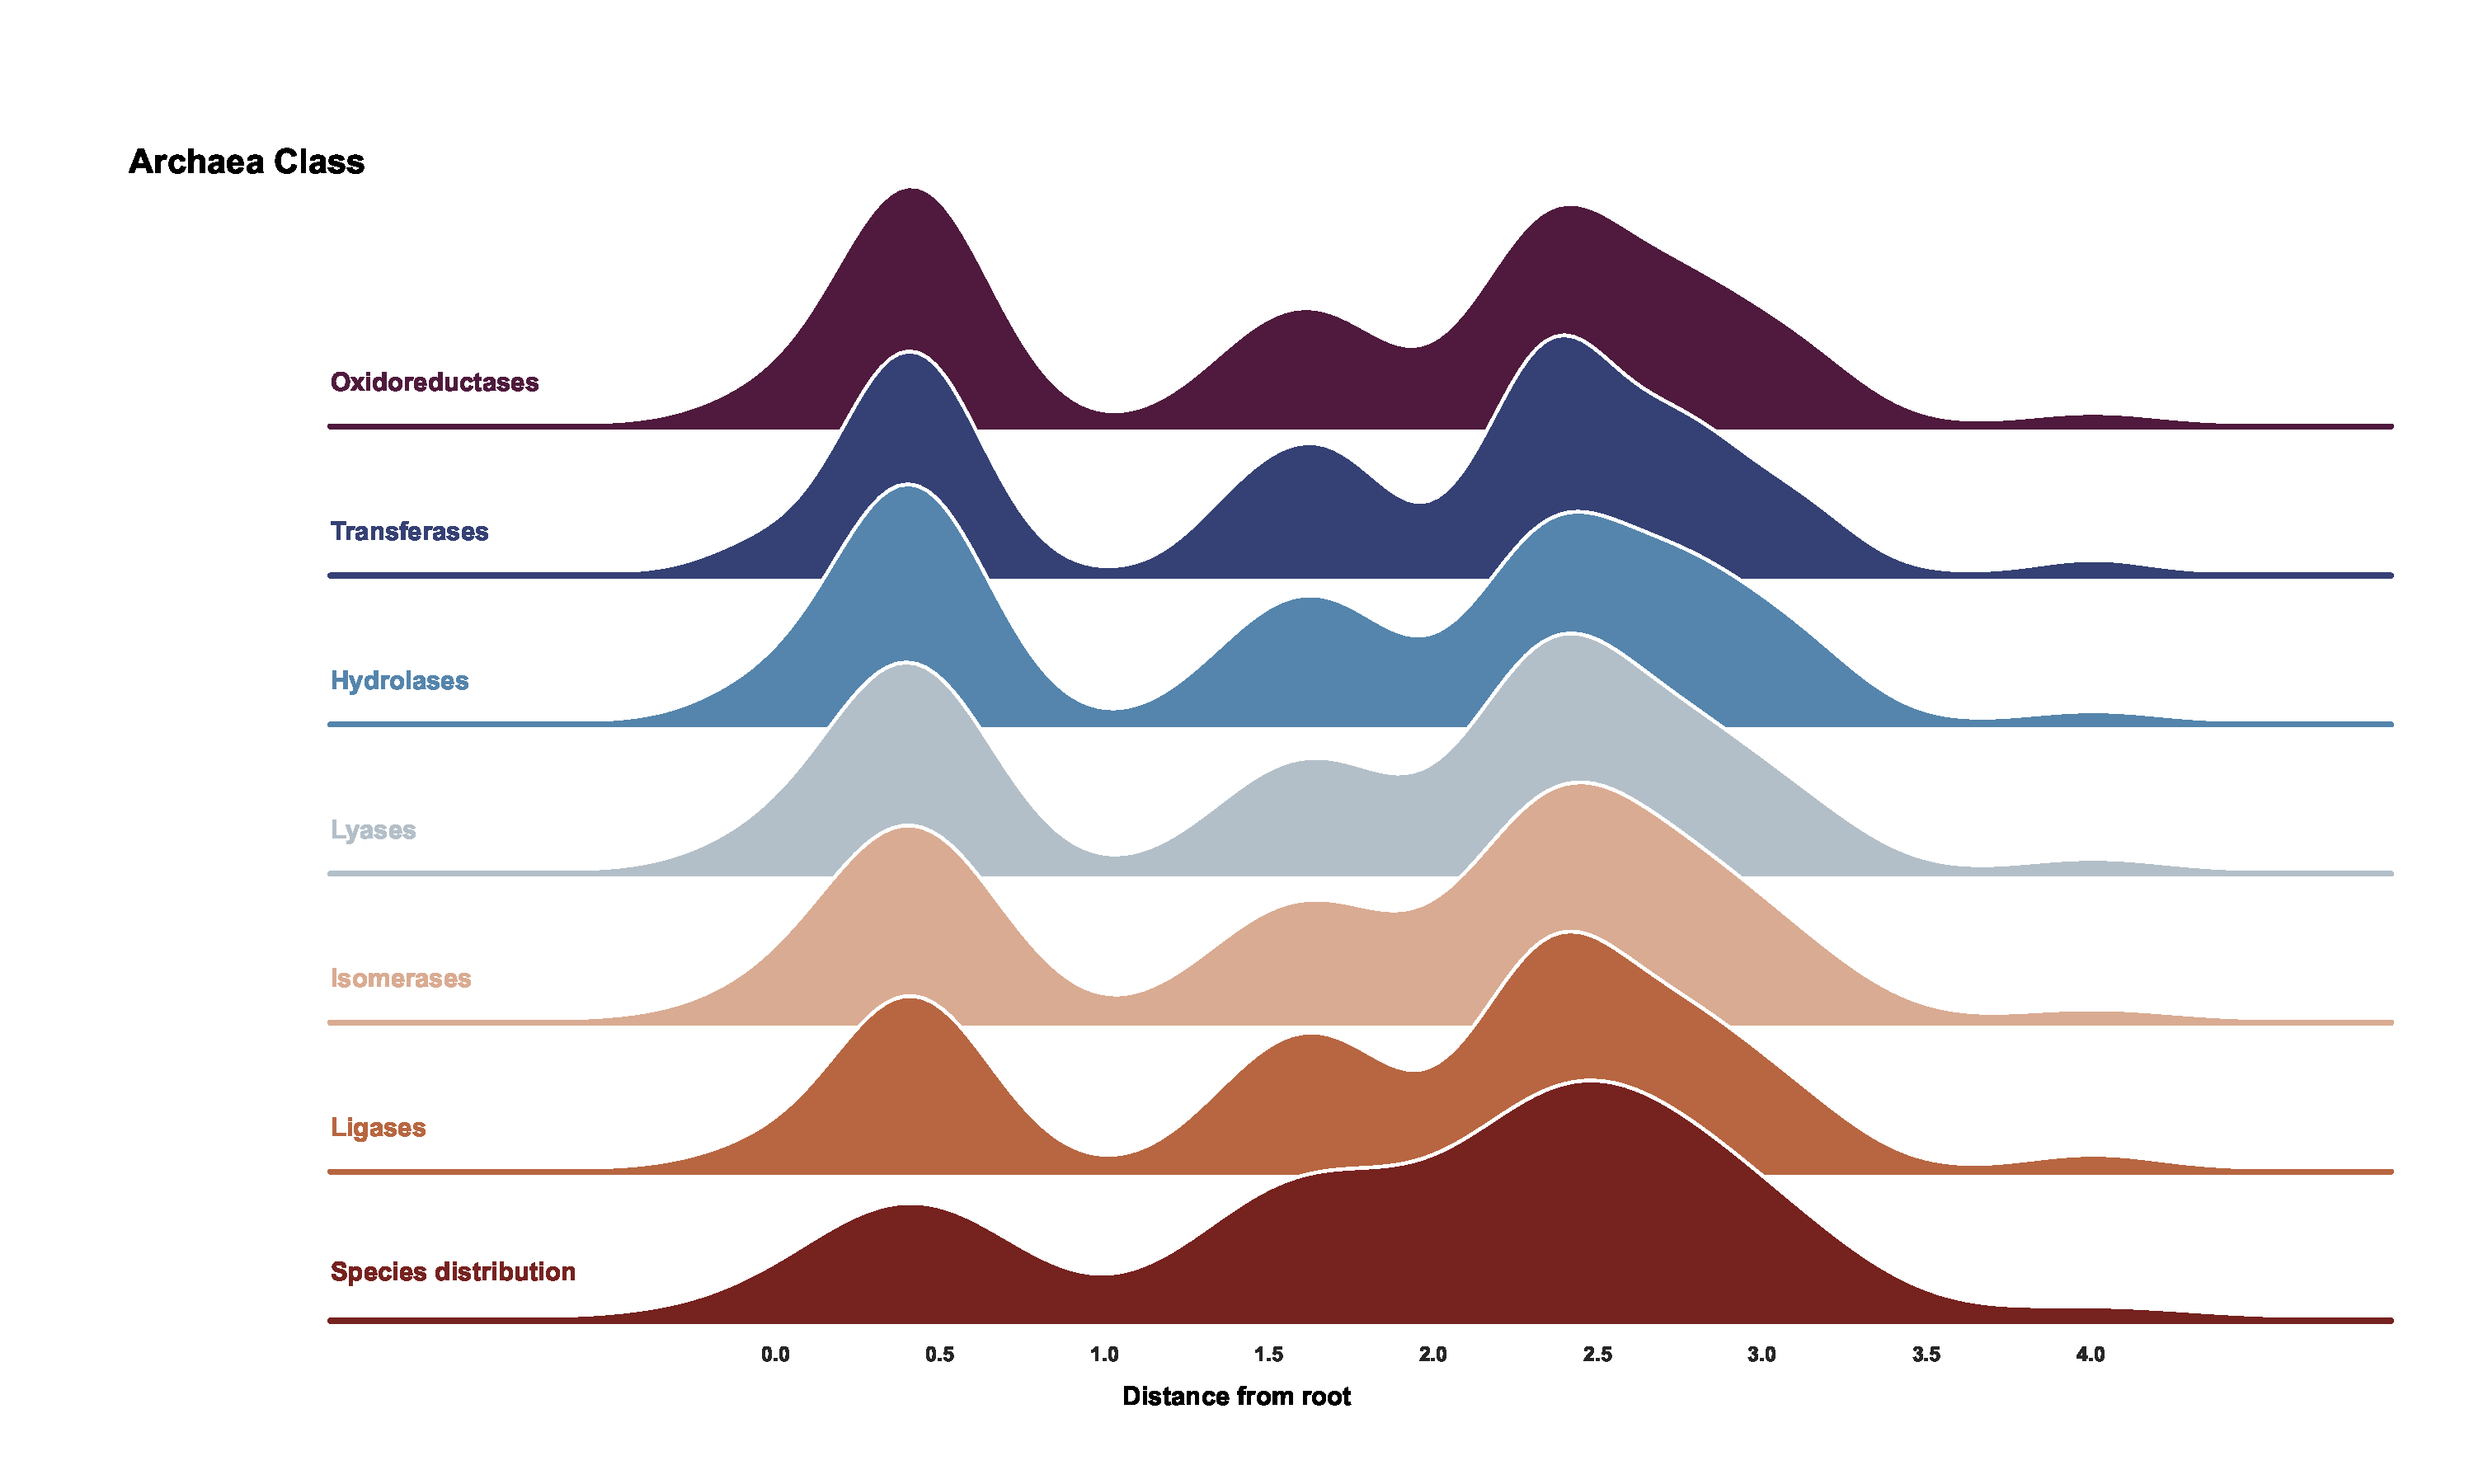
\includegraphics[width=0.95\textwidth]{ridgeplots/cla4arc_ridgeplot.pdf}
    \label{ridgeplot_cla4arc}
\end{figure}

\begin{figure}[H]
    \centering
    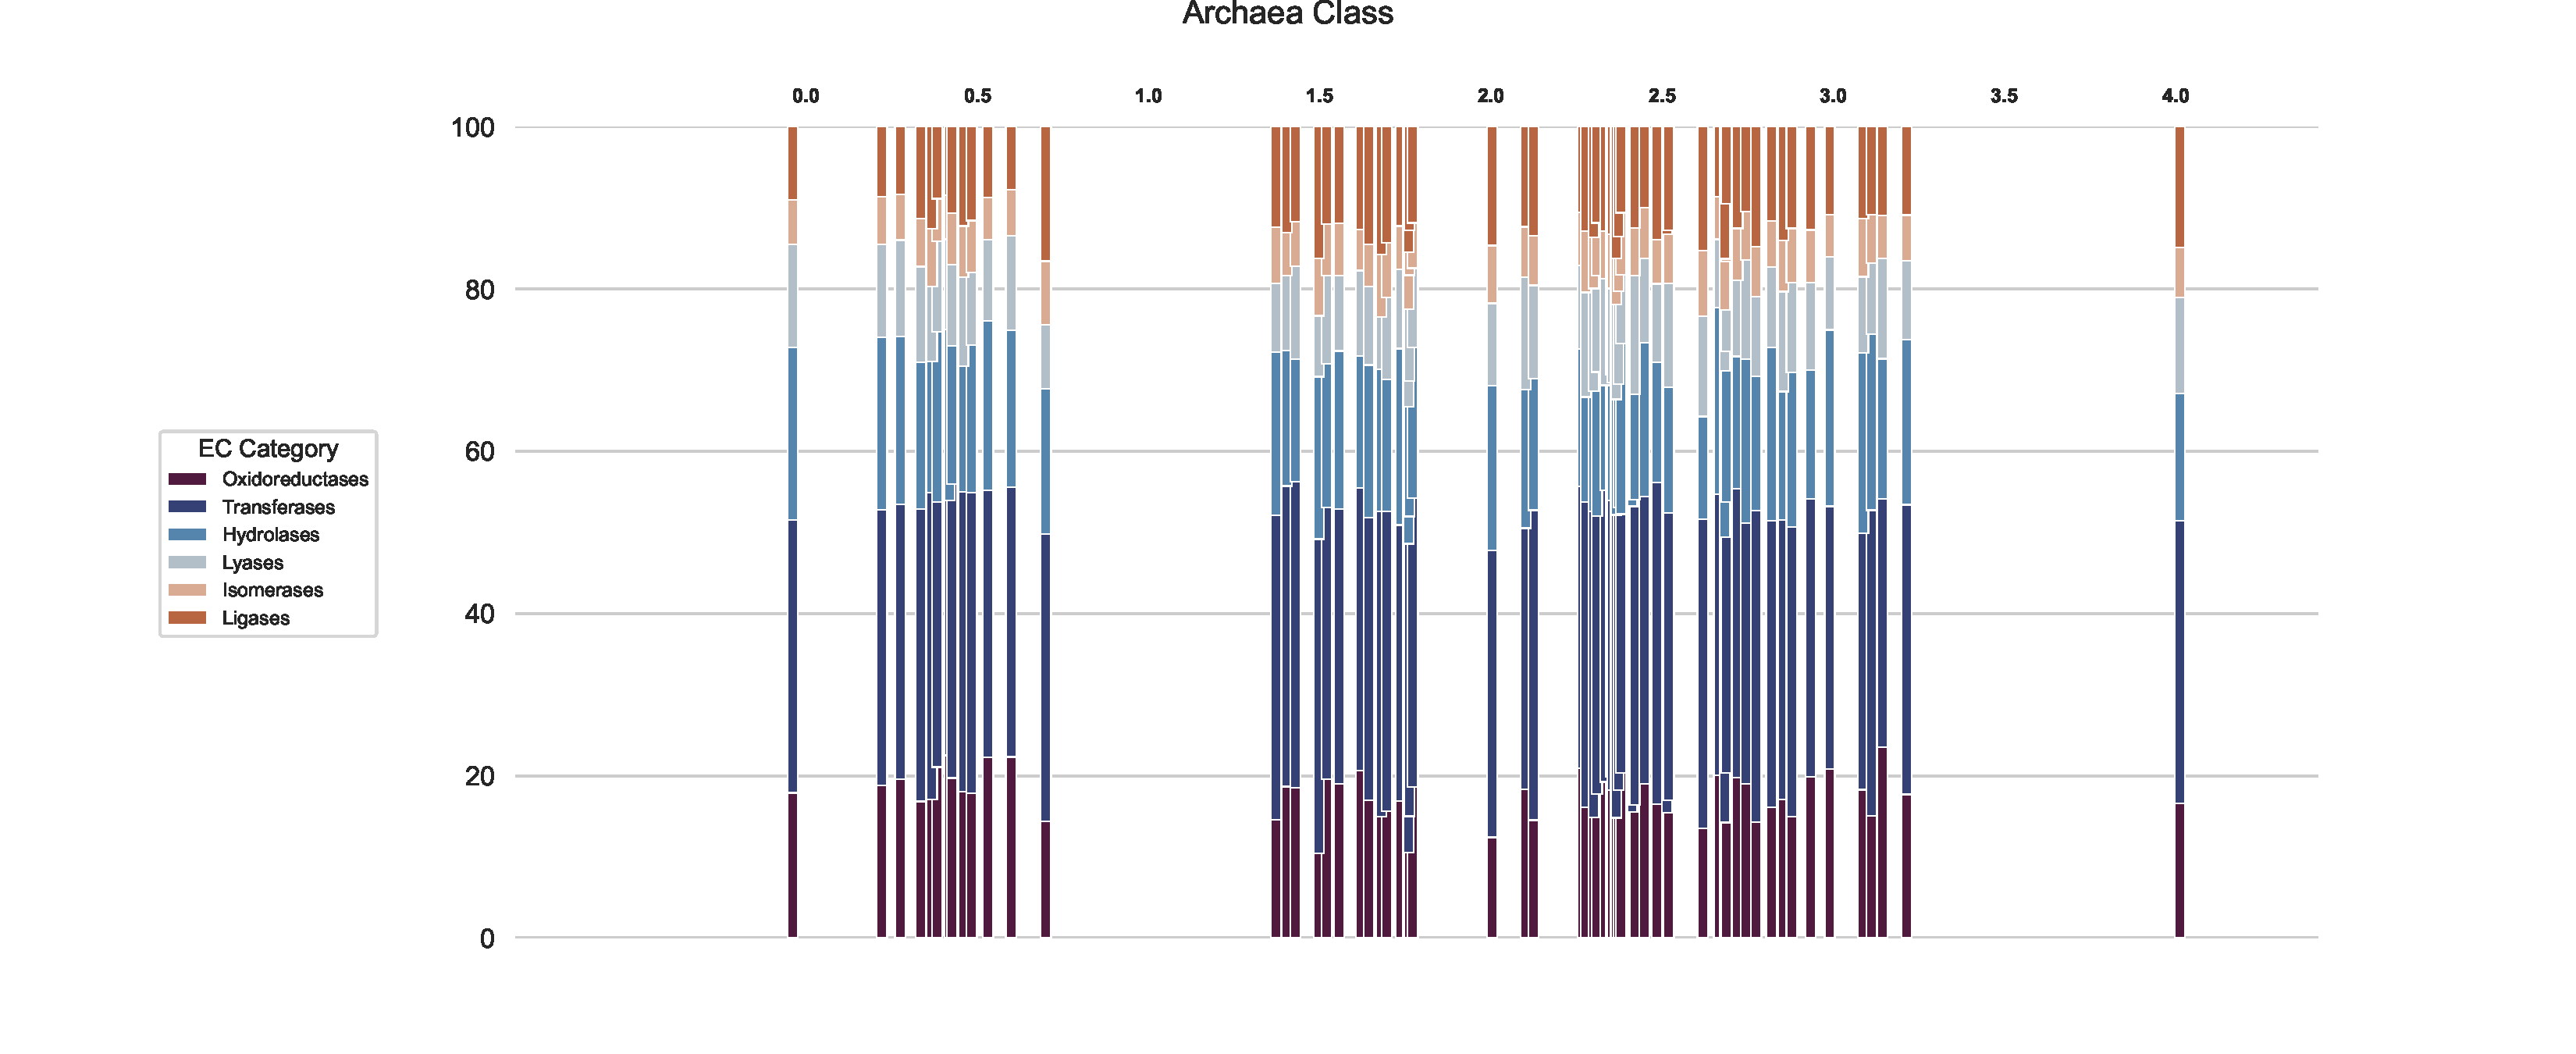
\includegraphics[width=0.95\textwidth]{ridgeplots/cla4arc_barplot.pdf}
    \caption[]{Evolution of individual enzyme categories for the class-level archaea dataset. The ridgeplot displays the distribution of each category as a function of distance from the tree root, with the last axis presenting the species distribution, while the barplot the relative abundance of each category at that particular distance as a stacked barplot.}
    \label{barplot_cla4arc}
\end{figure}

\begin{figure}[H]
    \centering
    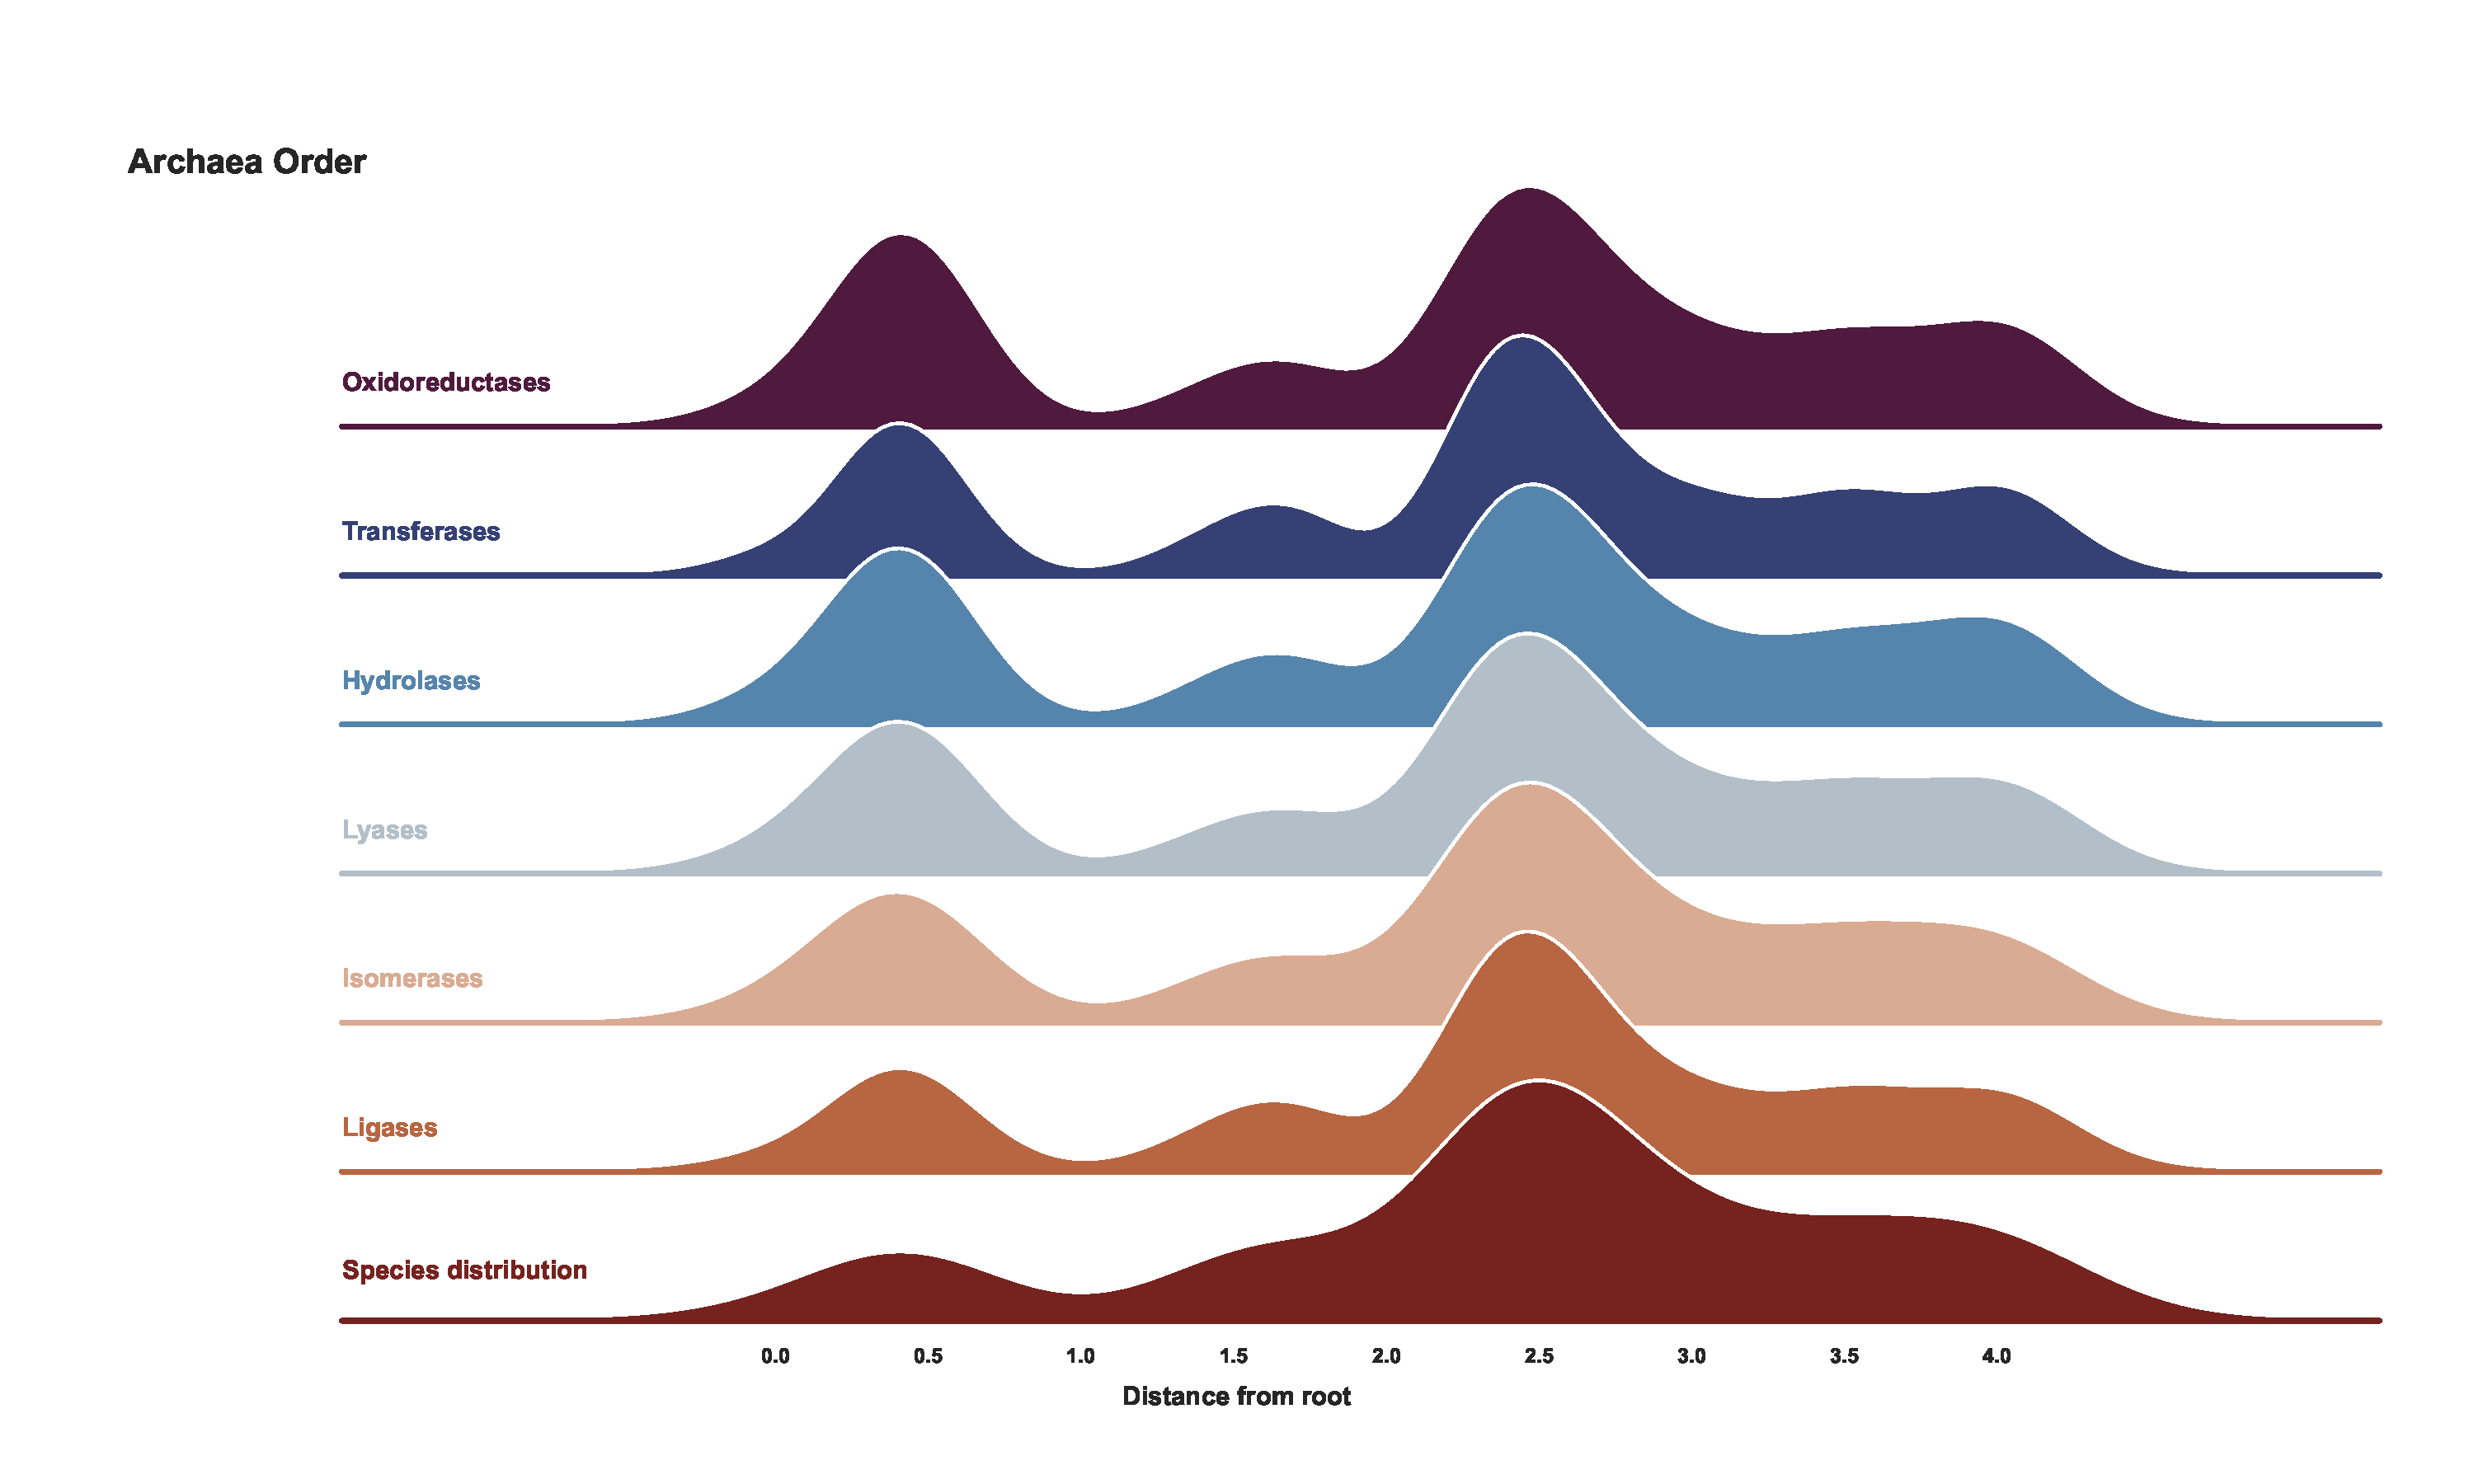
\includegraphics[width=0.95\textwidth]{ridgeplots/ord4arc_ridgeplot.pdf}
    \label{ridgeplot_ord4arc}
\end{figure}

\begin{figure}[H]
    \centering
    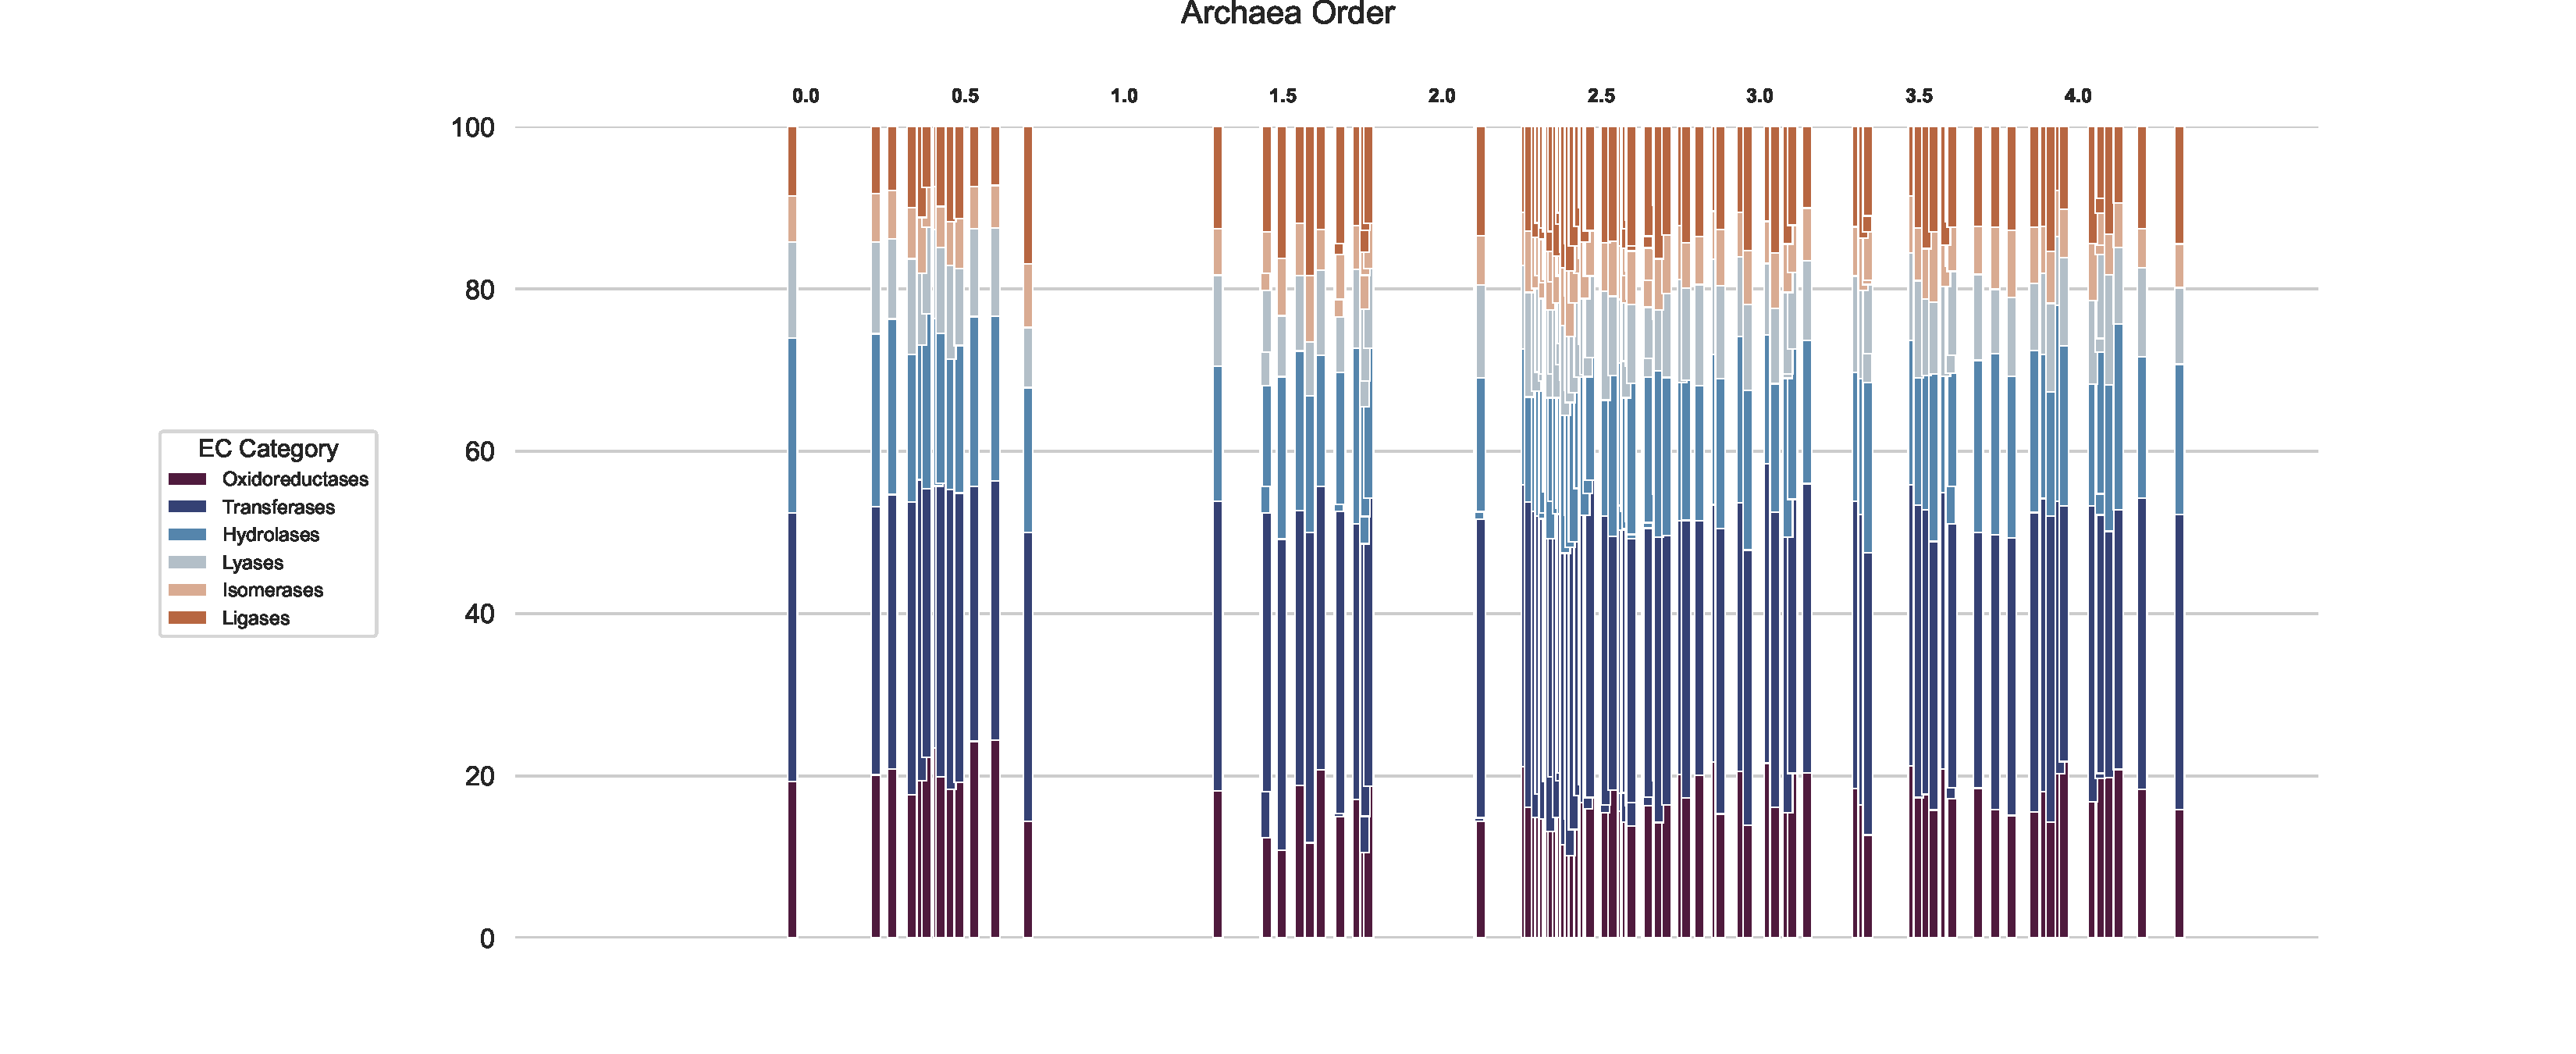
\includegraphics[width=0.95\textwidth]{ridgeplots/ord4arc_barplot.pdf}
    \caption[]{Evolution of individual enzyme categories for the order-level archaea dataset. The ridgeplot displays the distribution of each category as a function of distance from the tree root, with the last axis presenting the species distribution, while the barplot the relative abundance of each category at that particular distance as a stacked barplot.}
    \label{barplot_ord4arc}
\end{figure}

\begin{figure}[H]
    \centering
    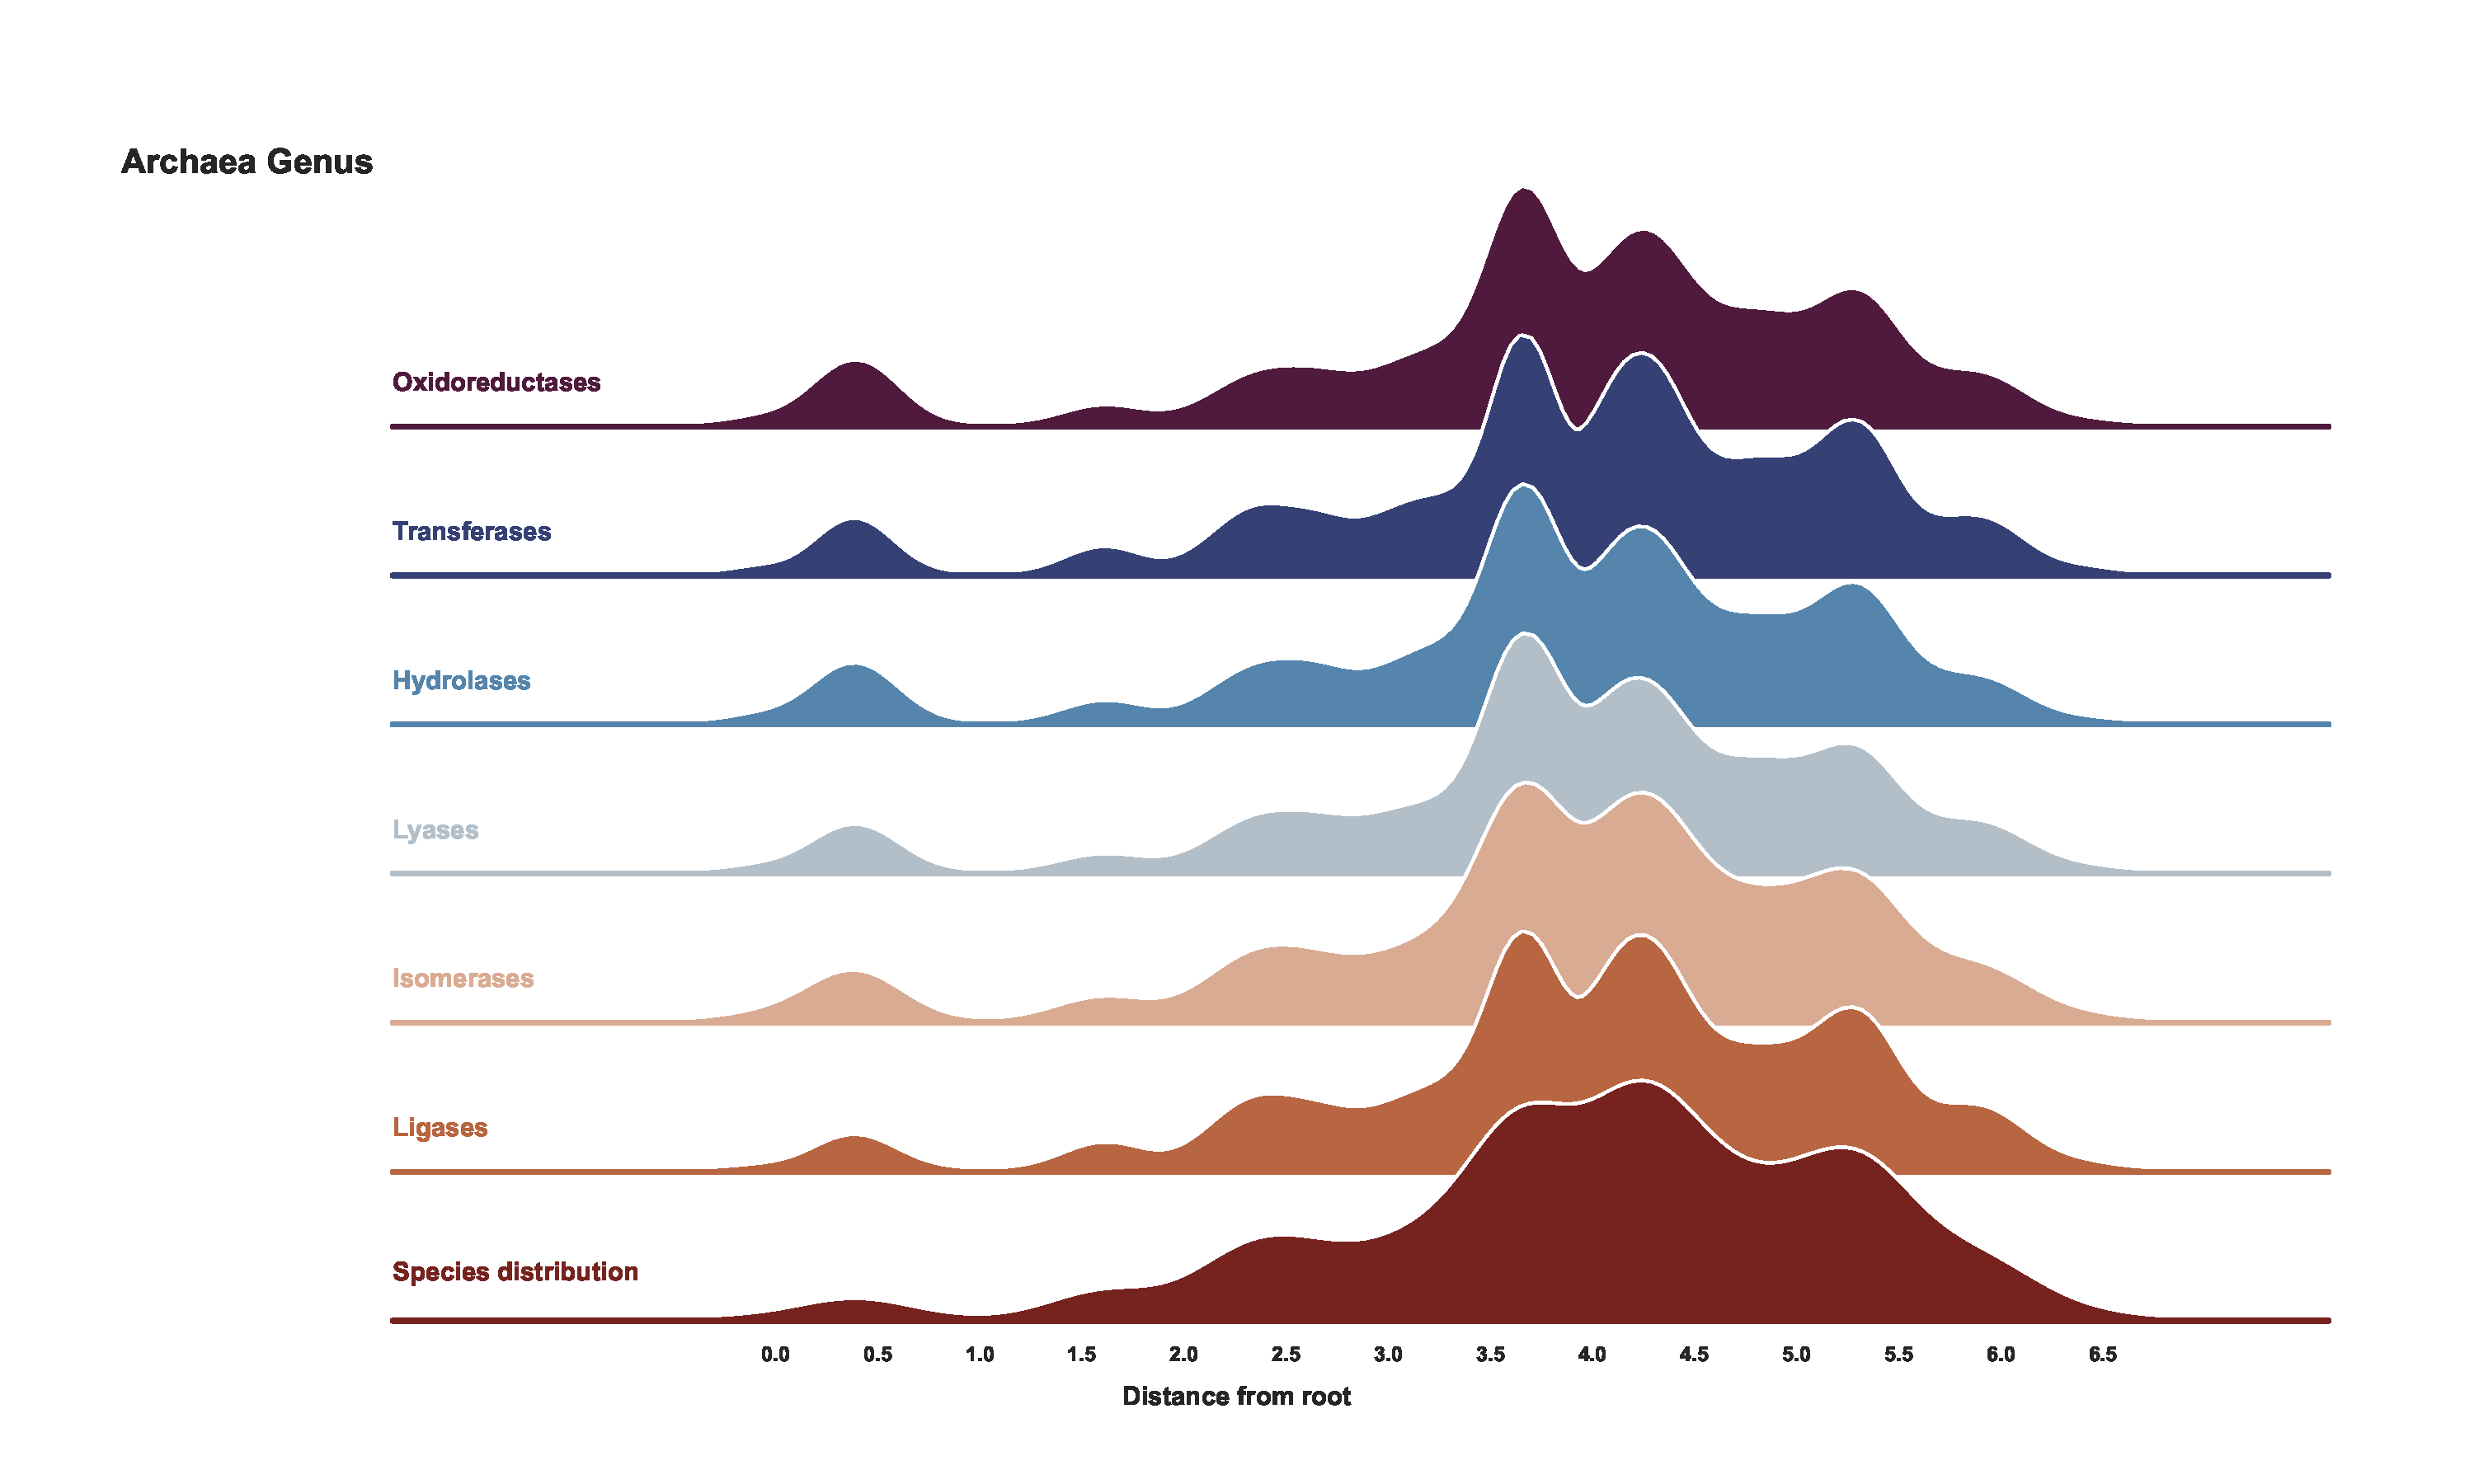
\includegraphics[width=0.95\textwidth]{ridgeplots/gen4arc_ridgeplot.pdf}
    \label{ridgeplot_gen4arc}
\end{figure}

\begin{figure}[H]
    \centering
    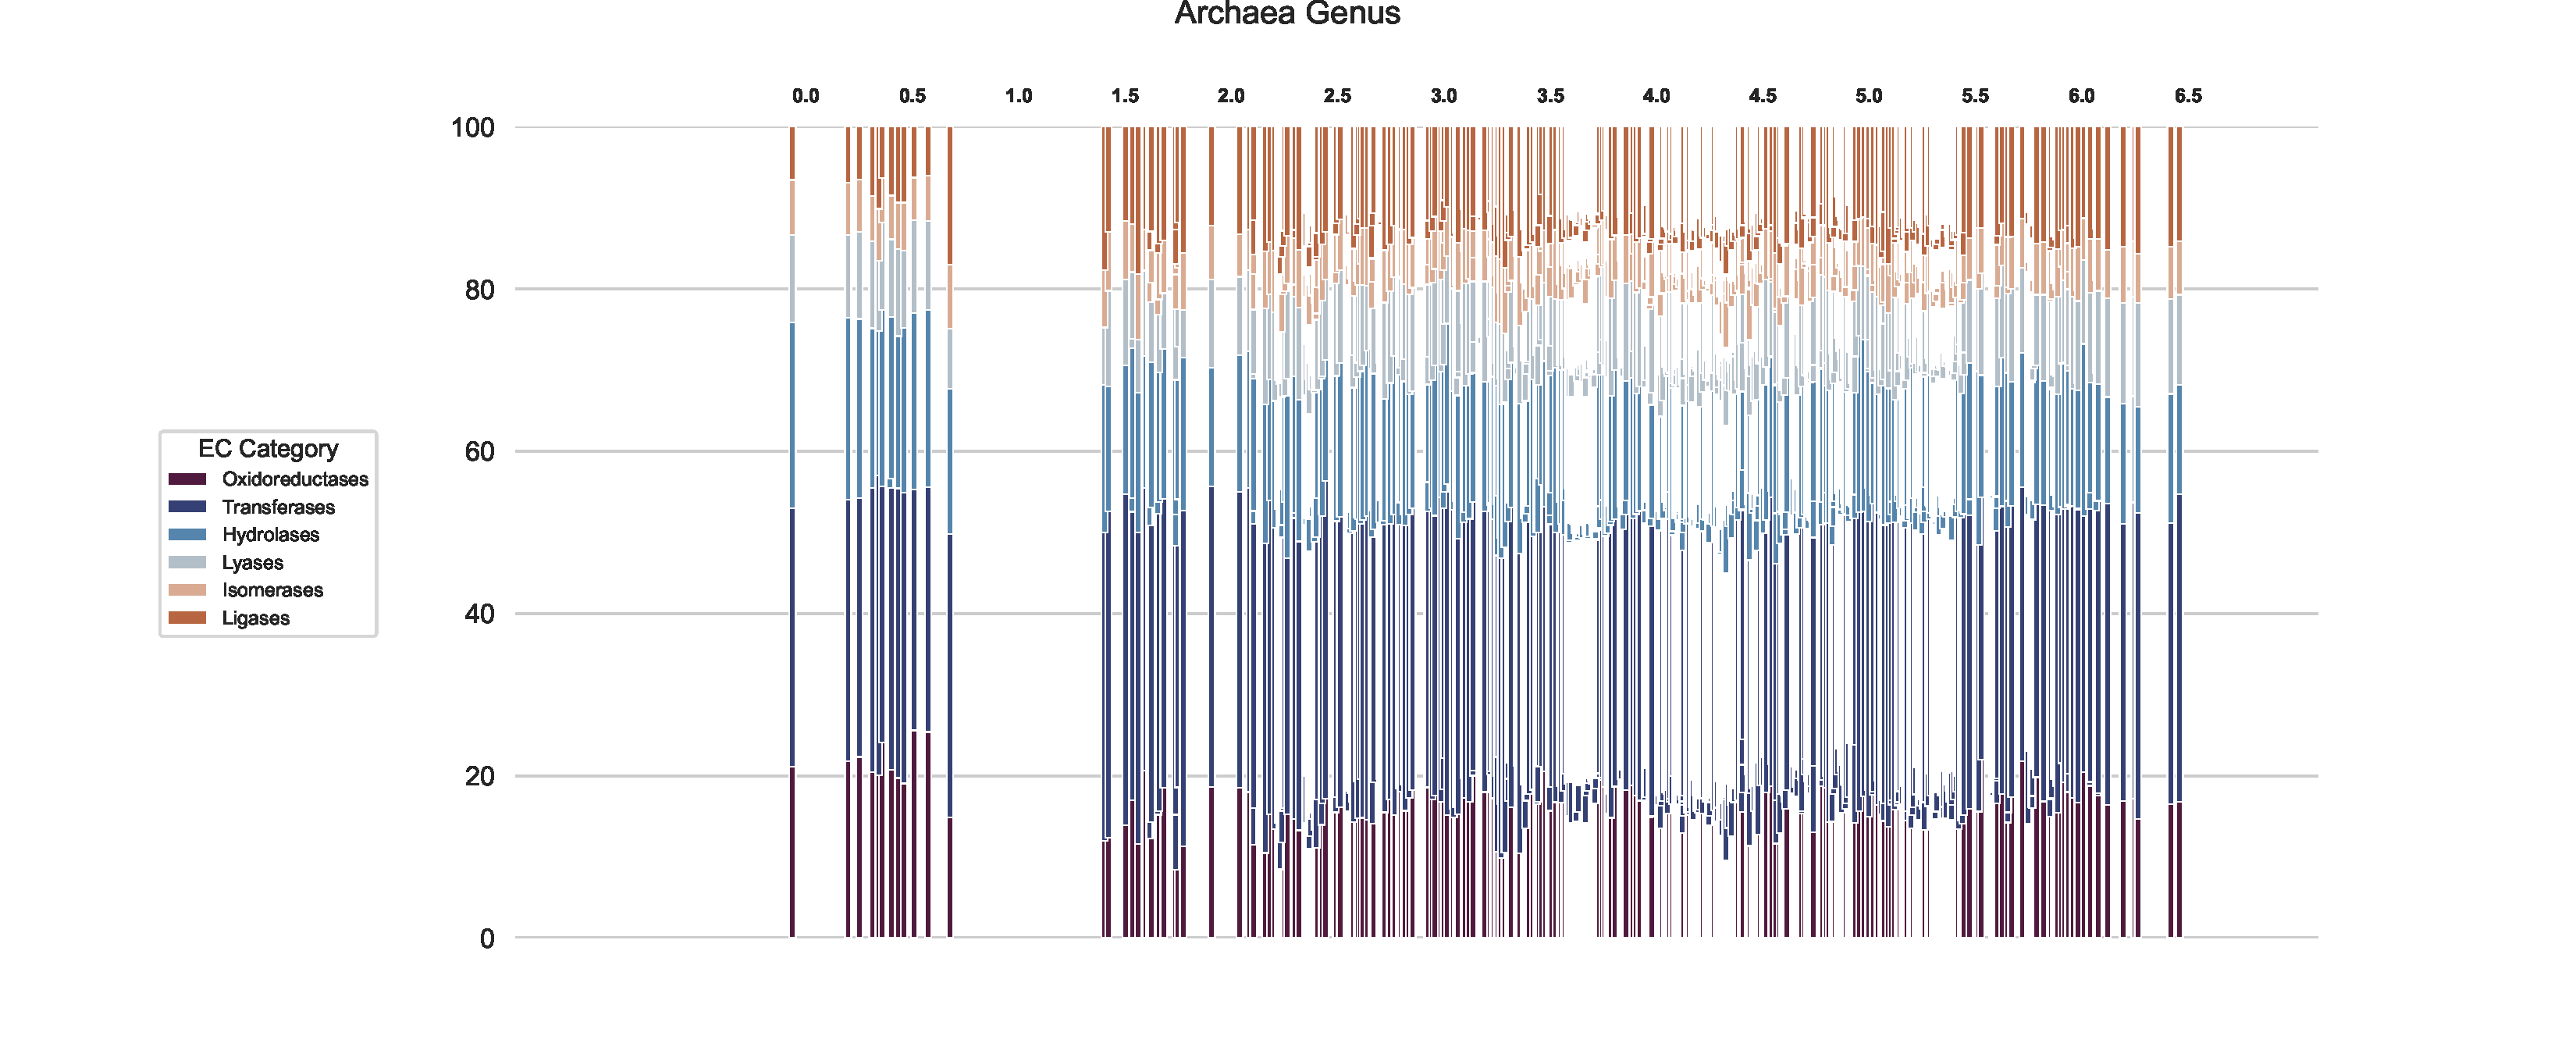
\includegraphics[width=0.95\textwidth]{ridgeplots/gen4arc_barplot.pdf}
    \caption[]{Evolution of individual enzyme categories for the genus-level archaea dataset. The ridgeplot displays the distribution of each category as a function of distance from the tree root, with the last axis presenting the species distribution, while the barplot the relative abundance of each category at that particular distance as a stacked barplot.}
    \label{barplot_gen4arc}
\end{figure}


\newpage
\subsection*{A3. Expansion Scope Size as a Function of Distance to Root}
\textbf{For every taxonomic level dataset, per seed set.}

\begin{figure}[H]
    \centering
    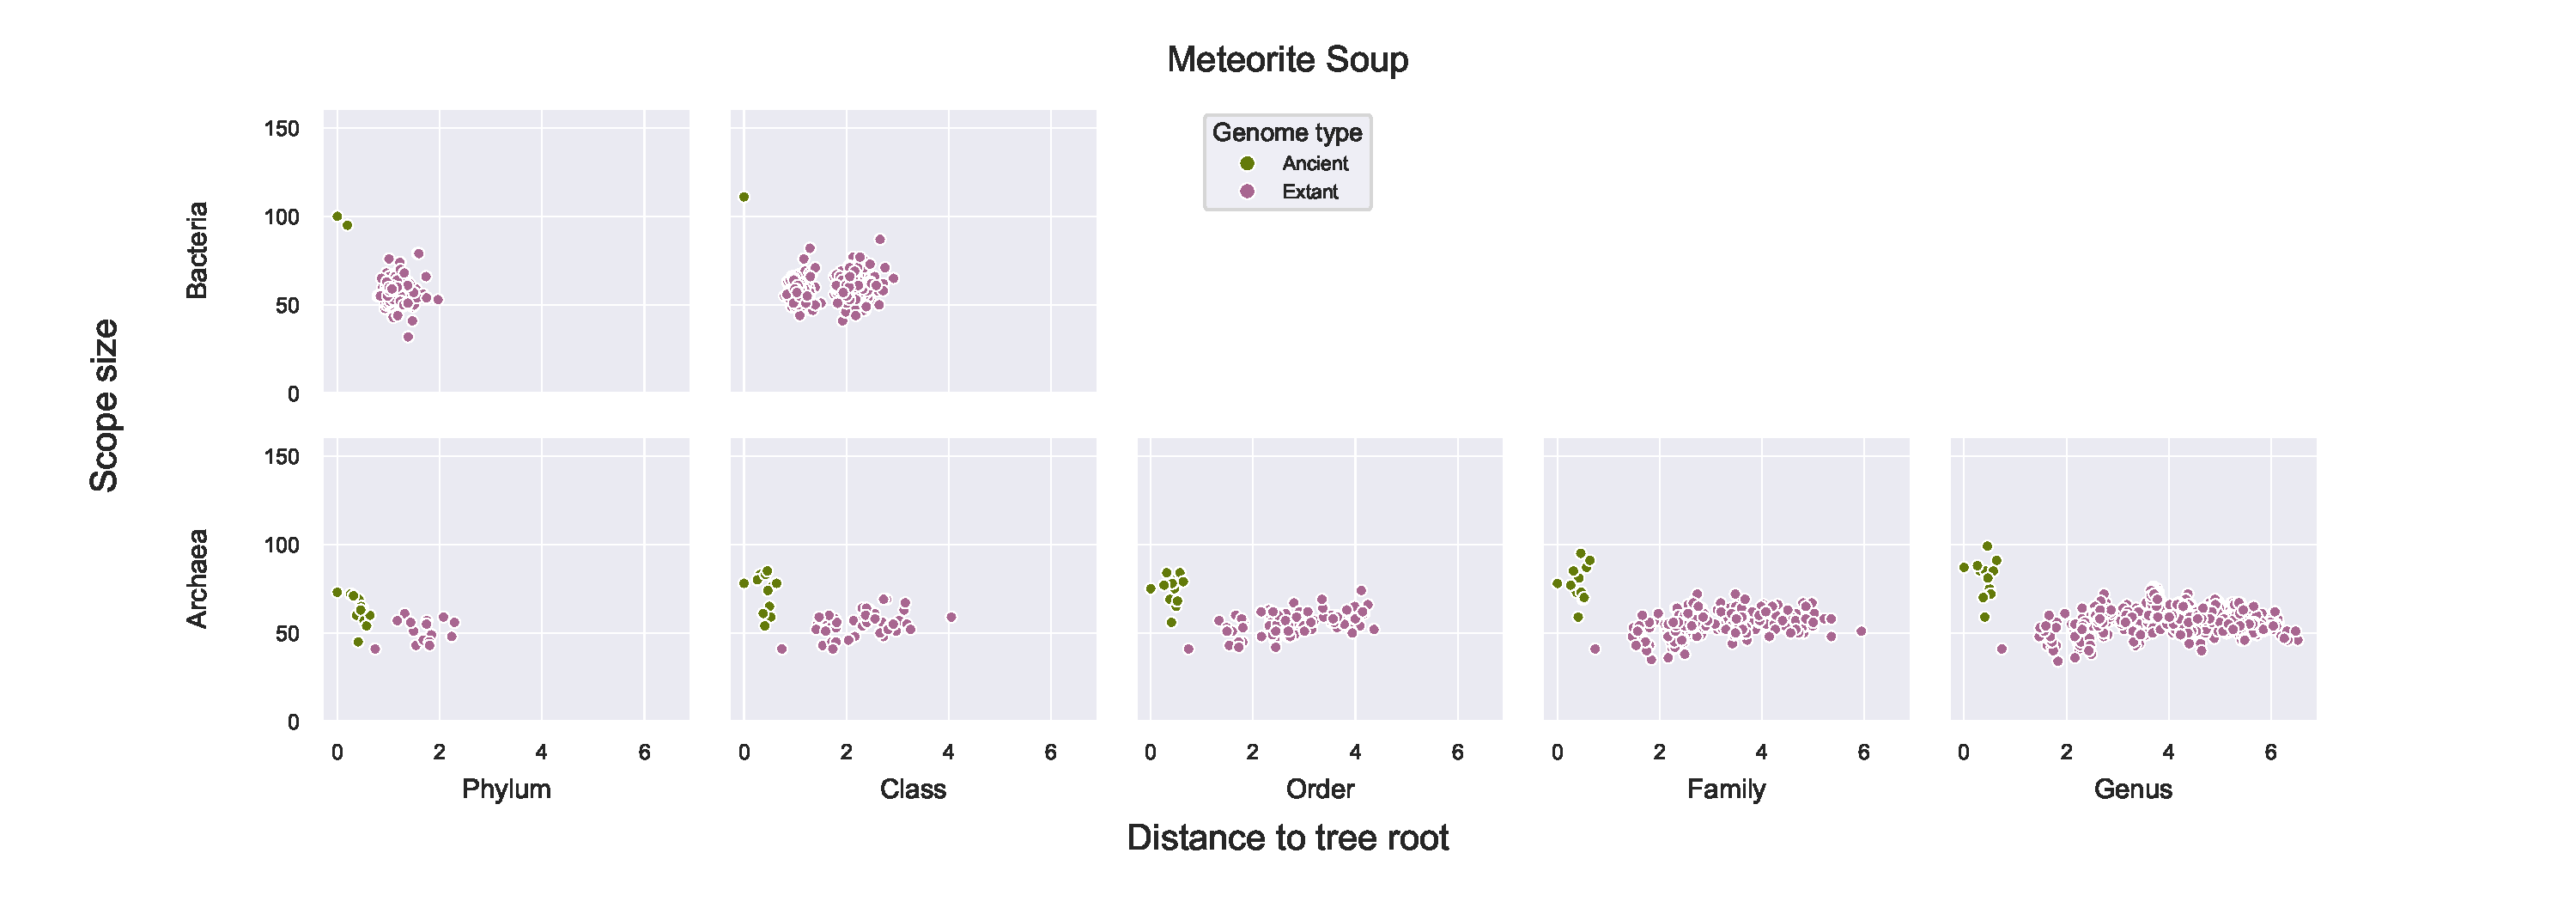
\includegraphics[width=0.95\textwidth]{scopesize_vs_disttoroot/gfm_ss_rootdist}
    \caption{Scope size as a function of distance to root for the meteorite soup seed set. In green: expansion on inferred ancient metabolic networks. In pink: expansion on extant metabolic networks. Each panel represents a different taxonomic level dataset.}
    \label{gfm_scopesize}
\end{figure}   

\begin{figure}[H]
    \centering
    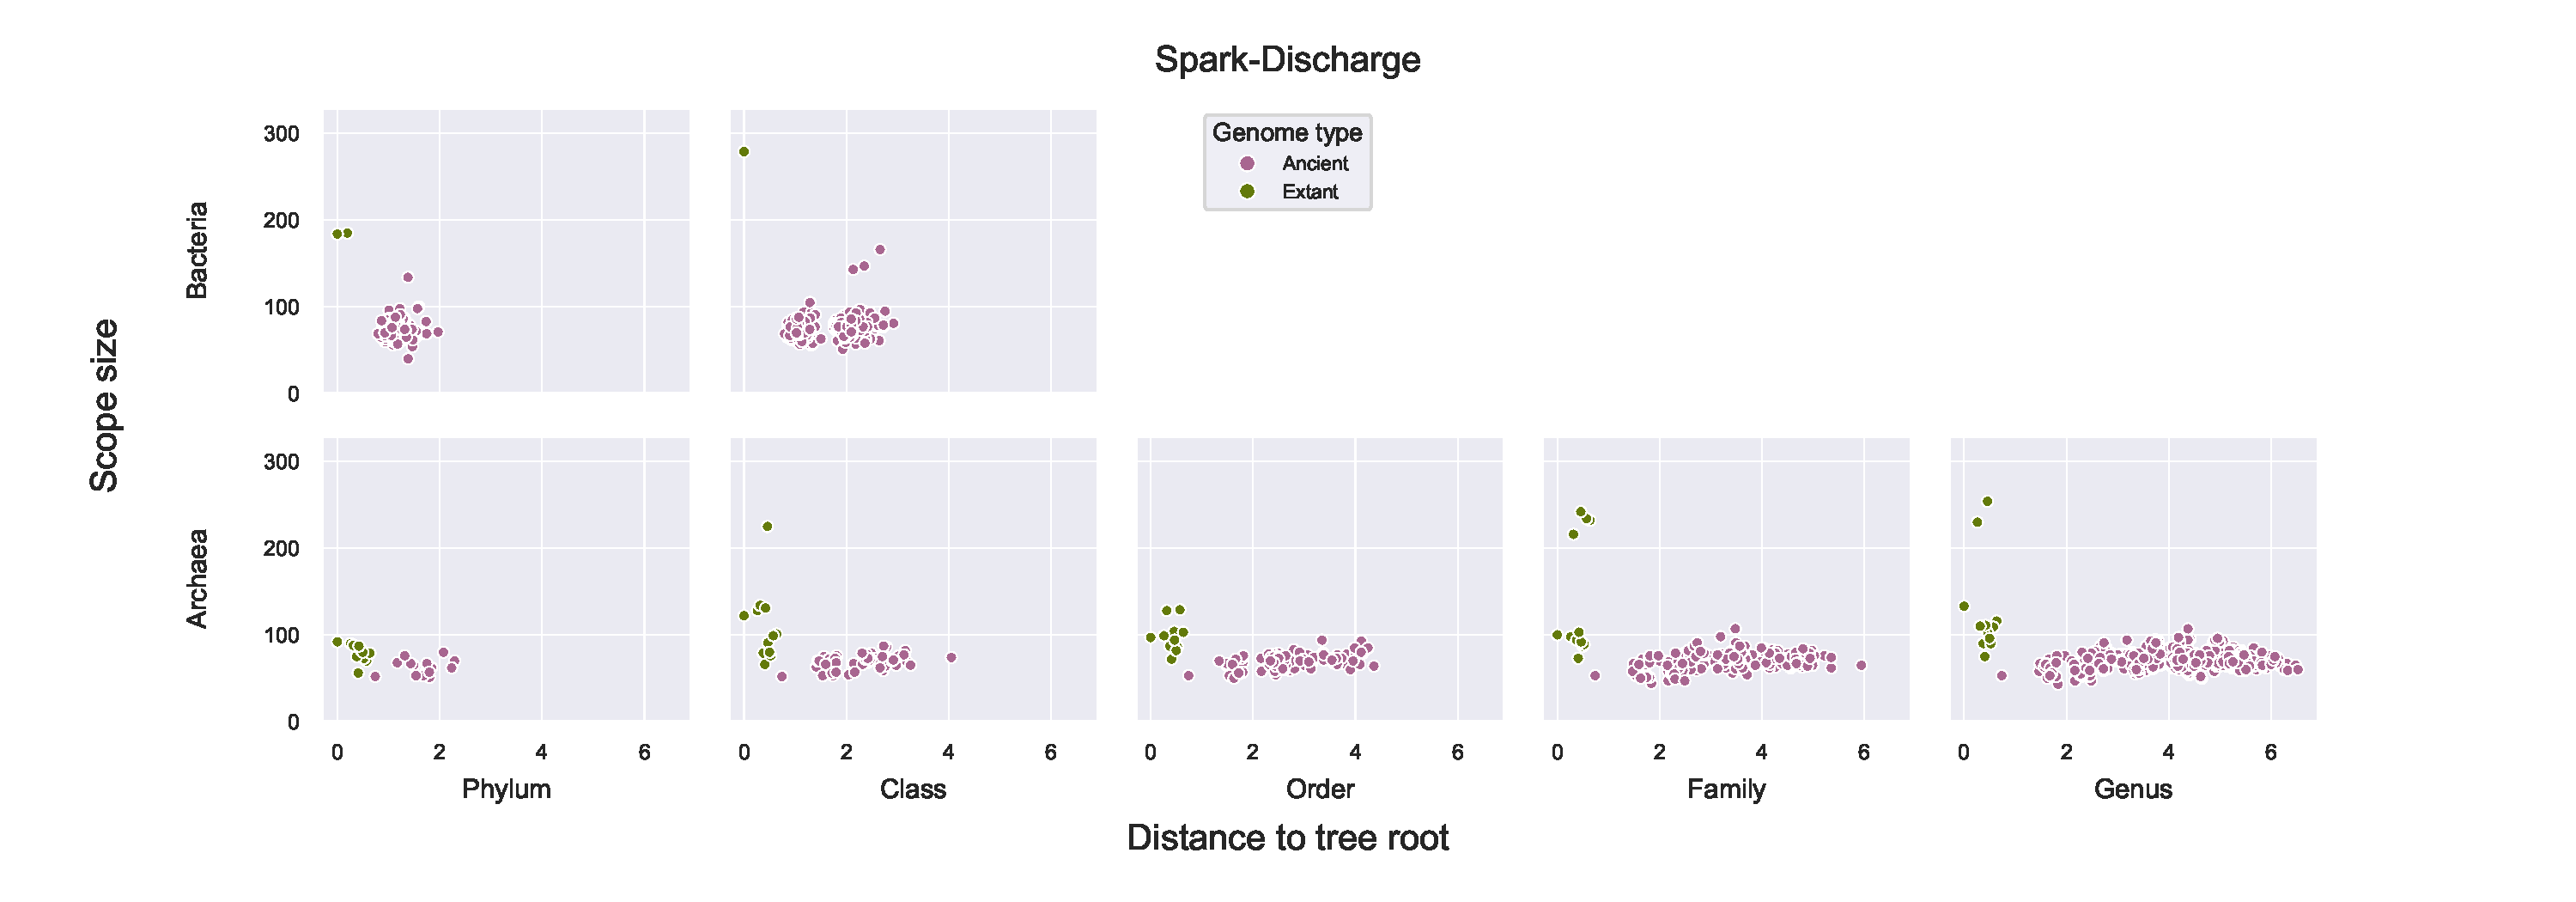
\includegraphics[width=0.95\textwidth]{scopesize_vs_disttoroot/gfsd_ss_rootdist.pdf}
    \caption{Scope size as a function of distance to root for the spark-discharge seed set. In green: expansion on inferred ancient metabolic networks. In pink: expansion on extant metabolic networks. Each panel represents a different taxonomic level dataset.}
    \label{gfsd_scopesize}
\end{figure}   

\begin{figure}[H]
    \centering
    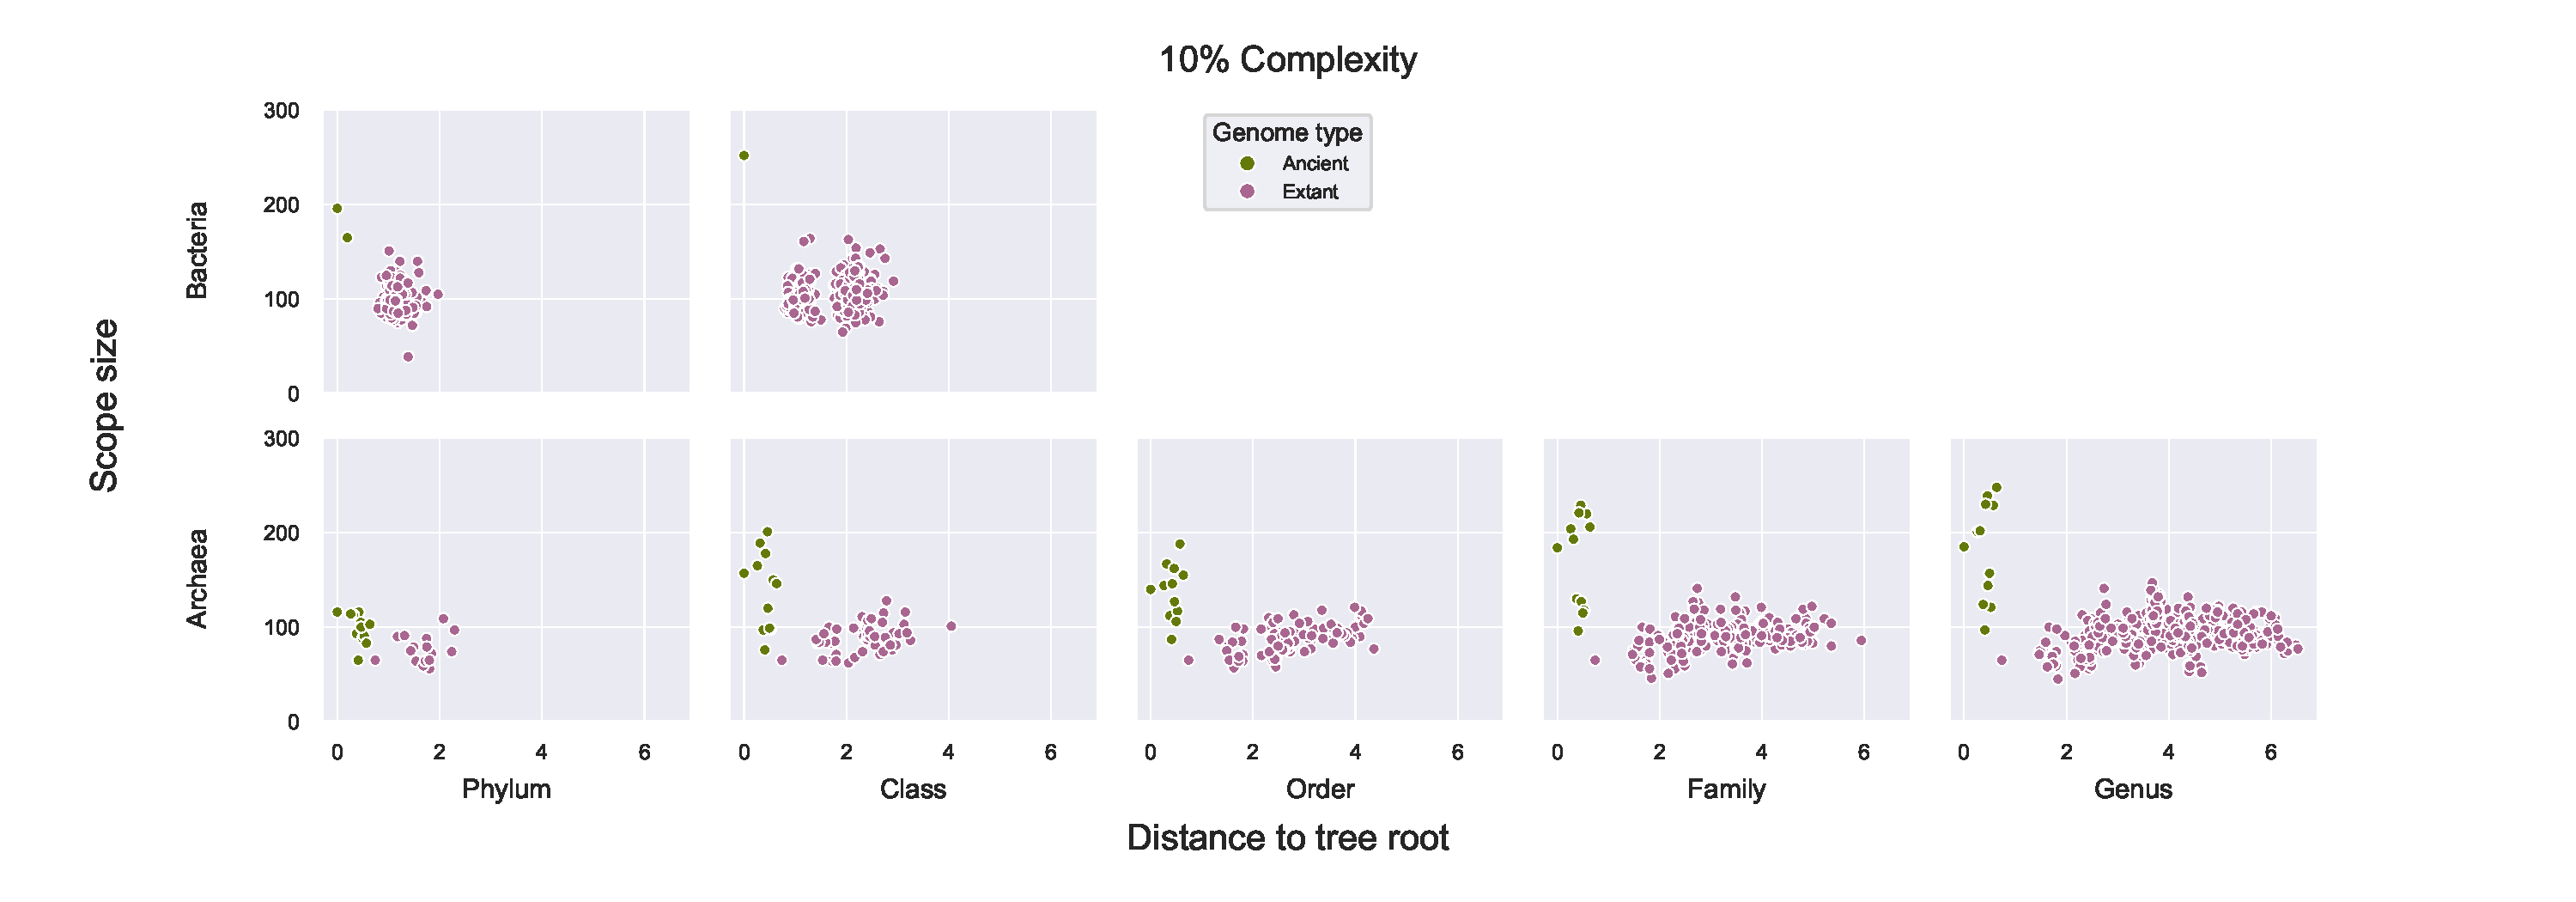
\includegraphics[width=0.95\textwidth]{scopesize_vs_disttoroot/0.1_ss_rootdist.pdf}
    \caption{Scope size as a function of distance to root for the 10\% complexity seed set. In green: expansion on inferred ancient metabolic networks. In pink: expansion on extant metabolic networks. Each panel represents a different taxonomic level dataset.}
    \label{0.1_scopesize}
\end{figure}   

\begin{figure}[H]
    \centering
    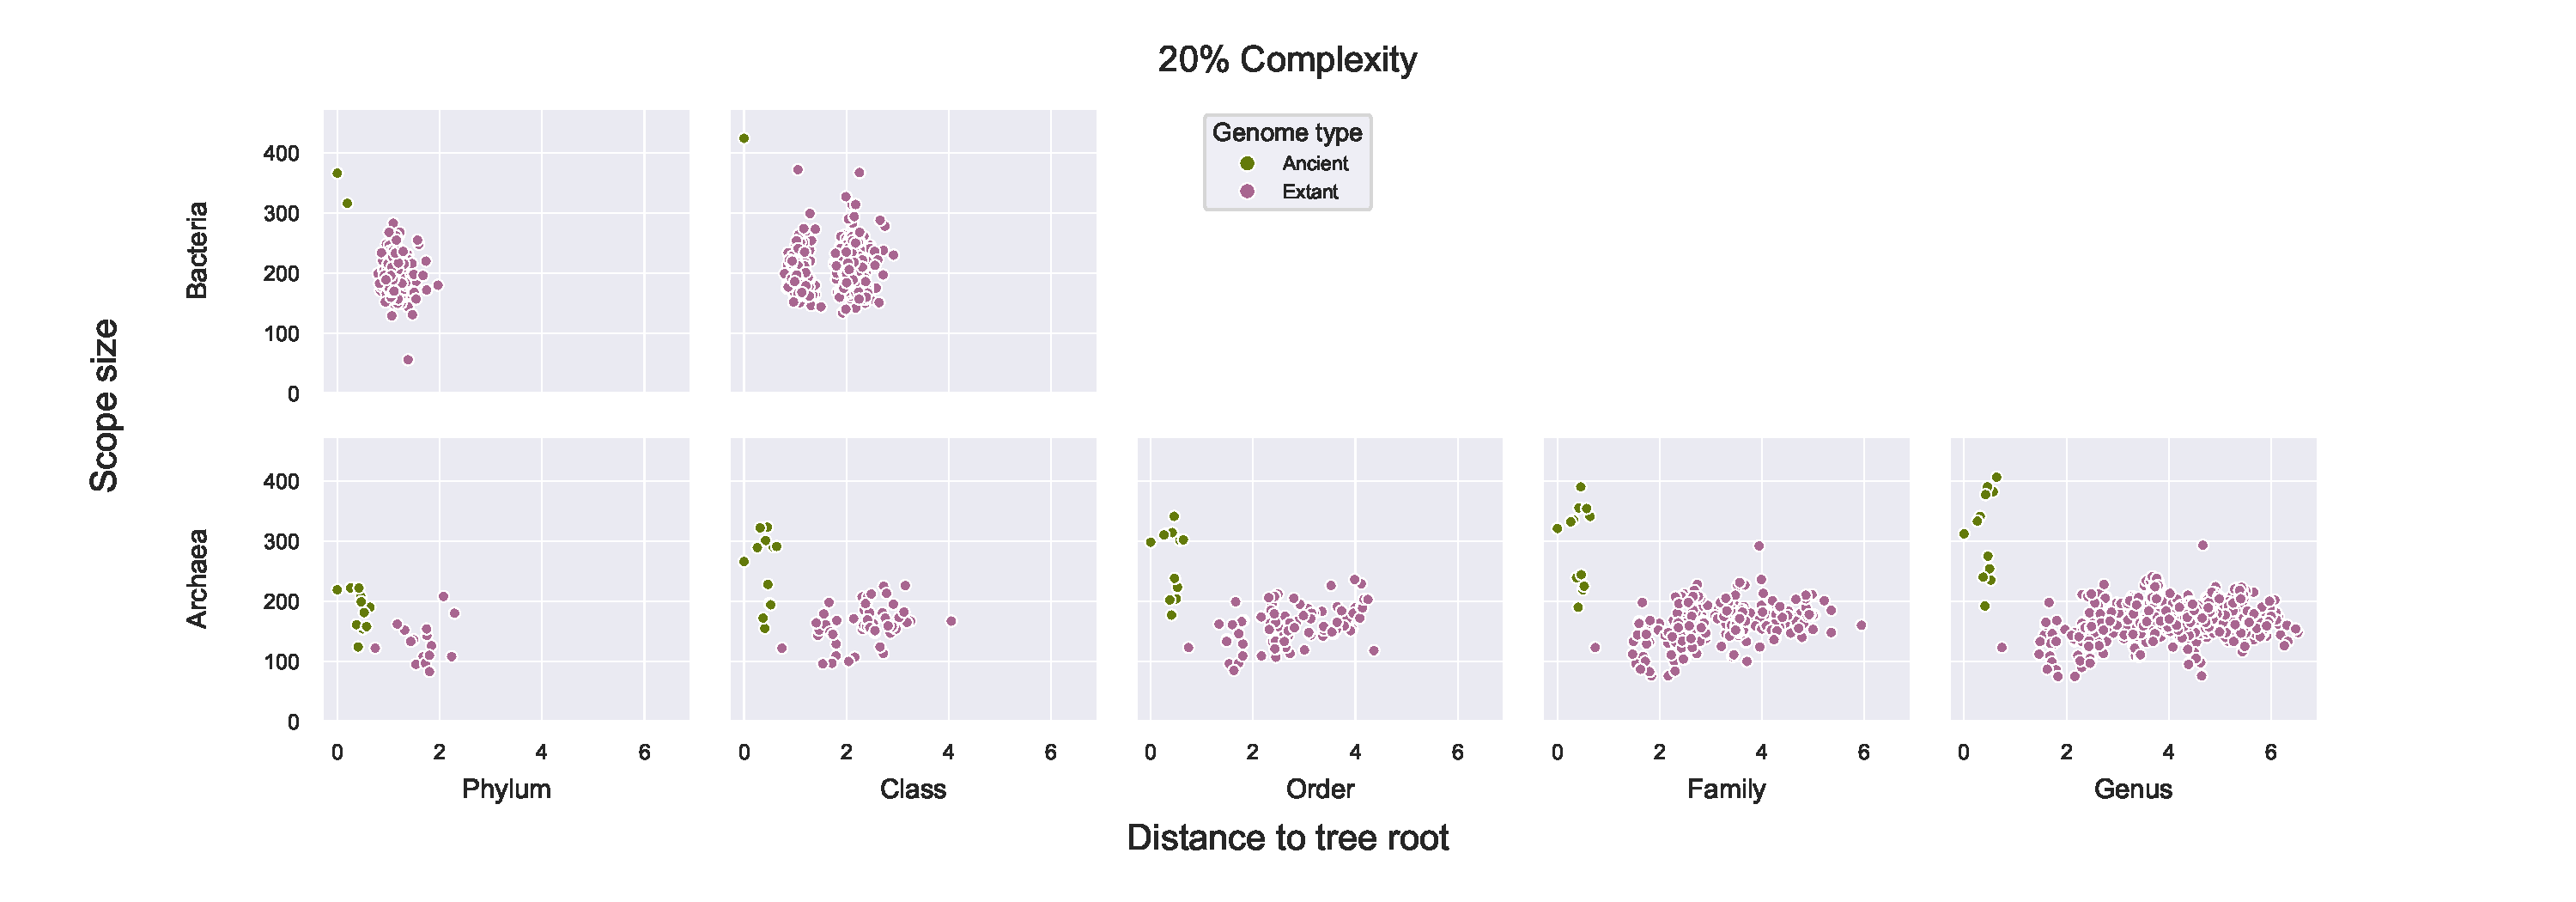
\includegraphics[width=0.95\textwidth]{scopesize_vs_disttoroot/0.2_ss_rootdist.pdf}
    \caption{Scope size as a function of distance to root for the 20\% complexity seed set. In green: expansion on inferred ancient metabolic networks. In pink: expansion on extant metabolic networks. Each panel represents a different taxonomic level dataset.}
    \label{0.2_scopesize}
\end{figure}   

\begin{figure}[H]
    \centering
    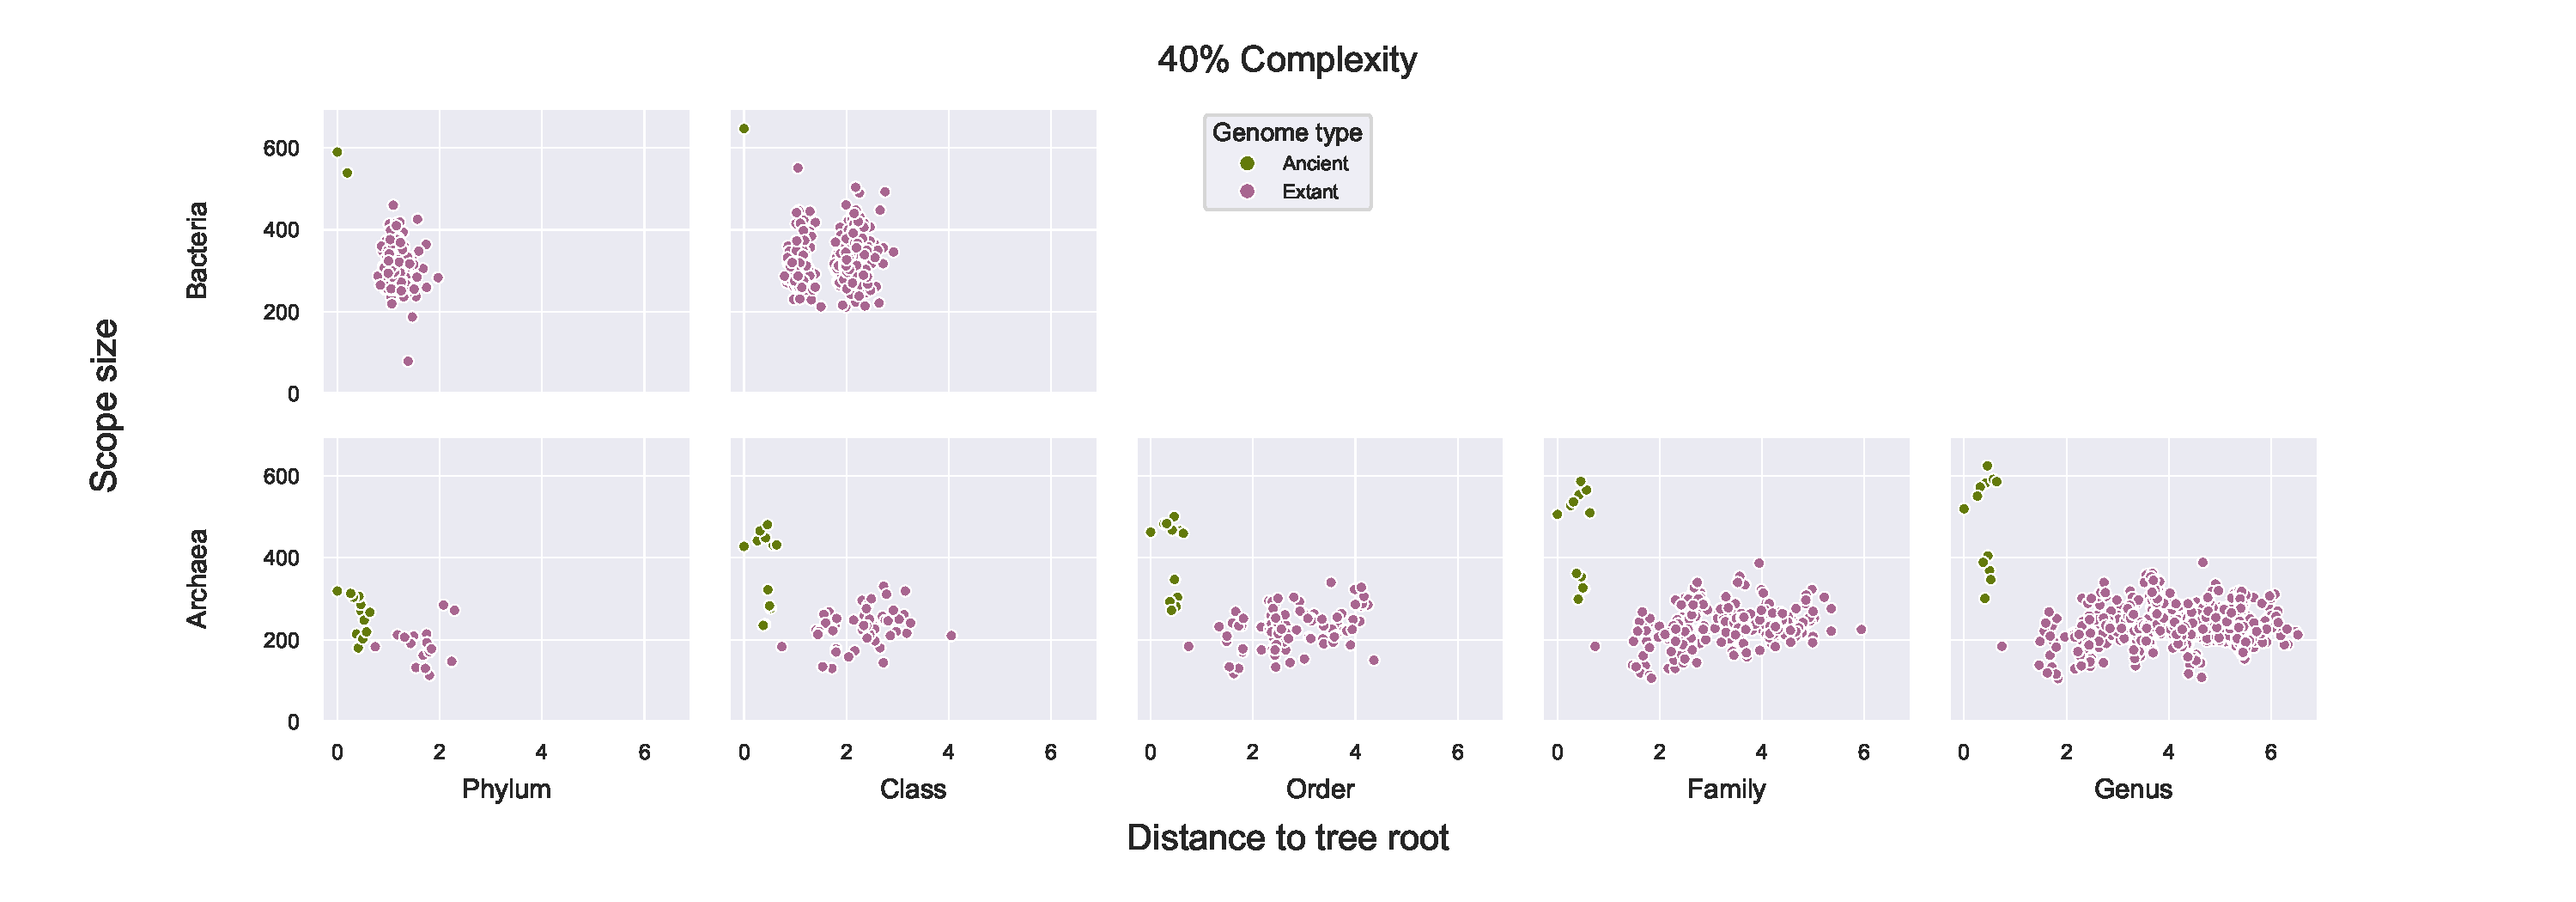
\includegraphics[width=0.95\textwidth]{scopesize_vs_disttoroot/0.4_ss_rootdist.pdf}
    \caption{Scope size as a function of distance to root for the 40\% complexity seed set. In green: expansion on inferred ancient metabolic networks. In pink: expansion on extant metabolic networks. Each panel represents a different taxonomic level dataset.}
    \label{0.4_scopesize}
\end{figure}   

\begin{figure}[H]
    \centering
    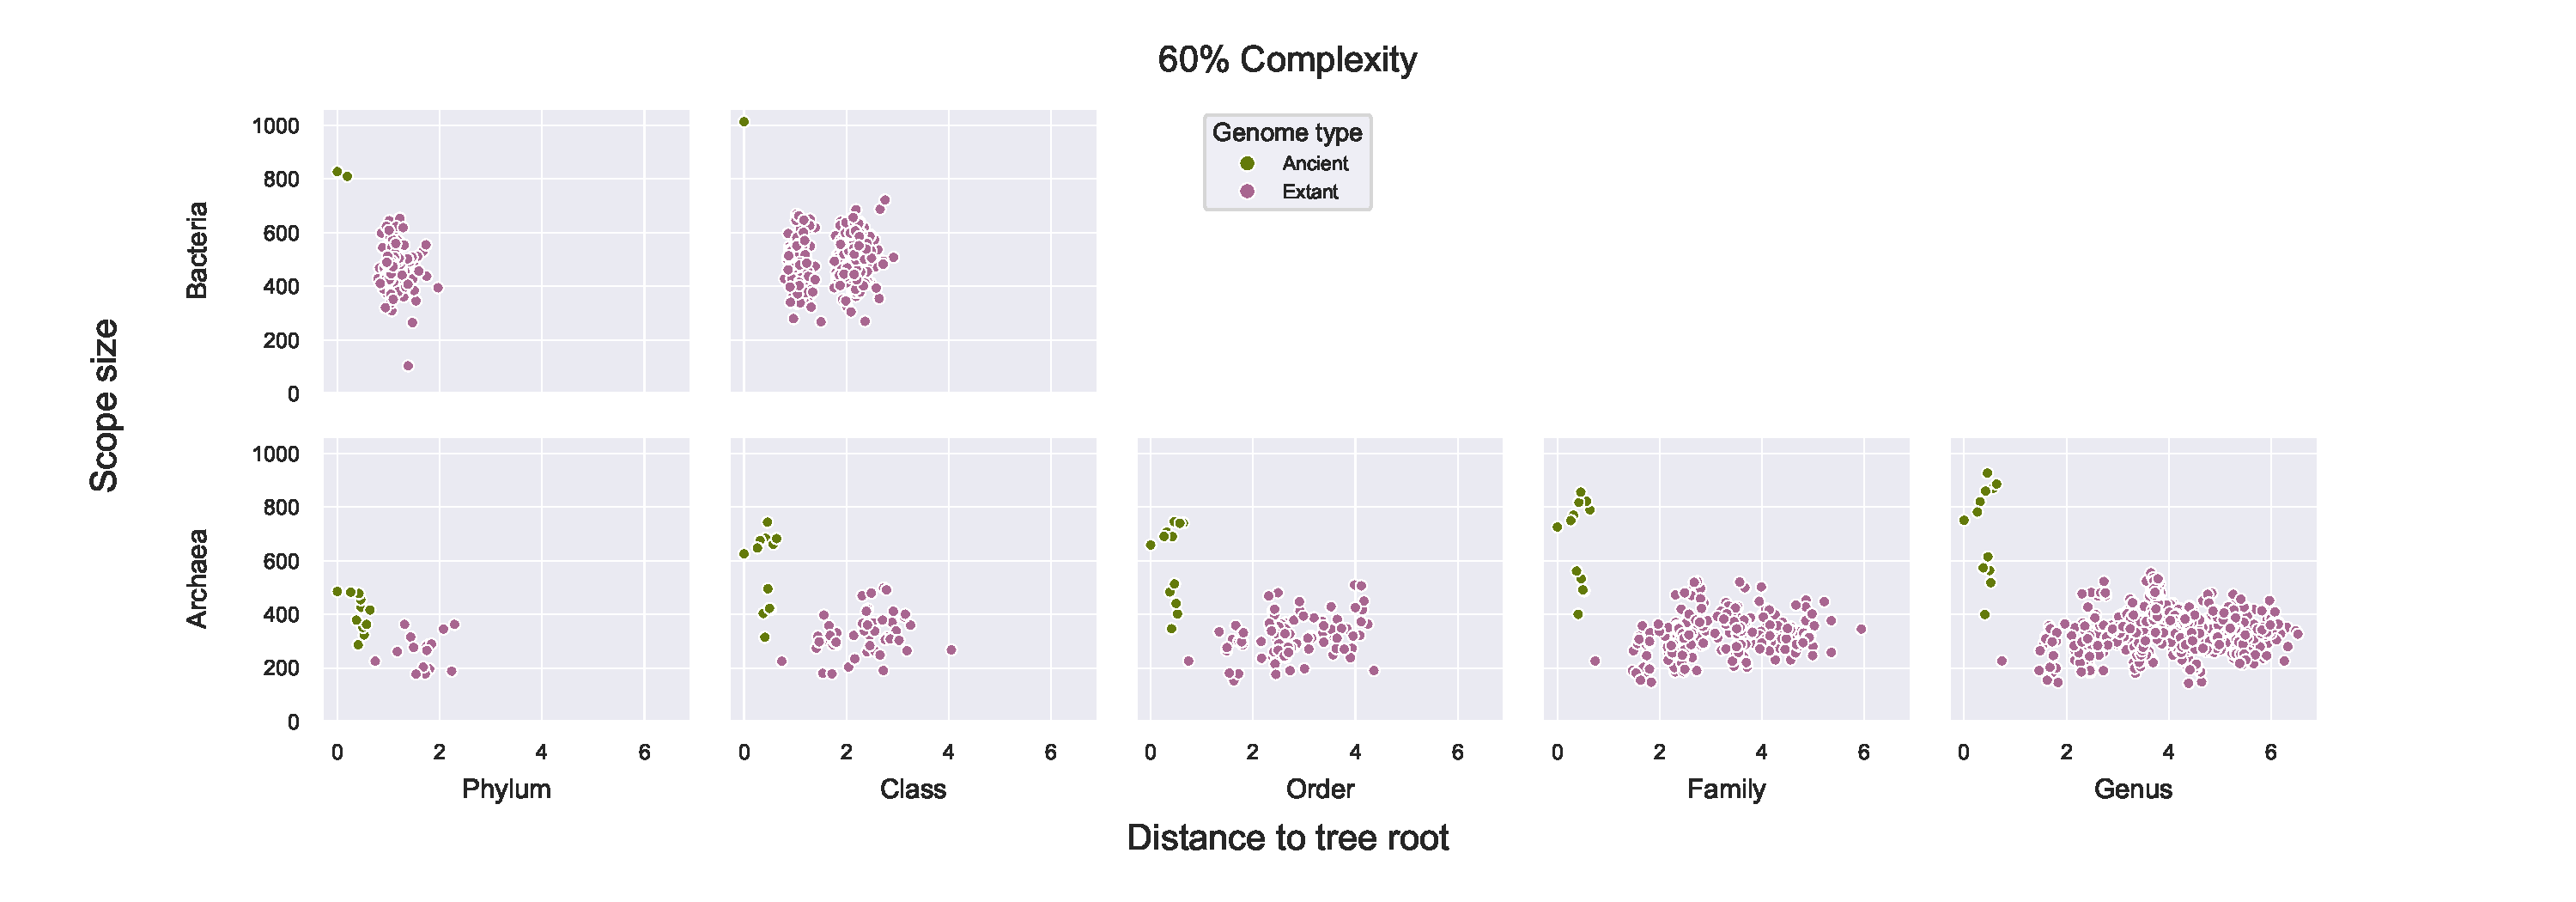
\includegraphics[width=0.95\textwidth]{scopesize_vs_disttoroot/0.6_ss_rootdist.pdf}
    \caption{Scope size as a function of distance to root for the 60\% complexity seed set. In green: expansion on inferred ancient metabolic networks. In pink: expansion on extant metabolic networks. Each panel represents a different taxonomic level dataset.}
    \label{0.6_scopesize}
\end{figure}   

\begin{figure}[H]
    \centering
    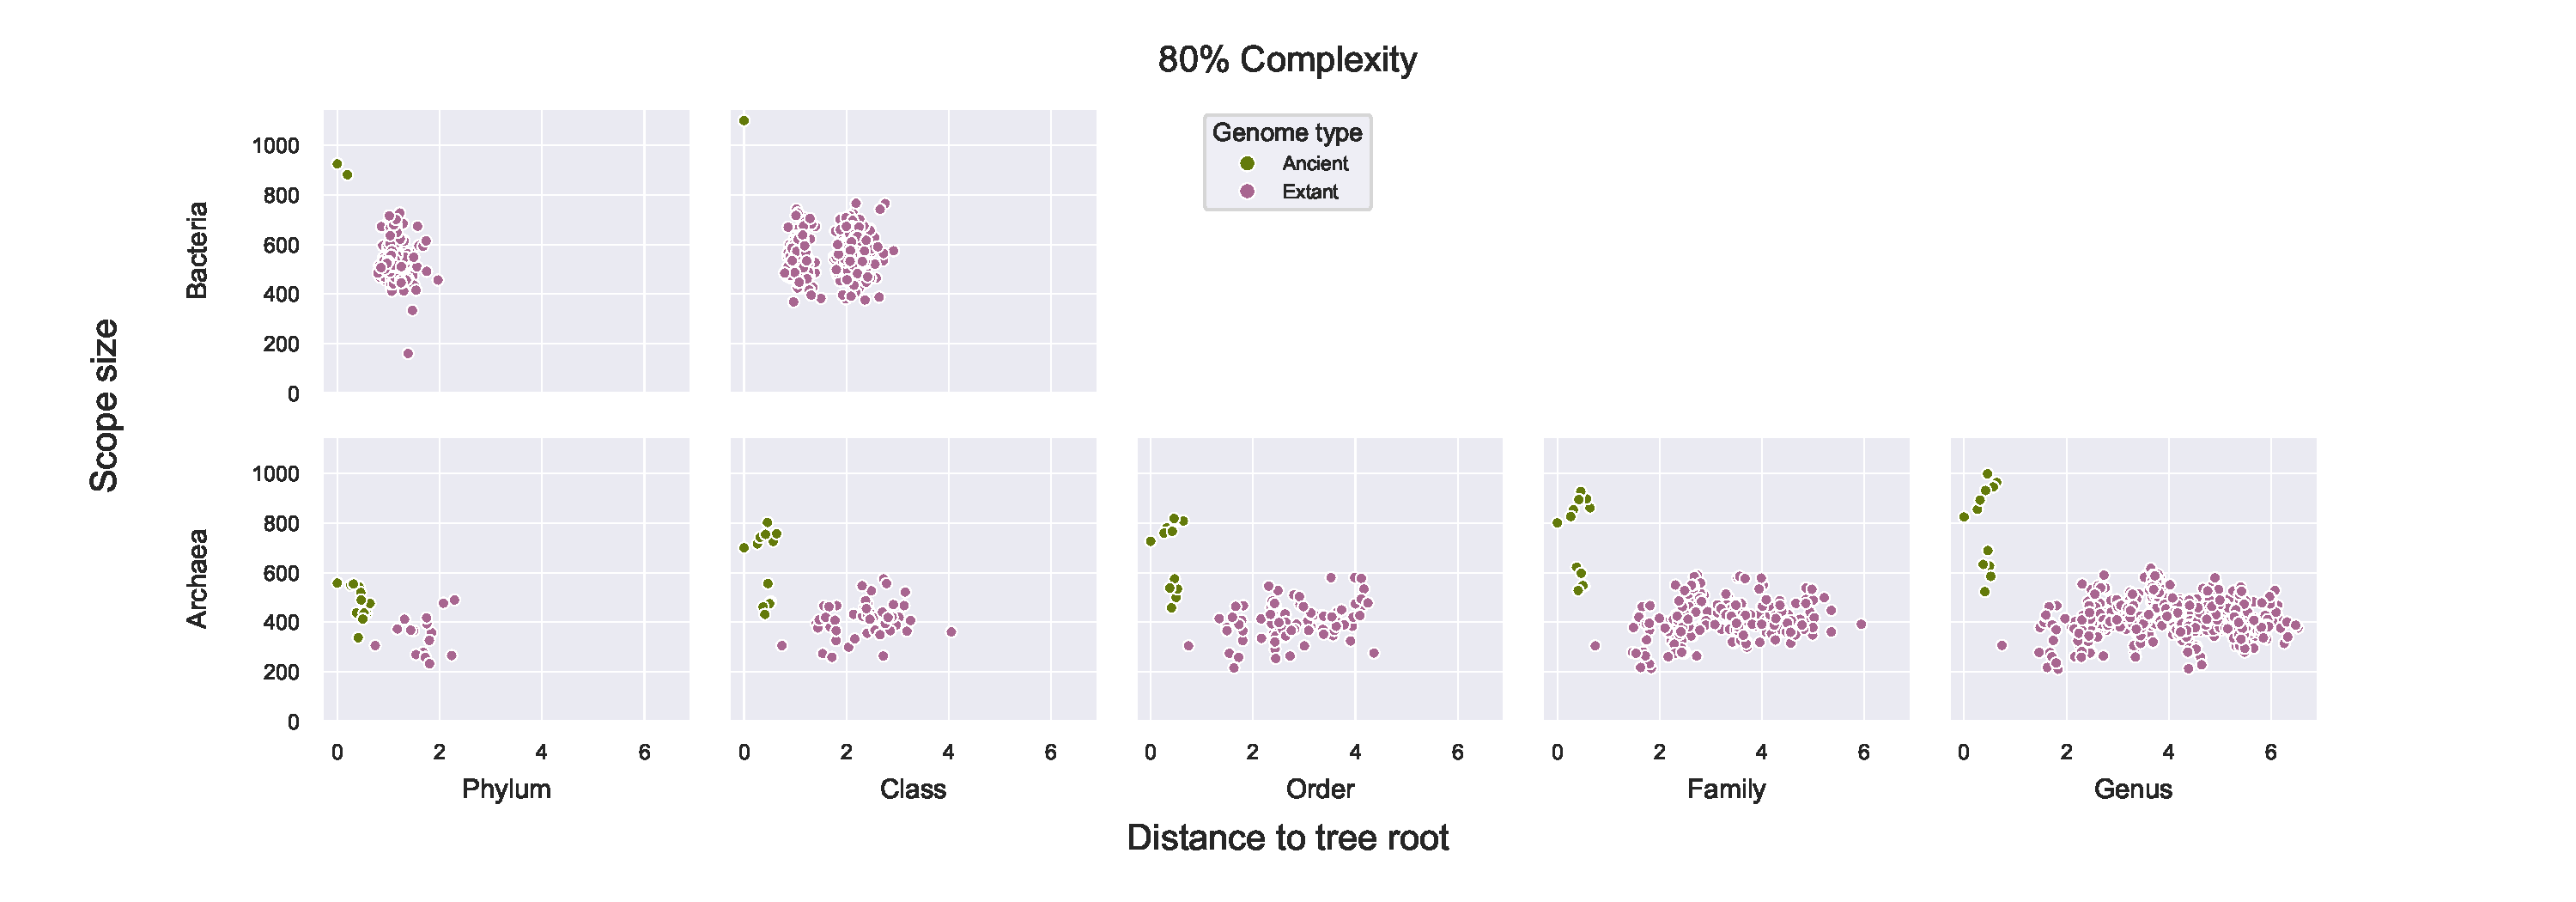
\includegraphics[width=0.95\textwidth]{scopesize_vs_disttoroot/0.8_ss_rootdist.pdf}
    \caption{Scope size as a function of distance to root for the 80\% complexity seed set. In green: expansion on inferred ancient metabolic networks. In pink: expansion on extant metabolic networks. Each panel represents a different taxonomic level dataset.}
    \label{0.8_scopesize}
\end{figure}   

\begin{figure}[H]
    \centering
    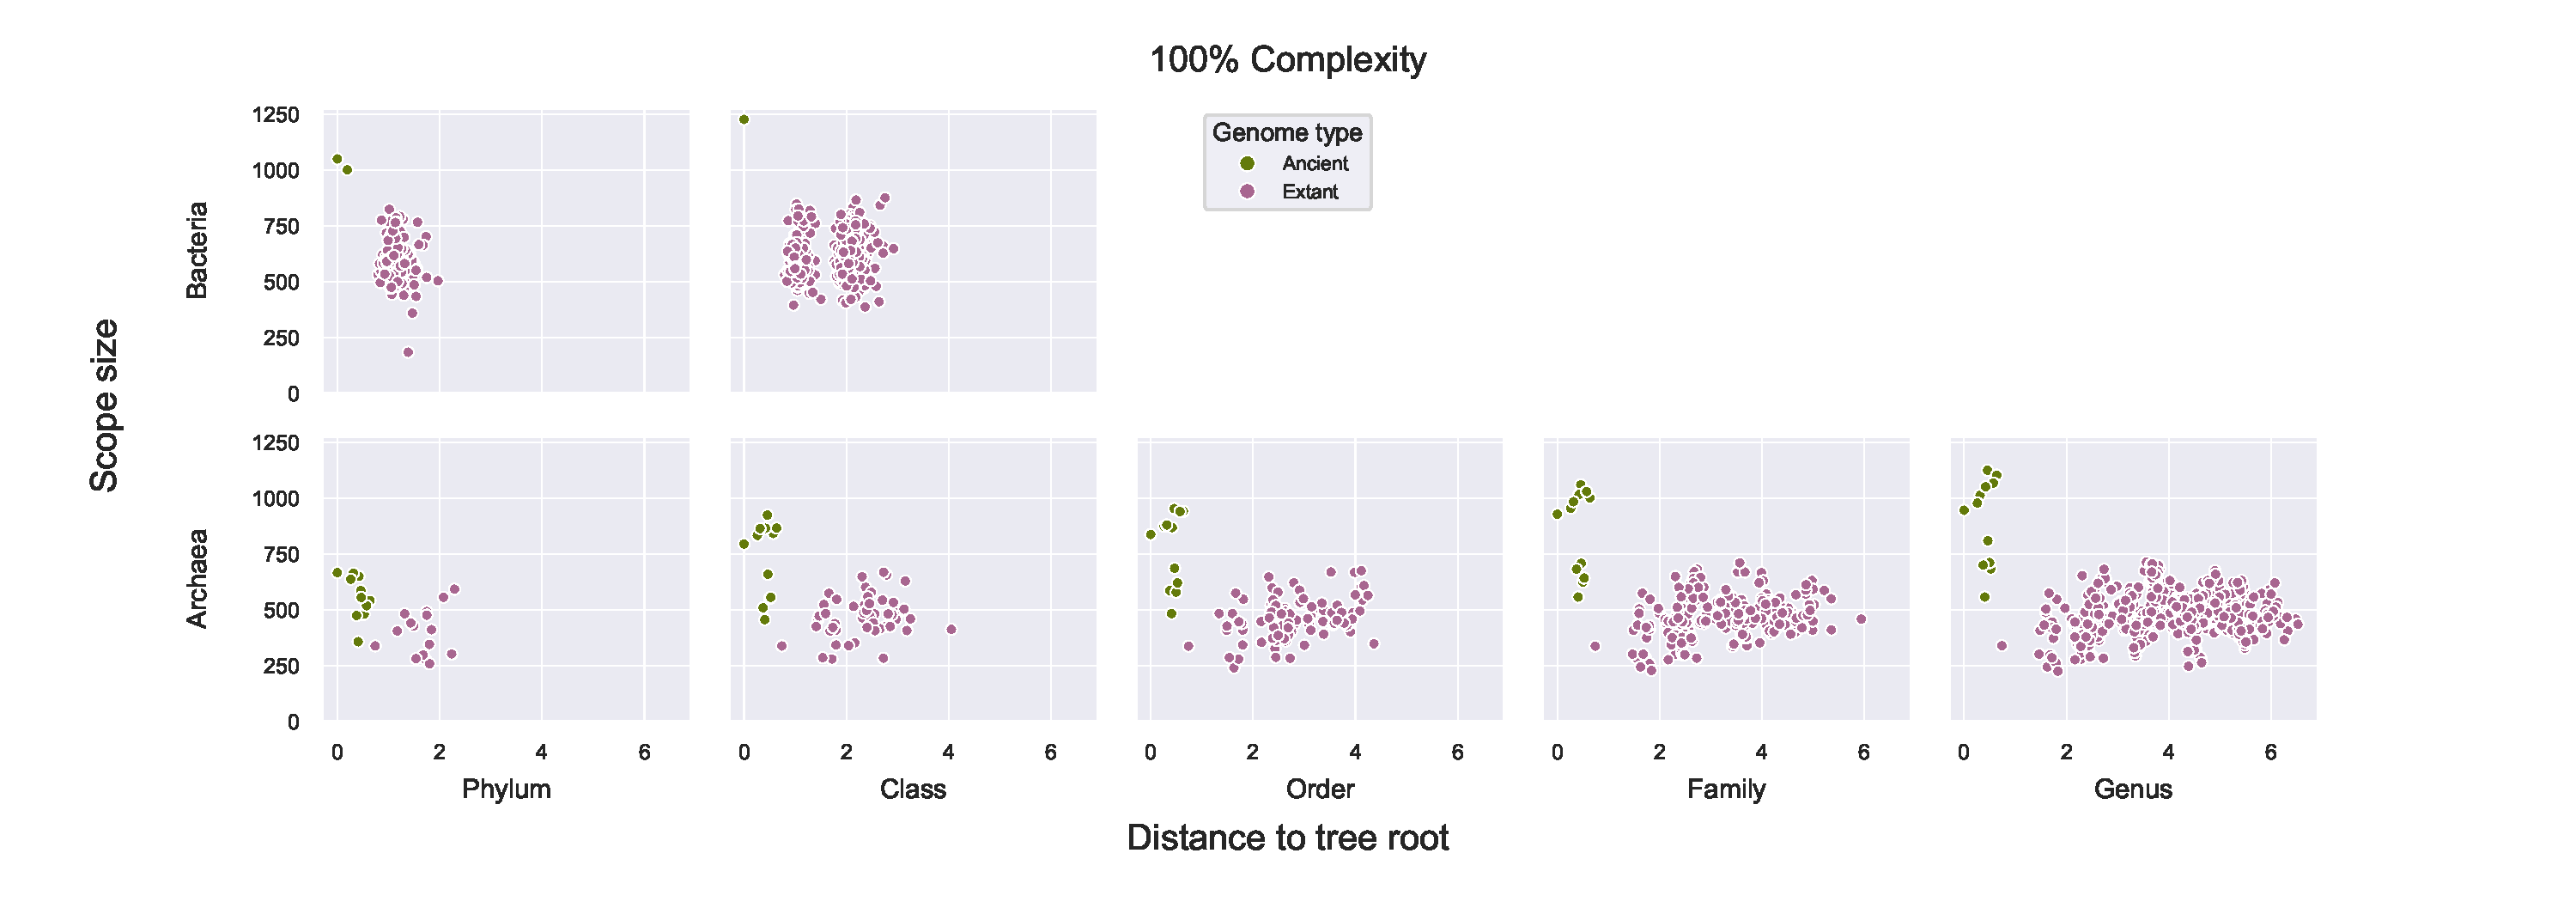
\includegraphics[width=0.95\textwidth]{scopesize_vs_disttoroot/1_ss_rootdist.pdf}
    \caption{Scope size as a function of distance to root for the 100\% complexity seed set. In green: expansion on inferred ancient metabolic networks. In pink: expansion on extant metabolic networks. Each panel represents a different taxonomic level dataset.}
    \label{1_scopesize}
\end{figure}   

% \textbf{For every seed set, per taxonomic level dataset.}

% \begin{figure}[H]
%     \centering
%     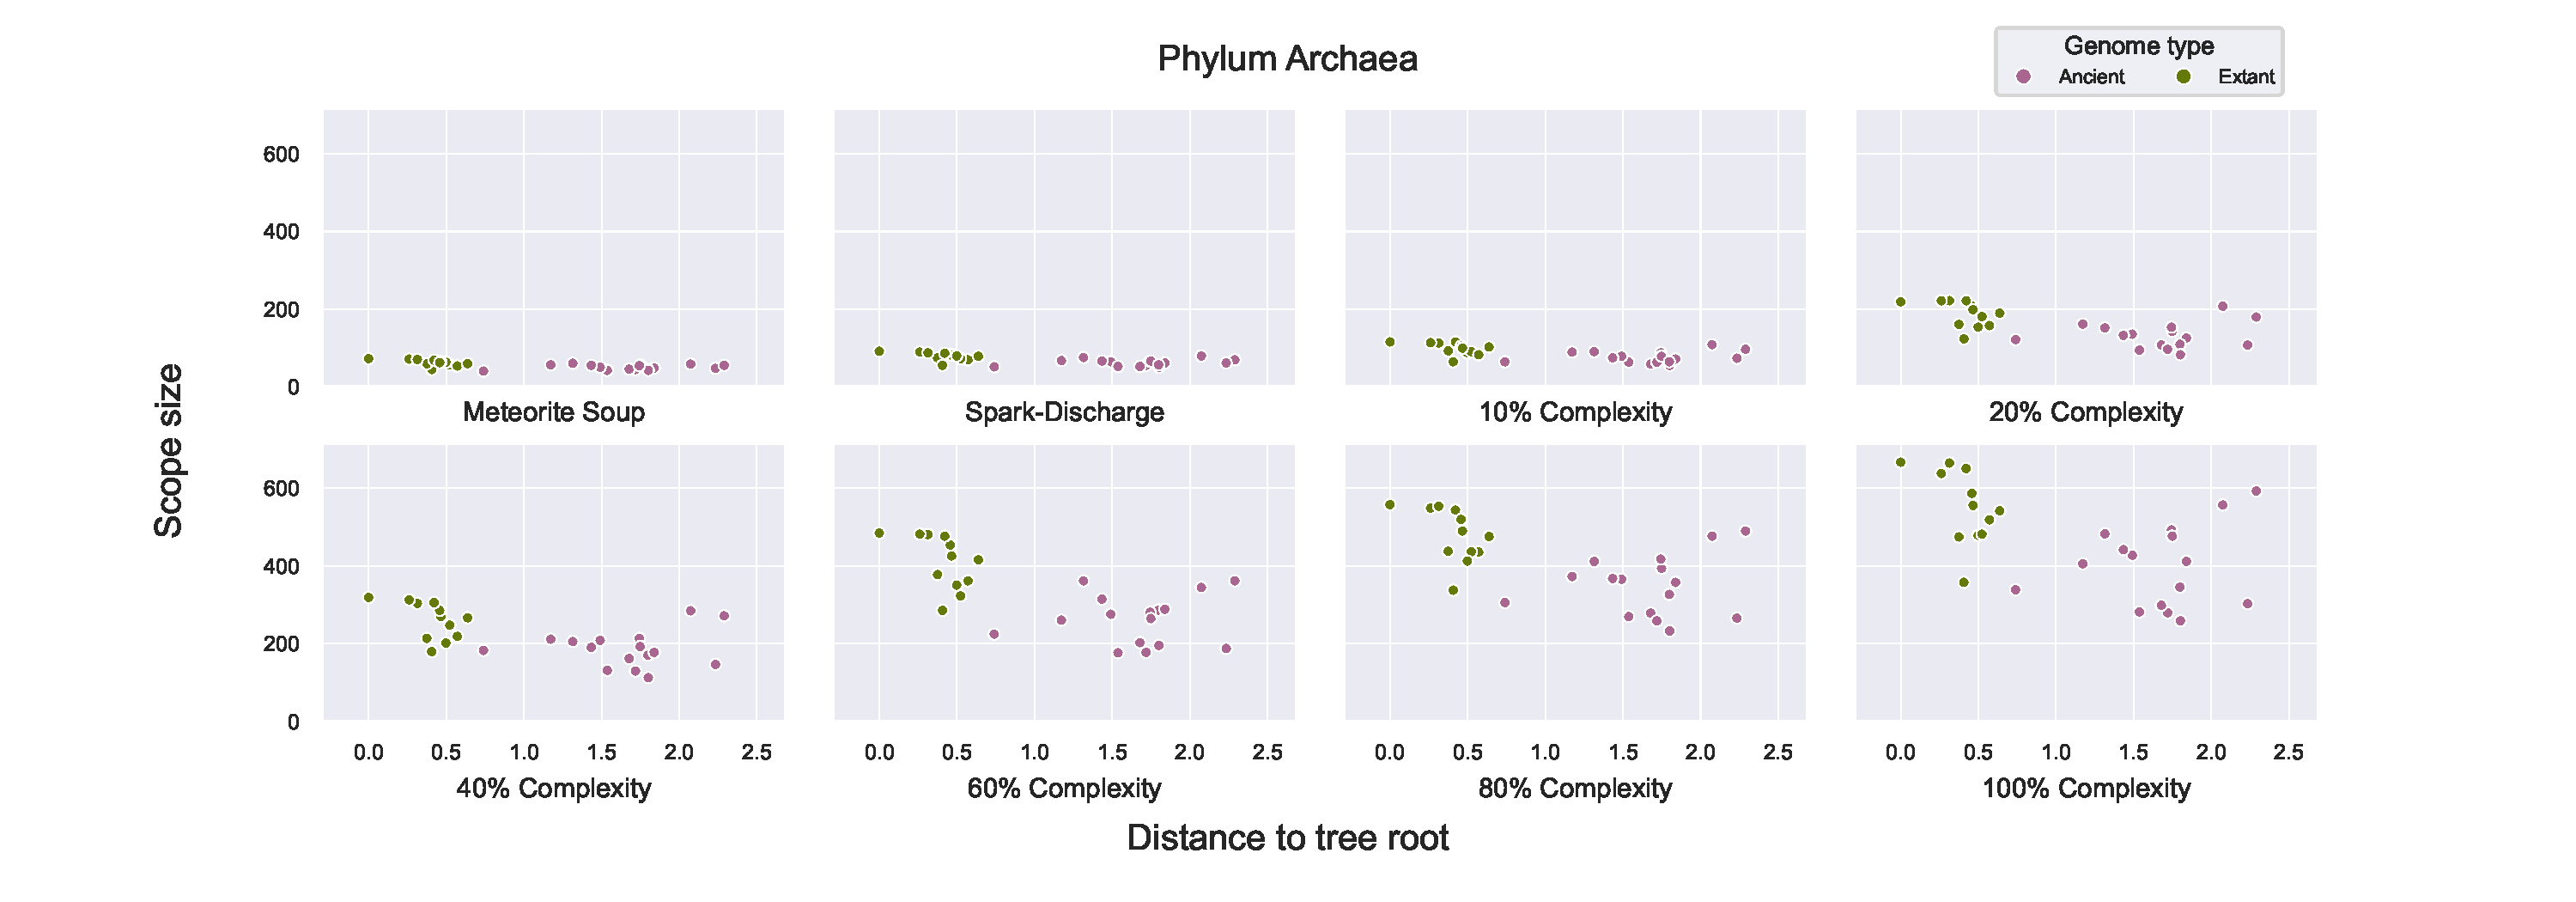
\includegraphics[width=0.95\textwidth]{scopesize_vs_disttoroot/phy4arc_ss_rootdist.pdf}
%     \caption{Phylum level archaea}
%     \label{phyarc_scopesize}
% \end{figure}   

% \begin{figure}[H]
%     \centering
%     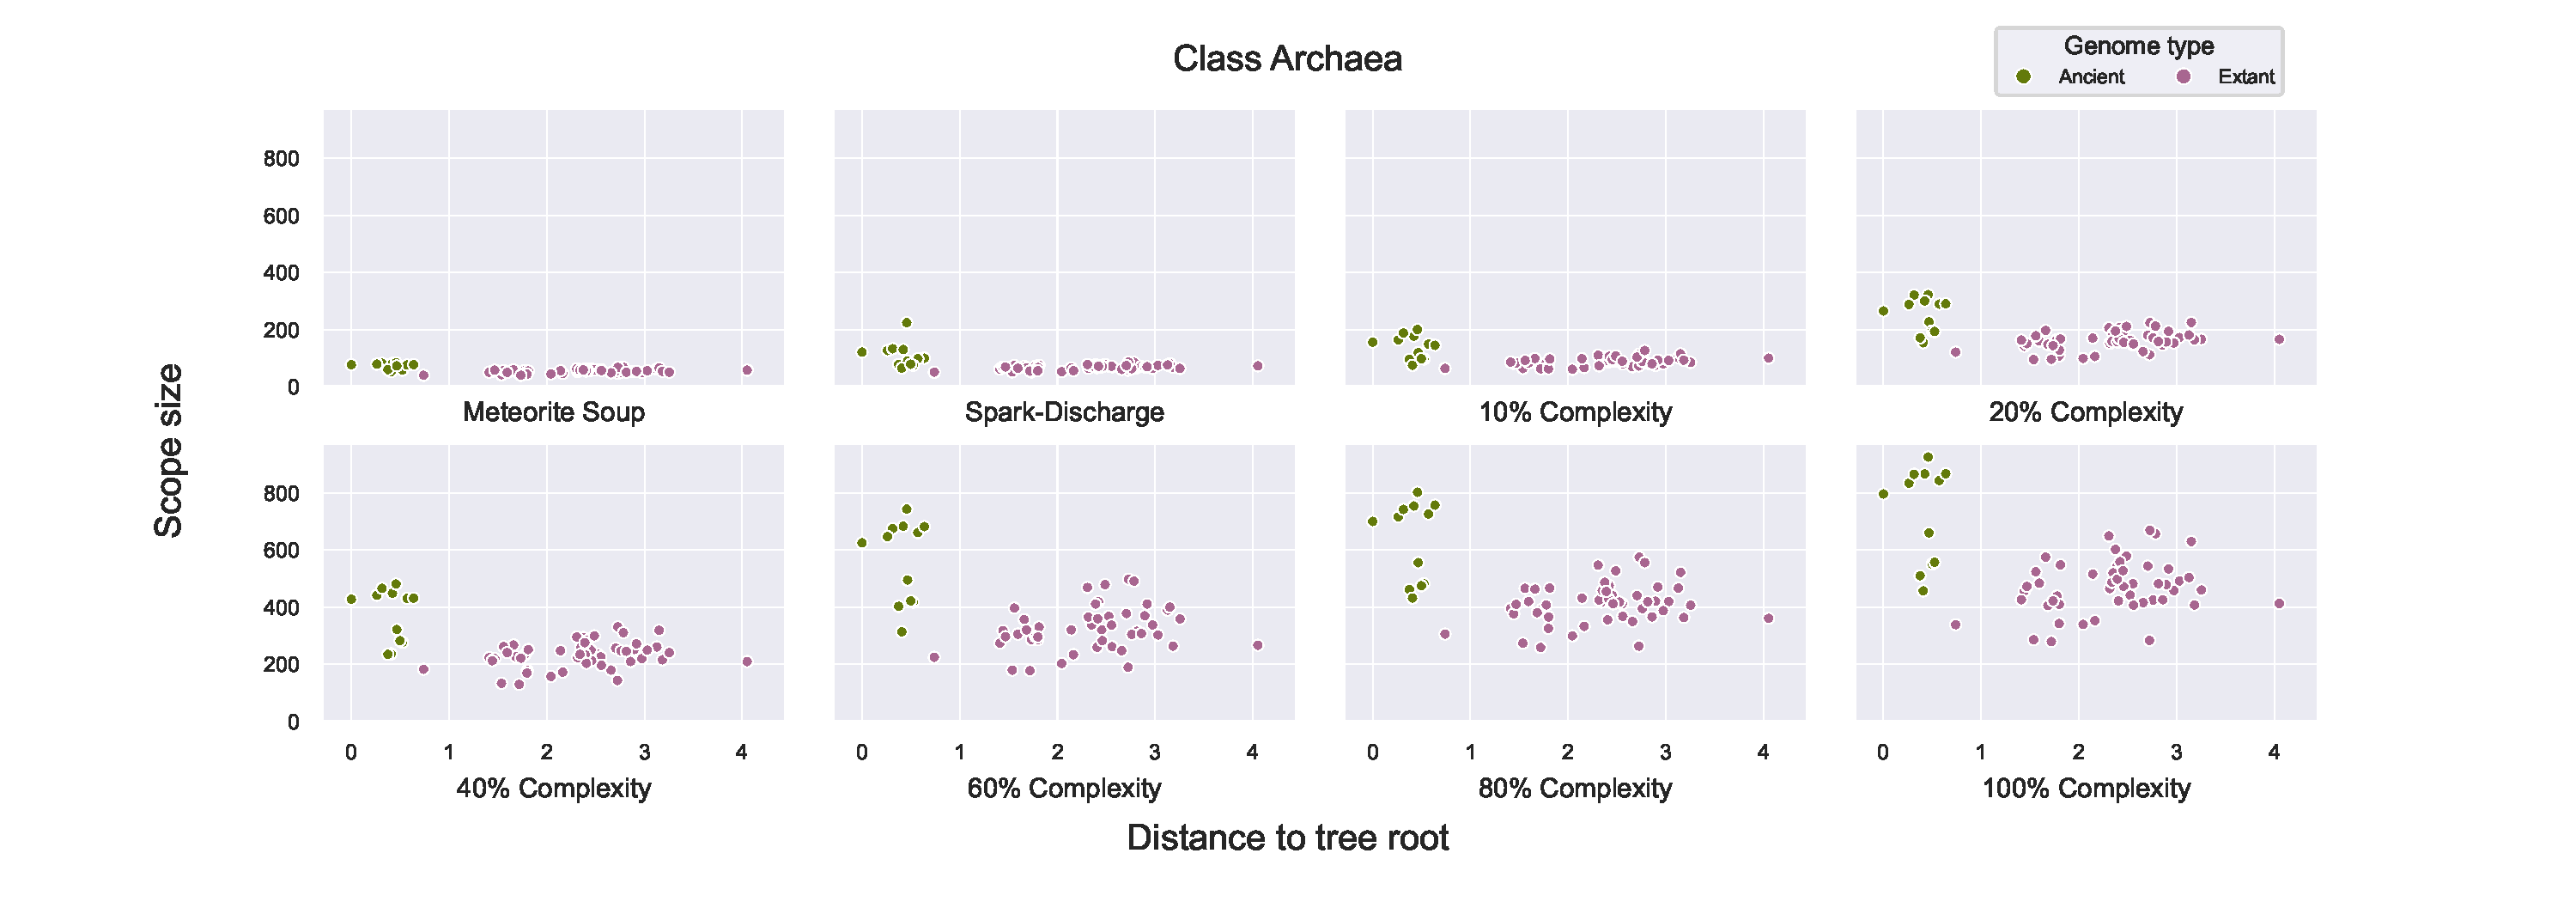
\includegraphics[width=0.95\textwidth]{scopesize_vs_disttoroot/cla4arc_ss_rootdist.pdf}
%     \caption{Class level archaea}
%     \label{claarc_scopesize}
% \end{figure}   

% \begin{figure}[H]
%     \centering
%     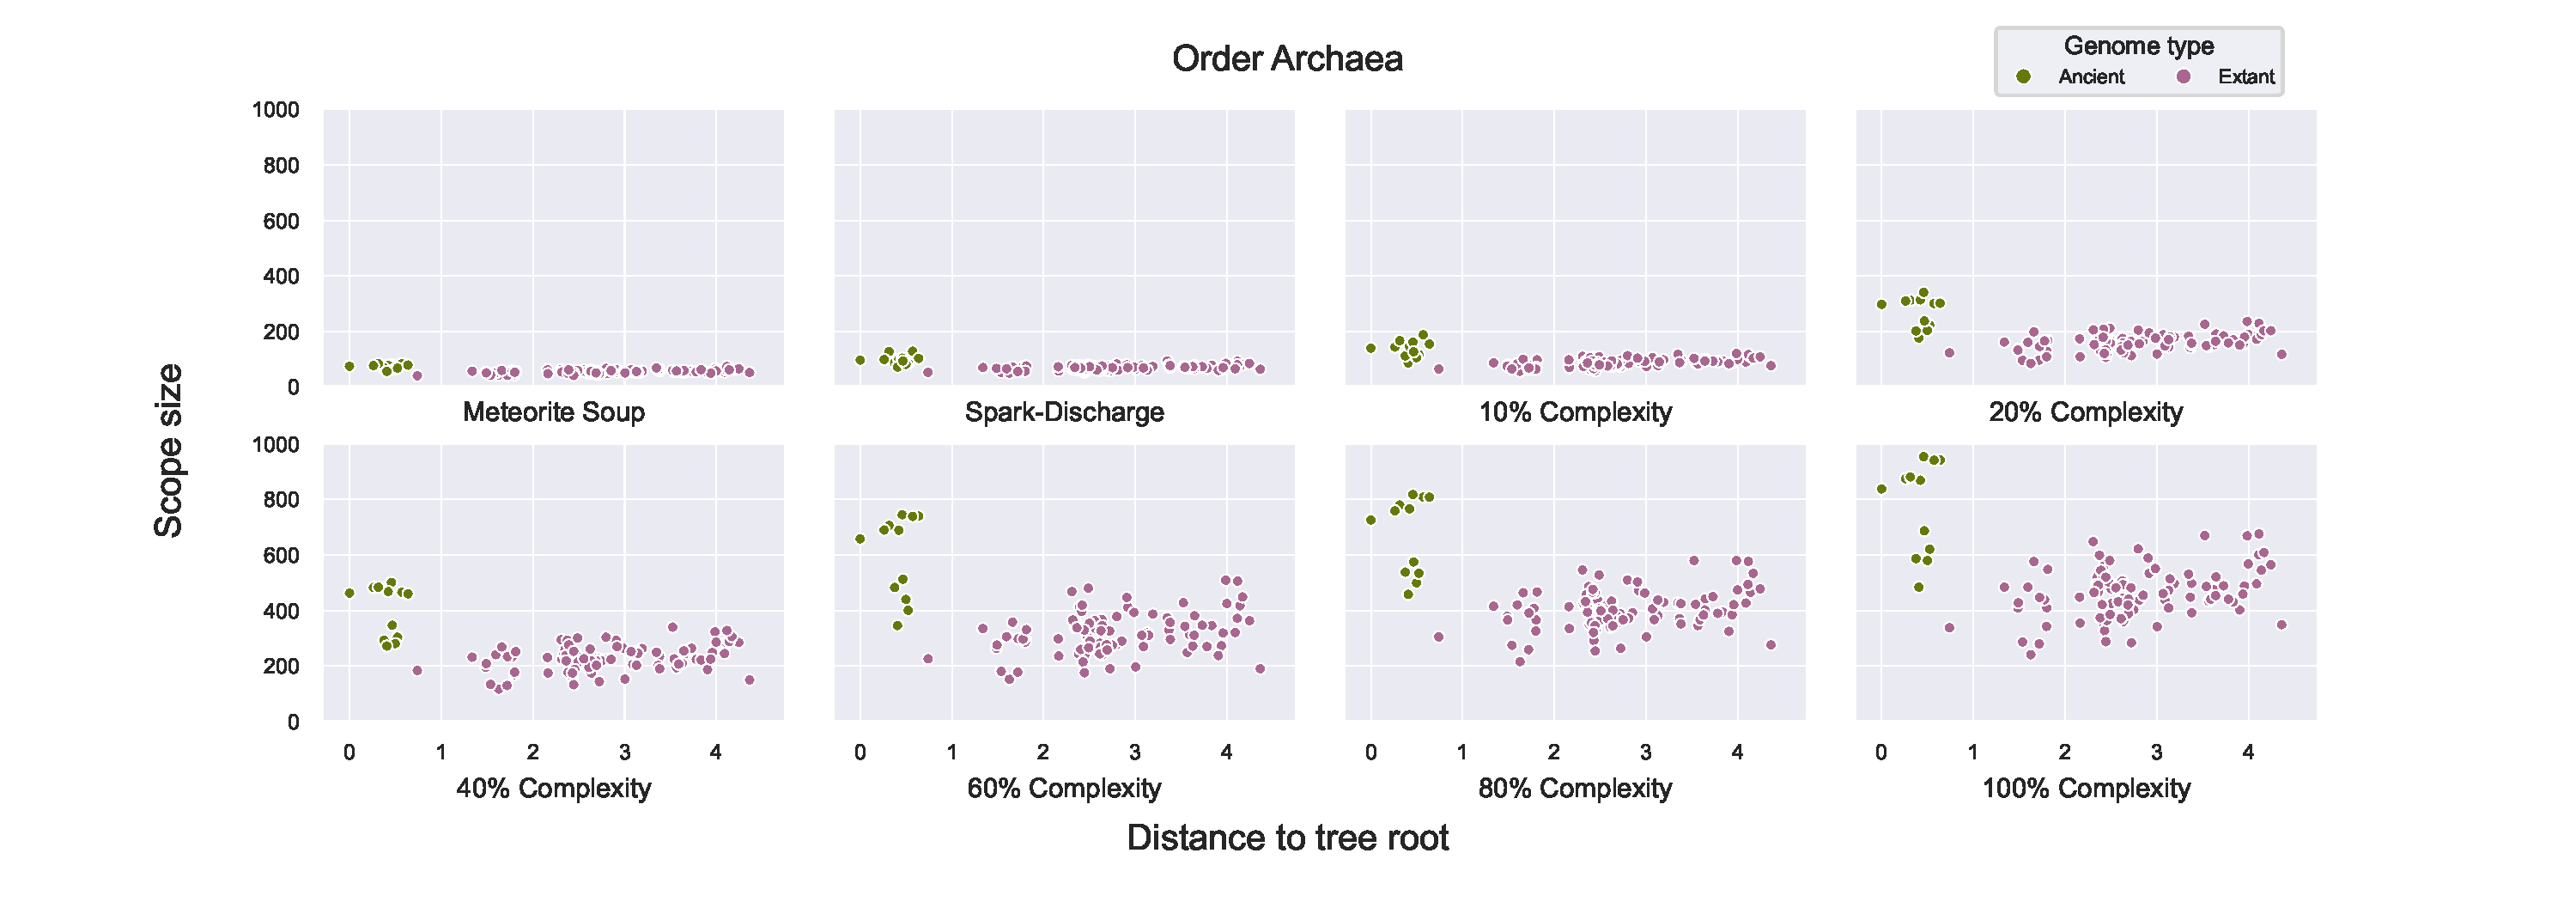
\includegraphics[width=0.95\textwidth]{scopesize_vs_disttoroot/ord4arc_ss_rootdist.pdf}
%     \caption{Order level archaea}
%     \label{ordarc_scopesize}
% \end{figure}   

% \begin{figure}[H]
%     \centering
%     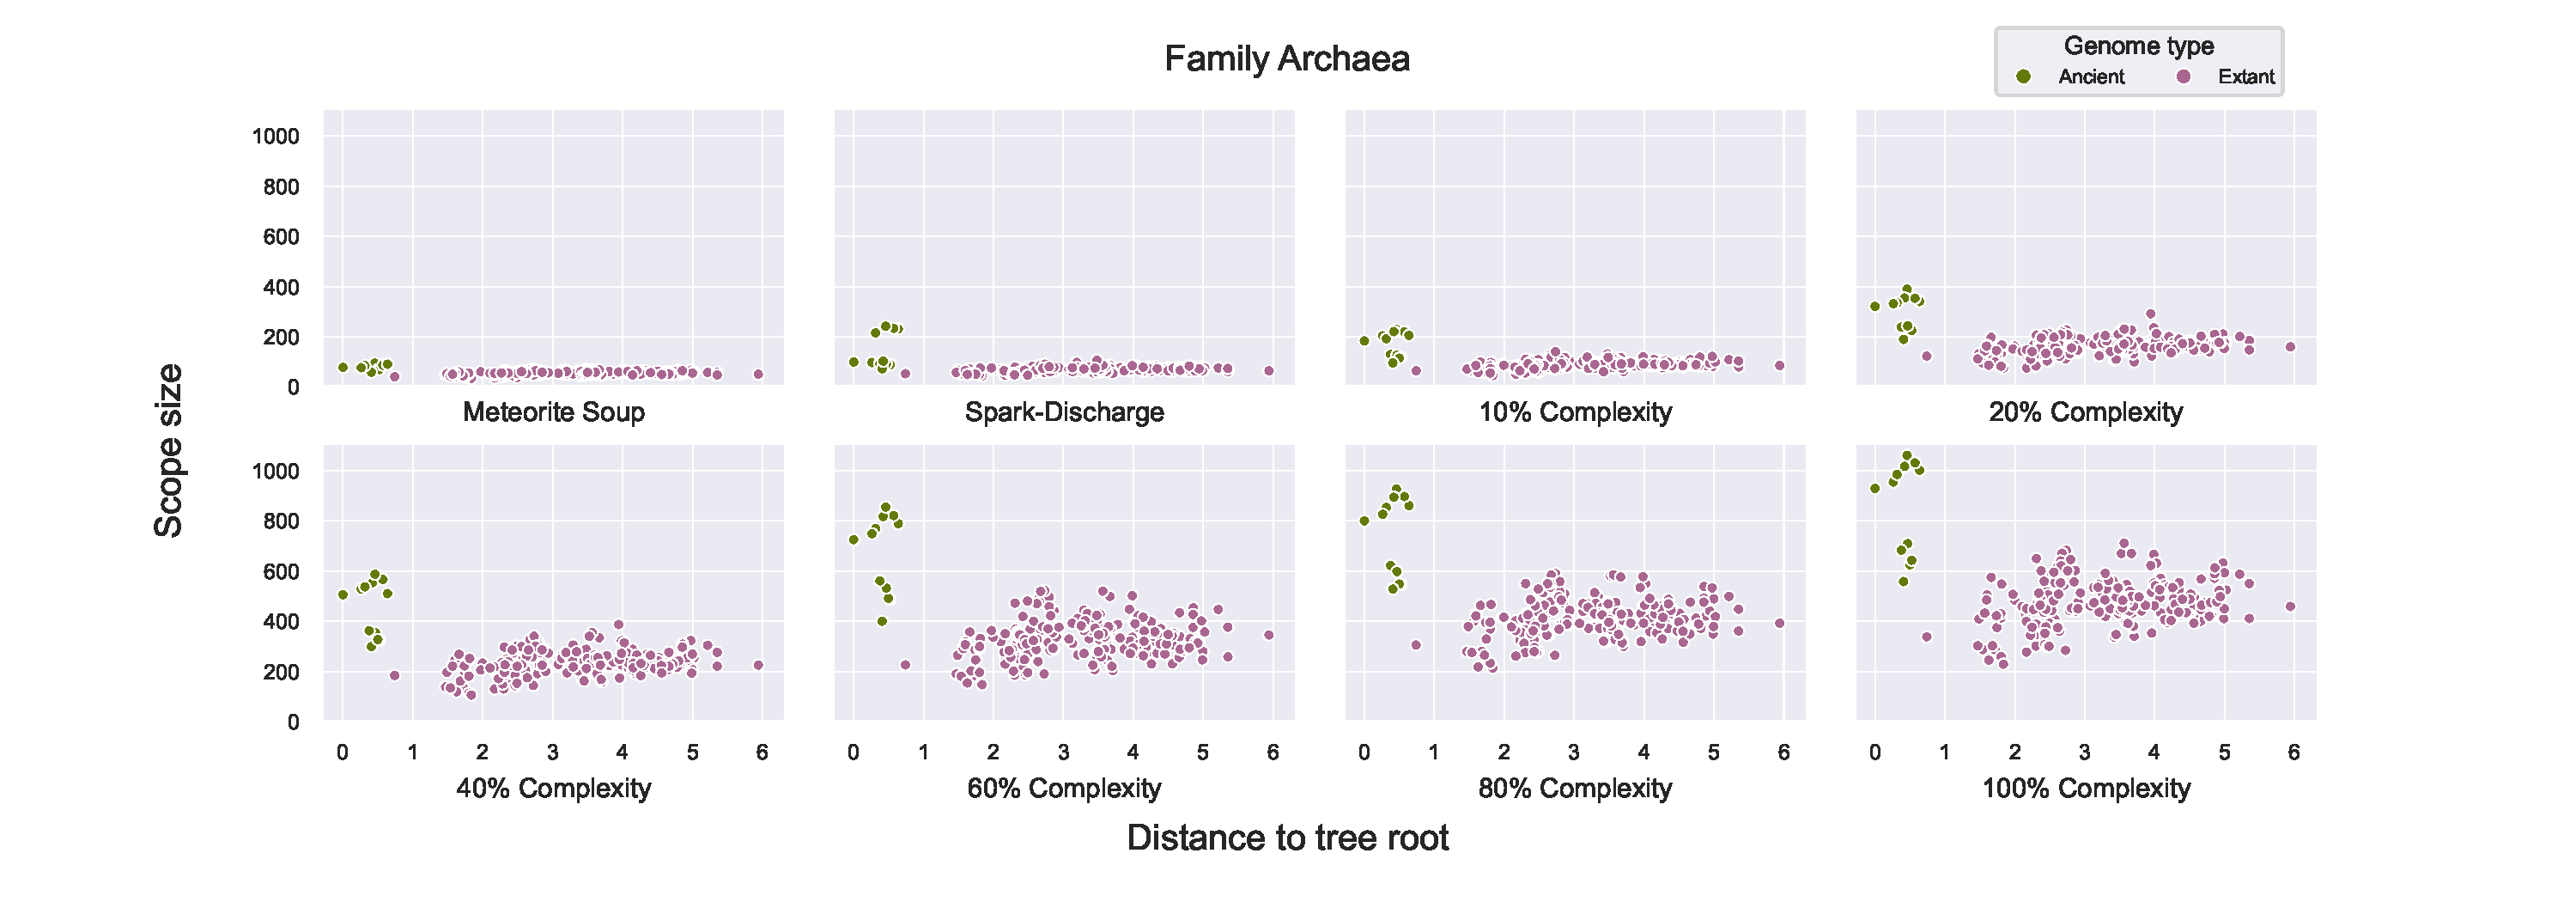
\includegraphics[width=0.95\textwidth]{scopesize_vs_disttoroot/fam4arc_ss_rootdist.pdf}
%     \caption{Family level archaea}
%     \label{famarc_scopesize}
% \end{figure}   

% \begin{figure}[H]
%     \centering
%     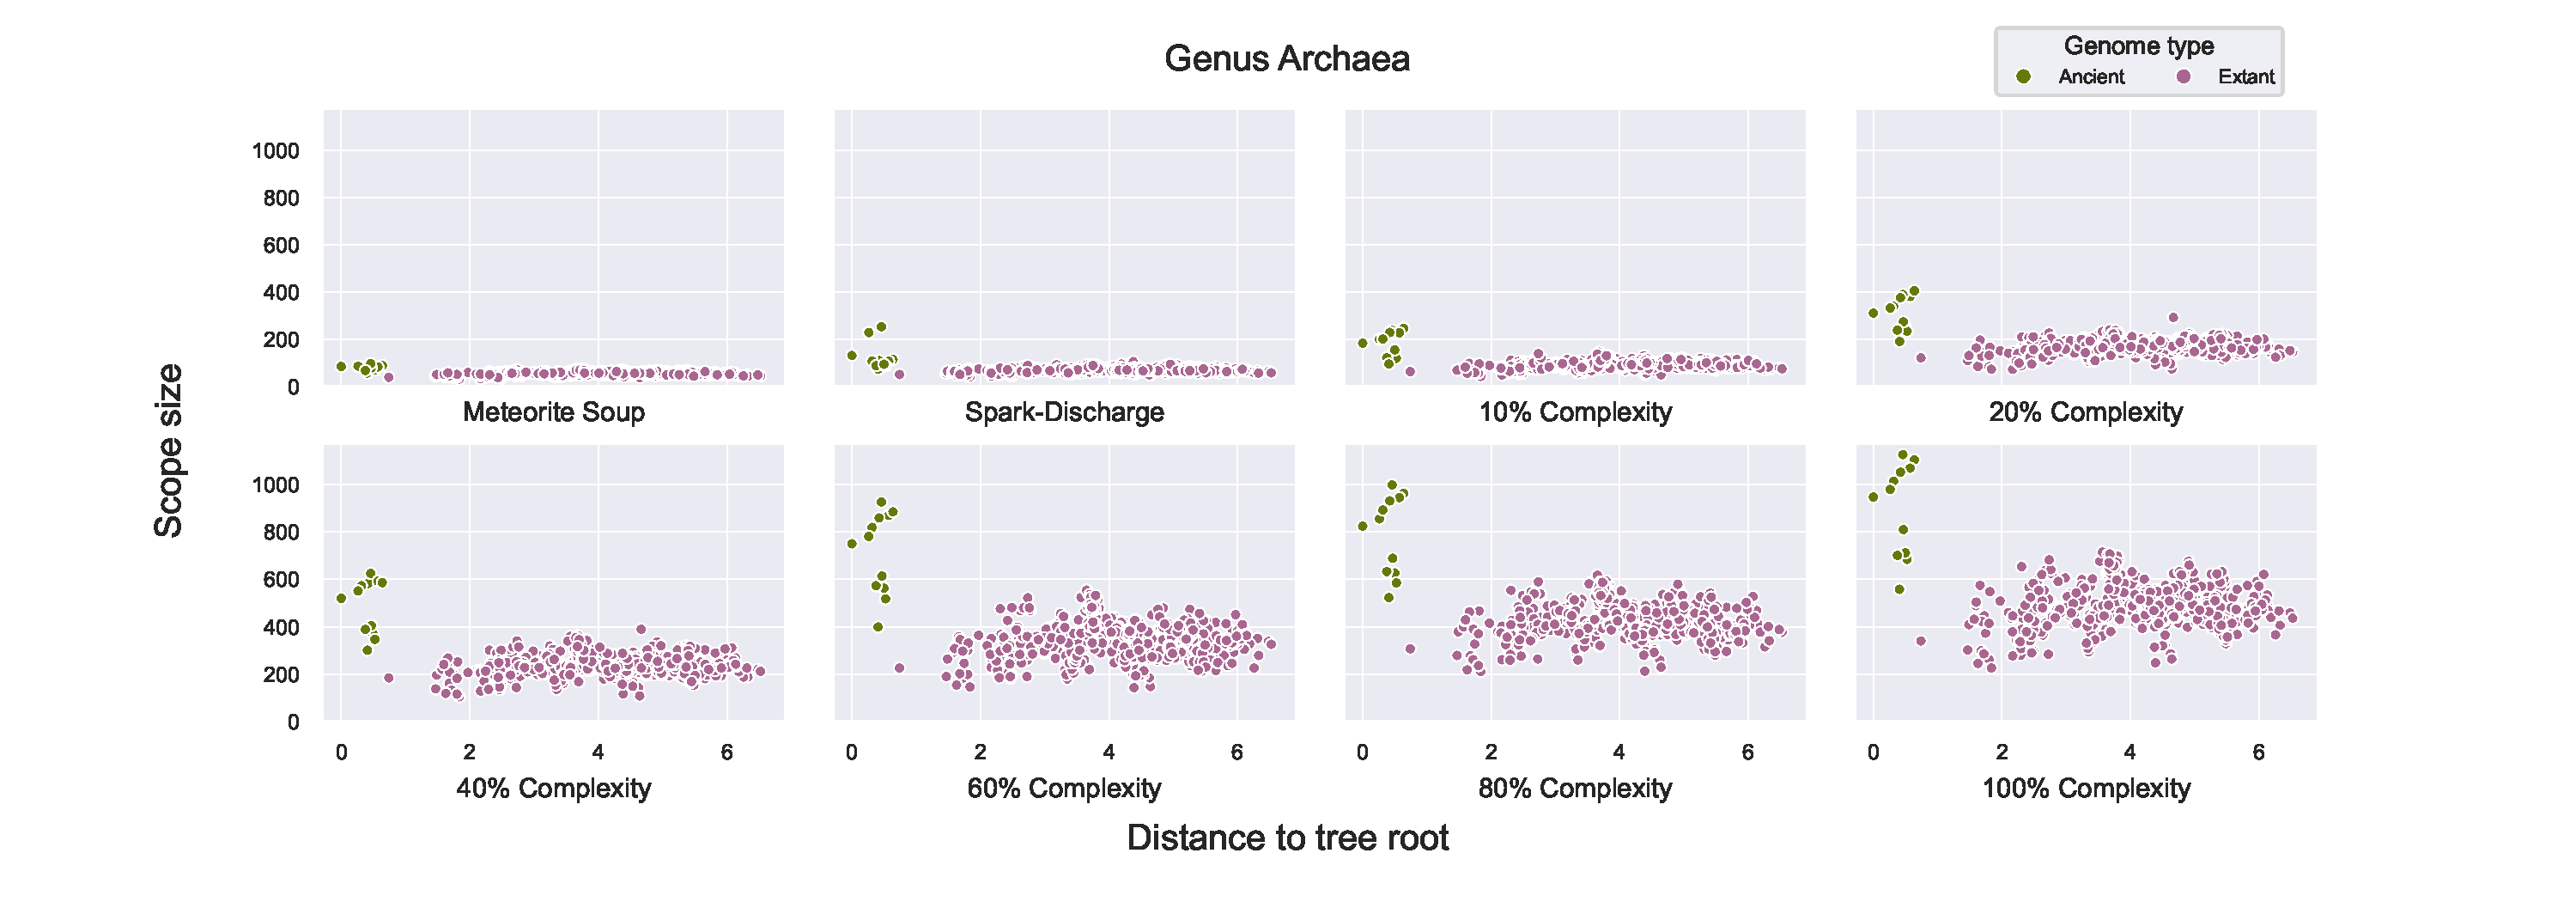
\includegraphics[width=0.95\textwidth]{scopesize_vs_disttoroot/gen4arc_ss_rootdist.pdf}
%     \caption{Genus level archaea}
%     \label{genarc_scopesize}
% \end{figure}   

% \begin{figure}[H]
%     \centering
%     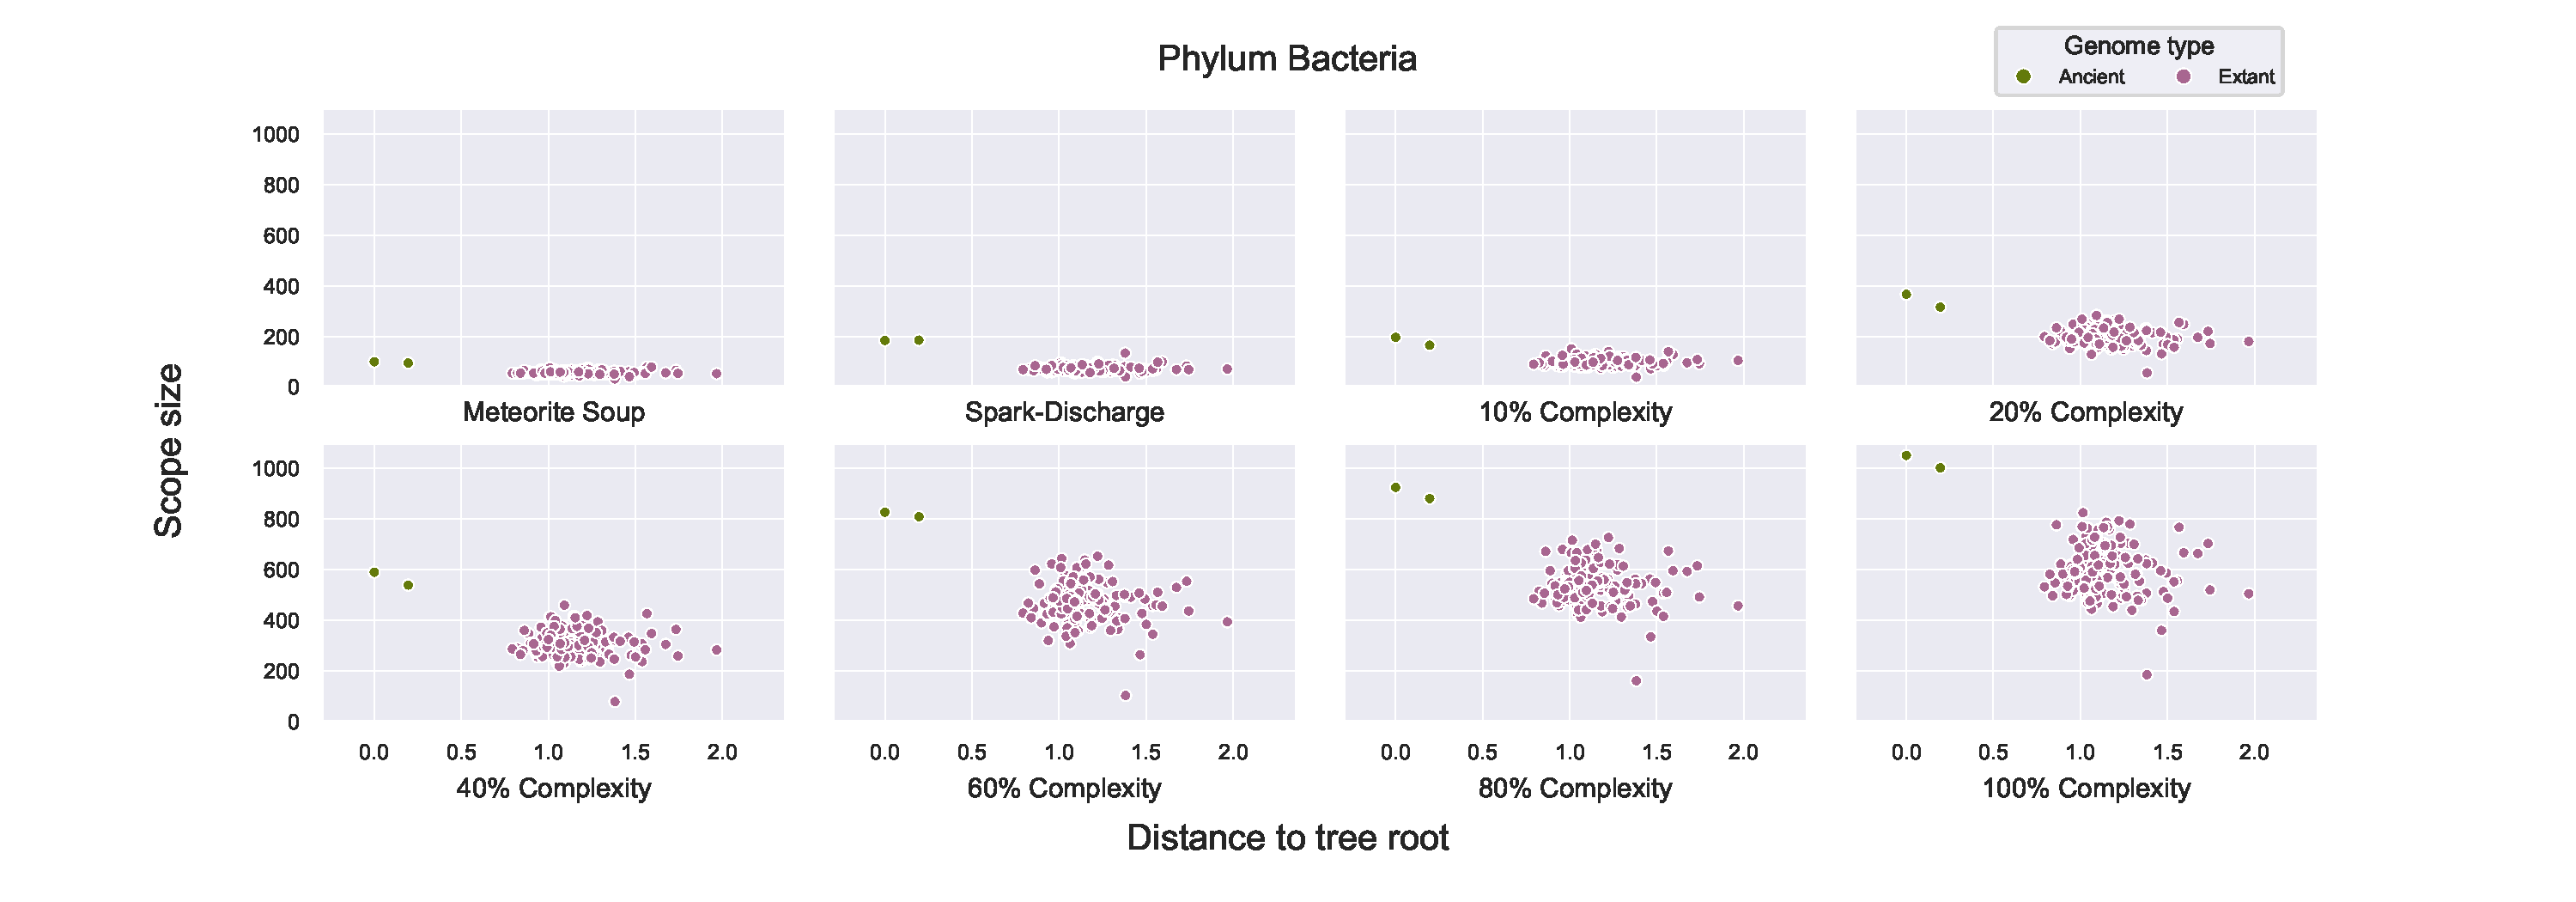
\includegraphics[width=0.95\textwidth]{scopesize_vs_disttoroot/phy4bac_ss_rootdist.pdf}
%     \caption{Phylum level bacteria}
%     \label{phybac_scopesize}
% \end{figure}   

% \begin{figure}[H]
%     \centering
%     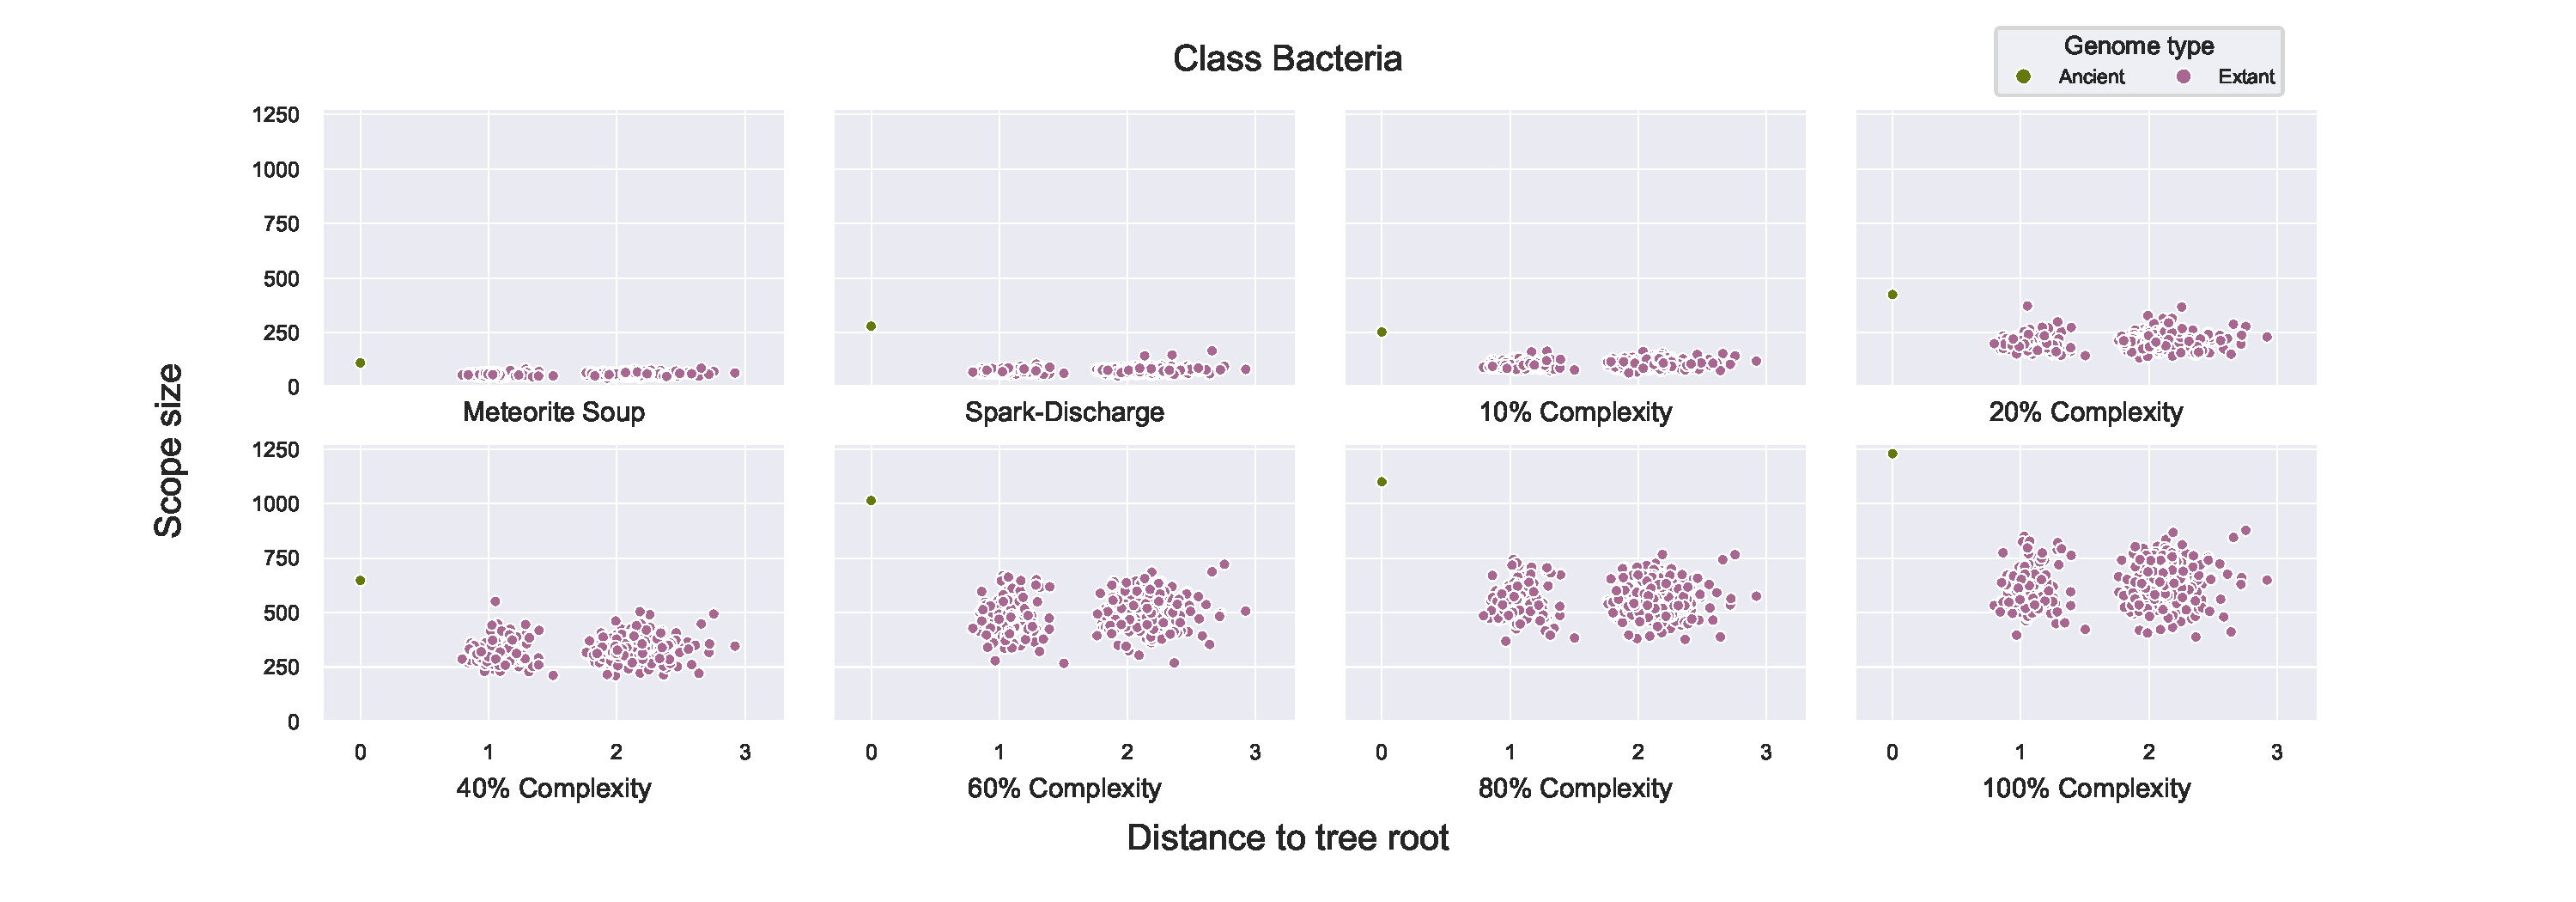
\includegraphics[width=0.95\textwidth]{scopesize_vs_disttoroot/cla4bac_ss_rootdist.pdf}
%     \caption{Class level bacteria}
%     \label{clabac_scopesize}
% \end{figure}   




% %\subsection*{A2. Metabolic Network Expansion}
% %\addcontentsline{toc}{subsection}{Metabolic Network Expansion}


